\section{Puzzle}\label{puzzle}
\subsection{} % 1
\begin{center}
    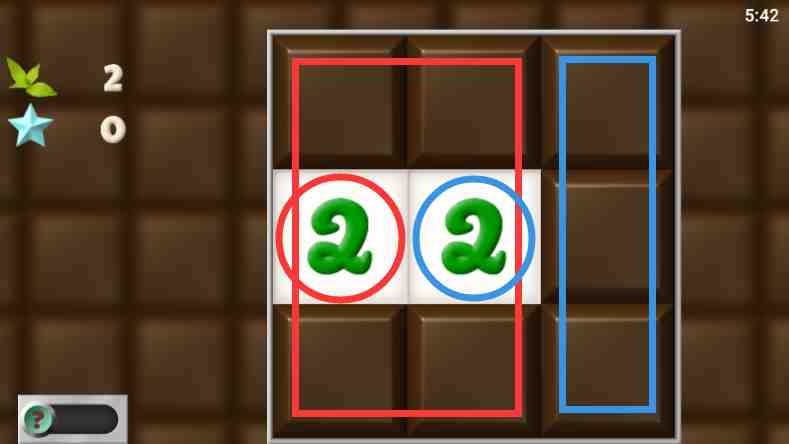
\includegraphics[width=0.7\textwidth]{puzzlelow/1-1.jpg}
\end{center}
因为红圈2,红框内有两个雷;又因为蓝圈2,蓝框内安全。
\begin{center}
    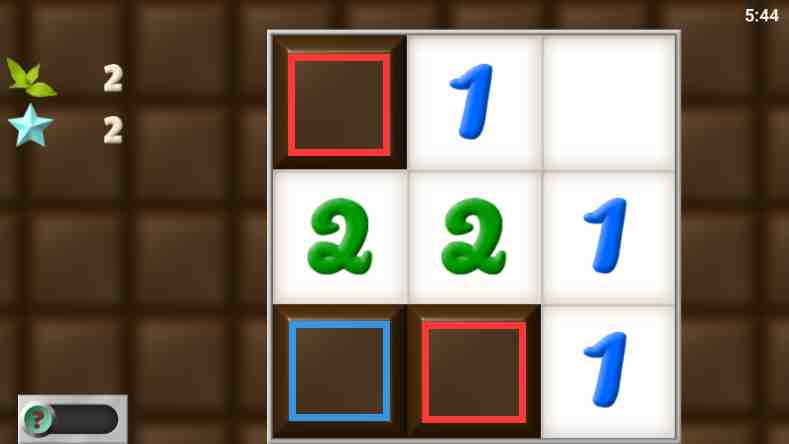
\includegraphics[width=0.7\textwidth]{puzzlelow/1-2.jpg}
\end{center}
数数,红框为雷,蓝框安全。

\subsection{} % 2
\begin{center}
    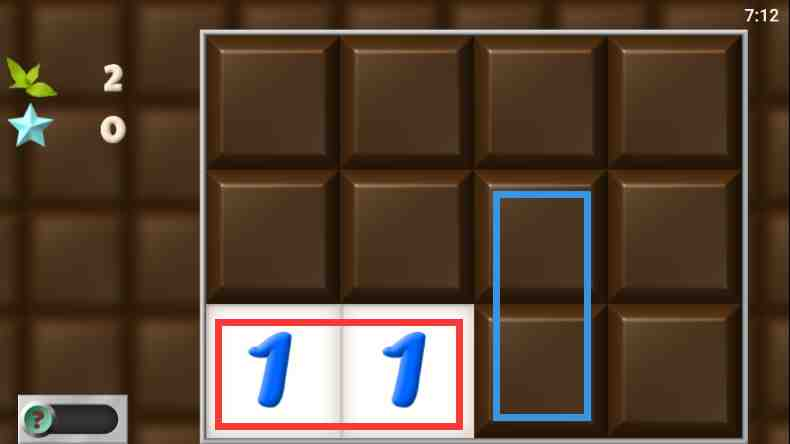
\includegraphics[width=0.7\textwidth]{puzzlelow/2-1.jpg}
\end{center}
红框11减法,蓝框安全。
\begin{center}
    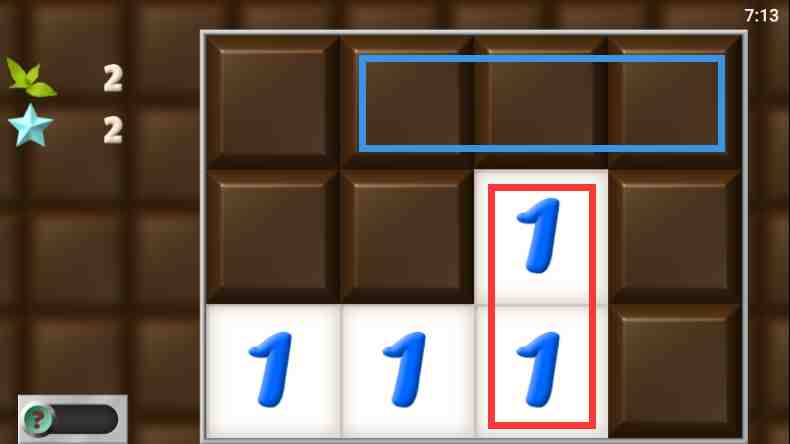
\includegraphics[width=0.7\textwidth]{puzzlelow/2-2.jpg}
\end{center}
红框11减法,蓝框安全。
\begin{center}
    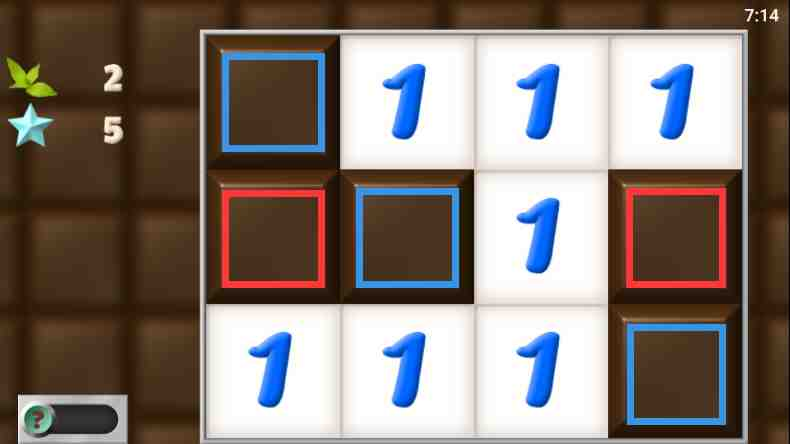
\includegraphics[width=0.7\textwidth]{puzzlelow/2-3.jpg}
\end{center}
数数,红框为雷,蓝框安全。

\subsection{} % 3
\begin{center}
    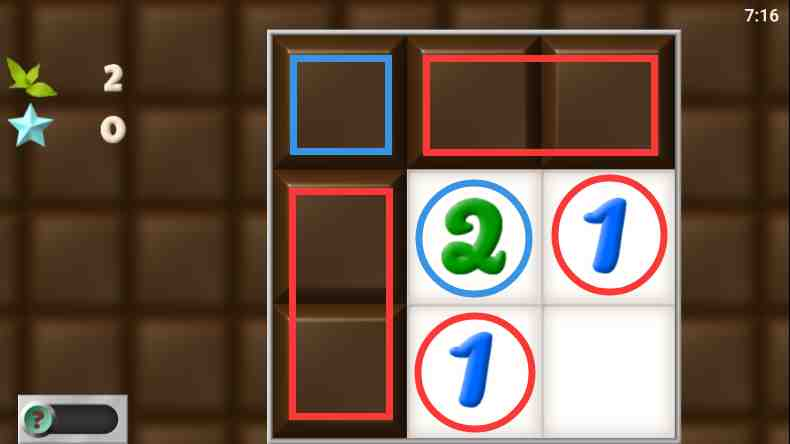
\includegraphics[width=0.7\textwidth]{puzzlelow/3-1.jpg}
\end{center}
由两个红圈1,两个红框各1雷;又因为蓝圈2,蓝框安全。
\begin{center}
    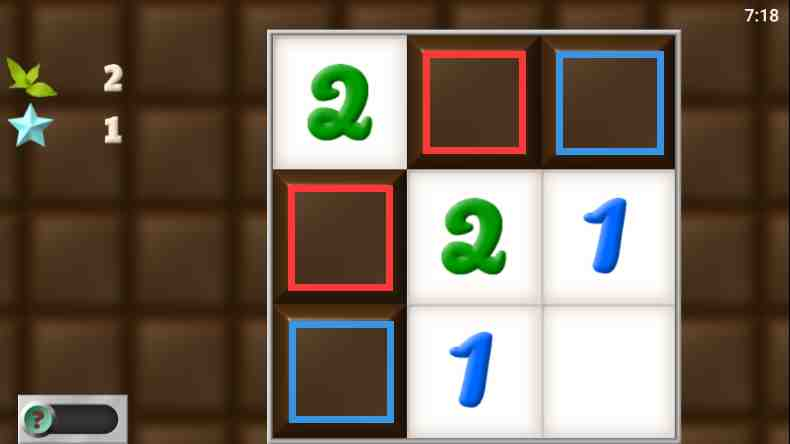
\includegraphics[width=0.7\textwidth]{puzzlelow/3-2.jpg}
\end{center}
数数,红框为雷,蓝框安全。

\subsection{} % 4
\begin{center}
    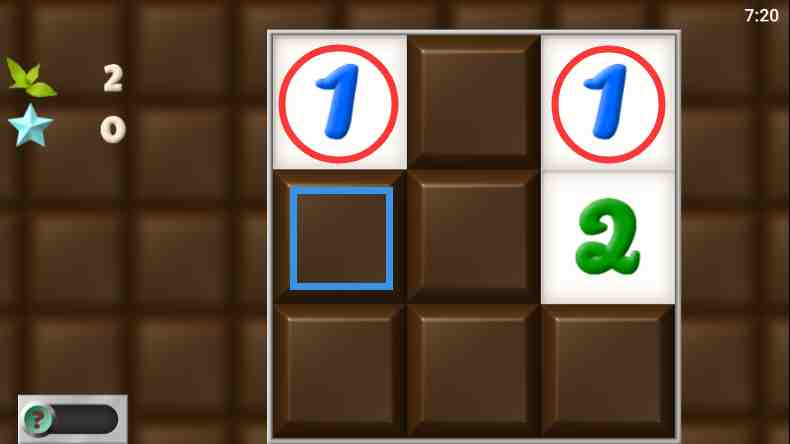
\includegraphics[width=0.7\textwidth]{puzzlelow/4-1.jpg}
\end{center}
红圈11减法,蓝框安全。
\begin{center}
    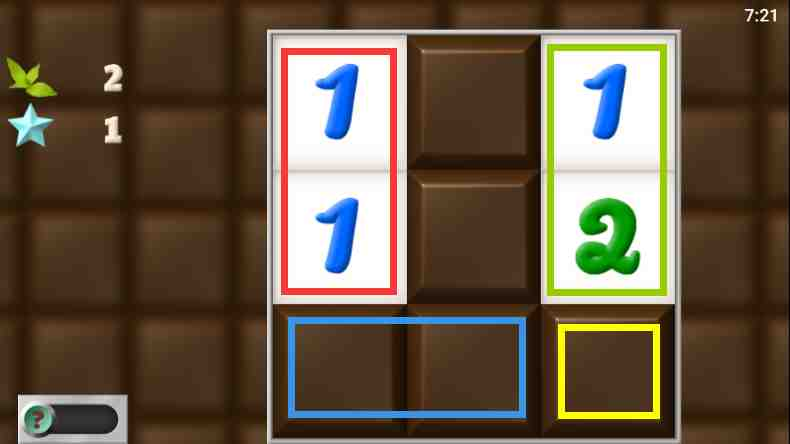
\includegraphics[width=0.7\textwidth]{puzzlelow/4-2.jpg}
\end{center}
红框11减法,蓝框安全。再用绿框12减法,黄框为雷。
\begin{center}
    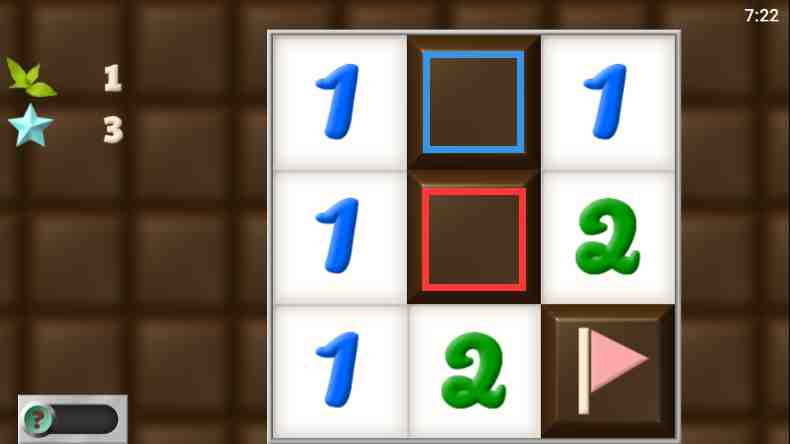
\includegraphics[width=0.7\textwidth]{puzzlelow/4-3.jpg}
\end{center}
数数,红框为雷,蓝框安全。

\subsection{} % 5
\begin{center}
    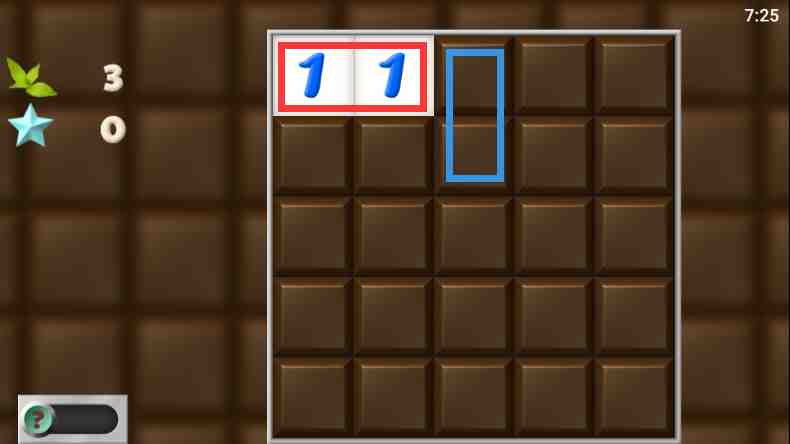
\includegraphics[width=0.7\textwidth]{puzzlelow/5-1.jpg}
\end{center}
红框11减法,蓝框安全。
\begin{center}
    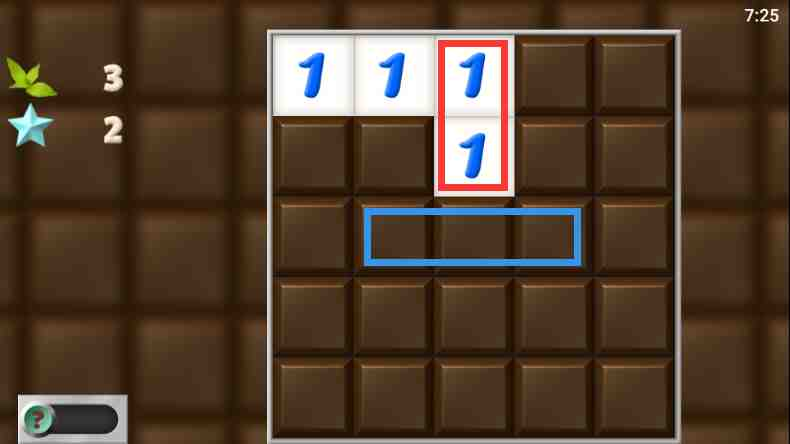
\includegraphics[width=0.7\textwidth]{puzzlelow/5-2.jpg}
\end{center}
红框11减法,蓝框安全。
\begin{center}
    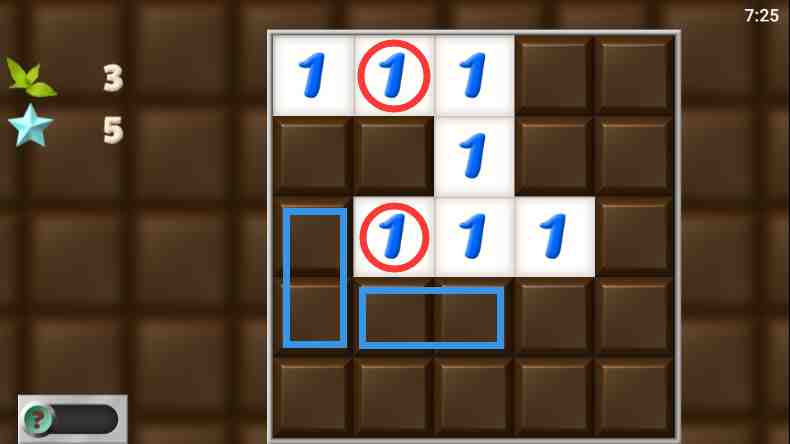
\includegraphics[width=0.7\textwidth]{puzzlelow/5-3.jpg}
\end{center}
红圈11减法,蓝框安全。
\begin{center}
    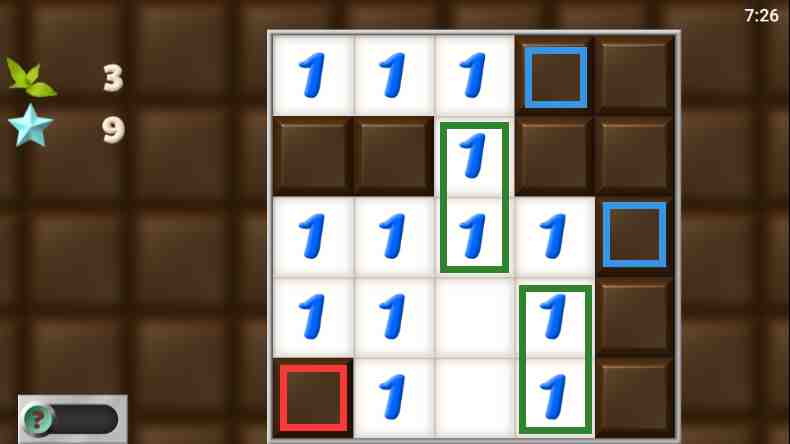
\includegraphics[width=0.7\textwidth]{puzzlelow/5-4.jpg}
\end{center}
数数,红框为雷。再分别用绿框11减法,两个蓝框安全。
\begin{center}
    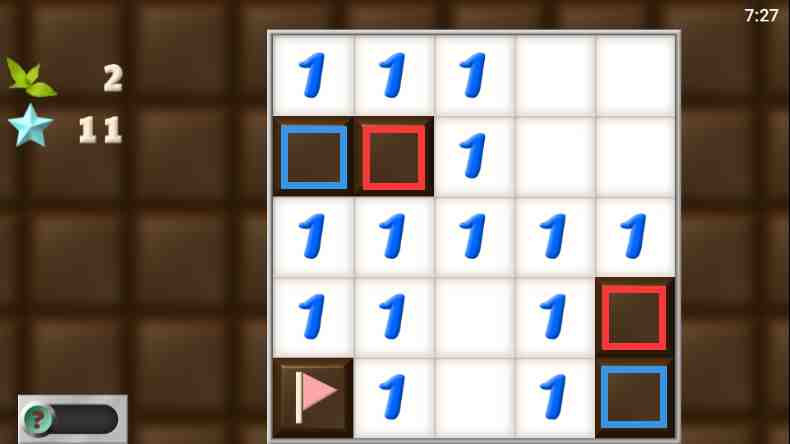
\includegraphics[width=0.7\textwidth]{puzzlelow/5-5.jpg}
\end{center}
数数,红框为雷,蓝框安全。

\subsection{} % 6
\begin{center}
    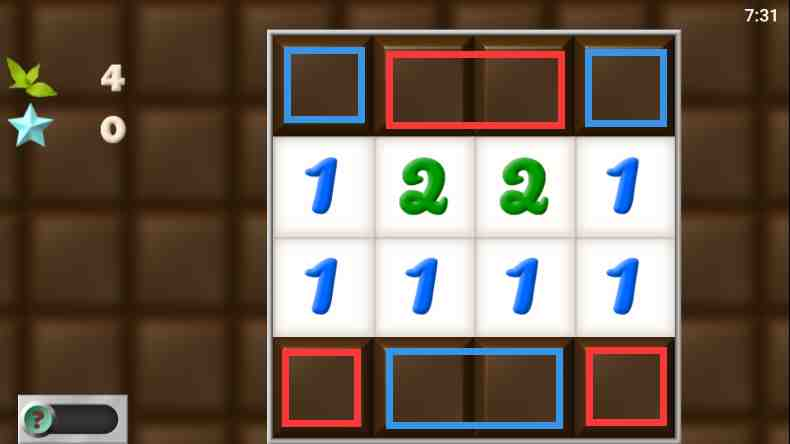
\includegraphics[width=0.7\textwidth]{puzzlelow/6-1.jpg}
\end{center}
上下分别用1221定式和1111定式,红框为雷,蓝框安全。

\subsection{} % 7
\begin{center}
    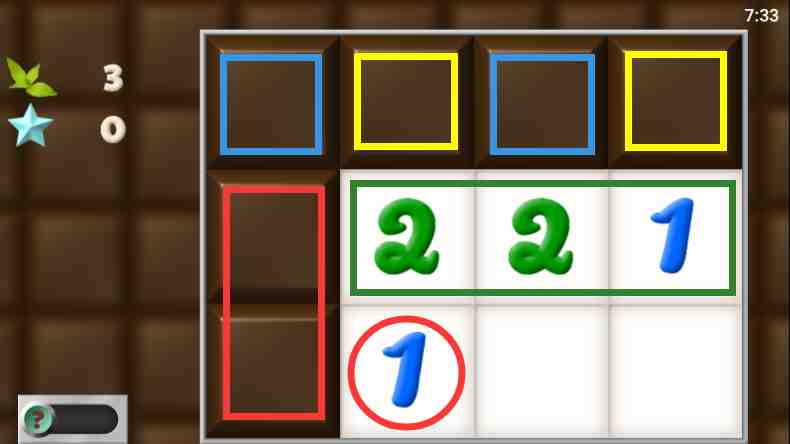
\includegraphics[width=0.7\textwidth]{puzzlelow/7-1.jpg}
\end{center}
由红圈1,红框有1雷;然后绿框形成121定式,黄框为雷,蓝框安全。

\subsection{} % 8
\begin{center}
    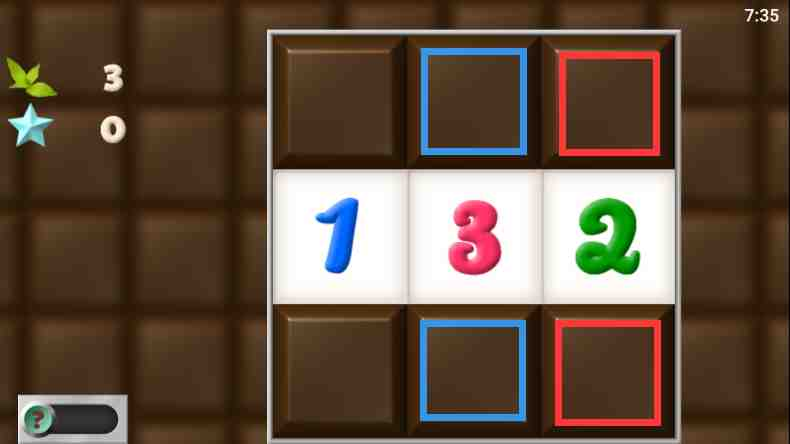
\includegraphics[width=0.7\textwidth]{puzzlelow/8-1.jpg}
\end{center}
由132定式,红框为雷,蓝框安全。

\subsection{} % 9
\begin{center}
    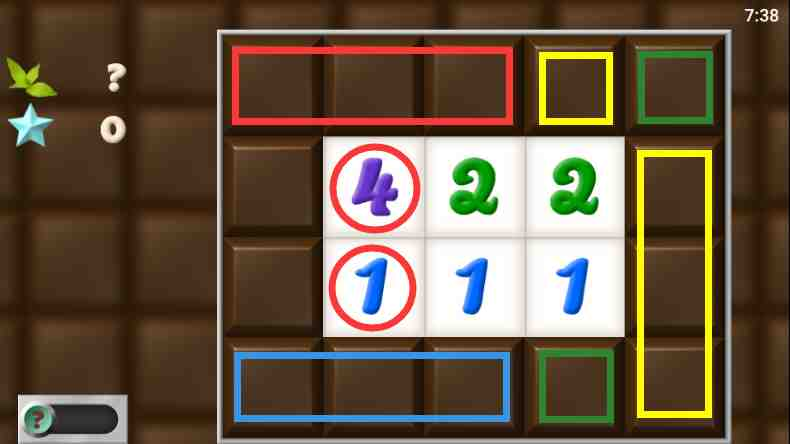
\includegraphics[width=0.7\textwidth]{puzzlelow/9-1.jpg}
\end{center}
红圈14减法,红框为雷,蓝框安全。然后数数,绿框为雷,黄框安全。
\begin{center}
    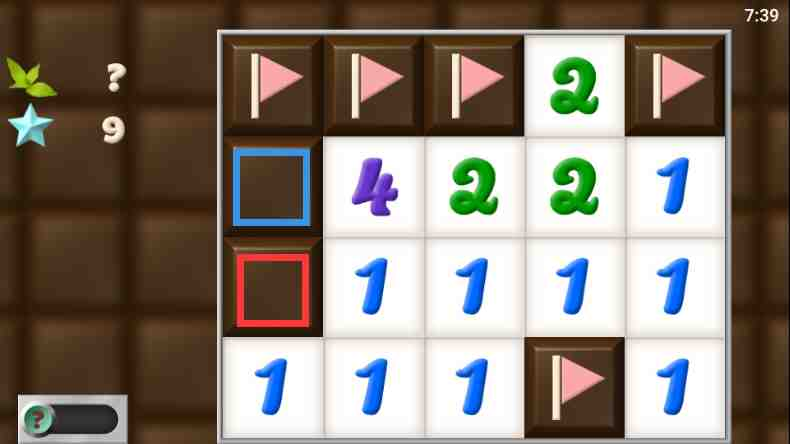
\includegraphics[width=0.7\textwidth]{puzzlelow/9-2.jpg}
\end{center}
数数,红框为雷,蓝框安全。

\subsection{} % 10
\begin{center}
    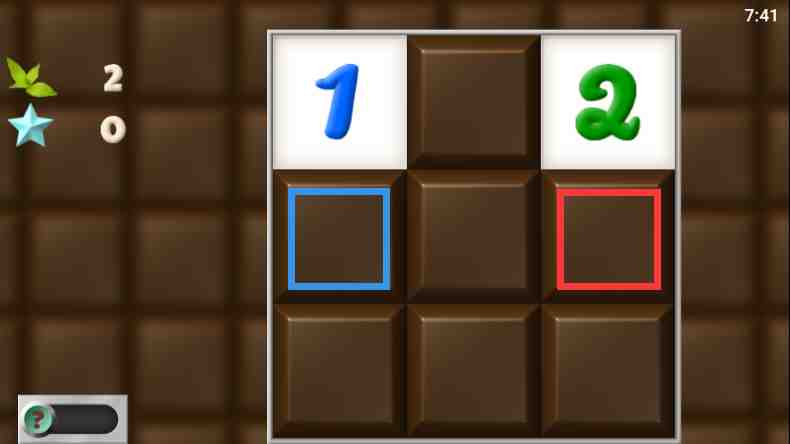
\includegraphics[width=0.7\textwidth]{puzzlelow/10-1.jpg}
\end{center}
12减法,红框为雷,蓝框安全。
\begin{center}
    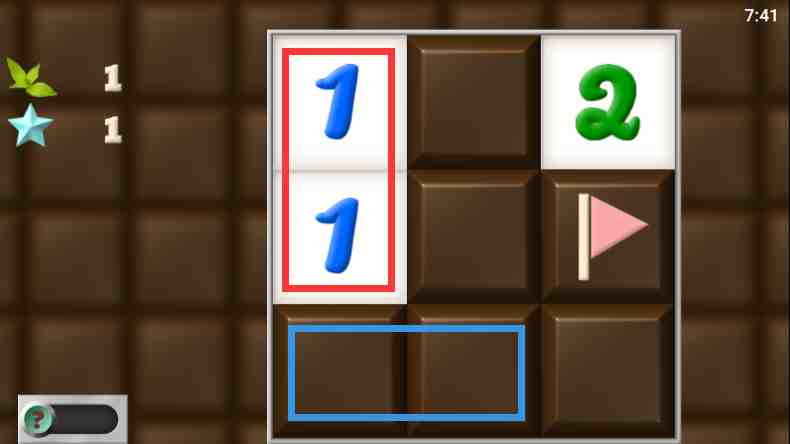
\includegraphics[width=0.7\textwidth]{puzzlelow/10-2.jpg}
\end{center}
红框11减法,蓝框安全。
\begin{center}
    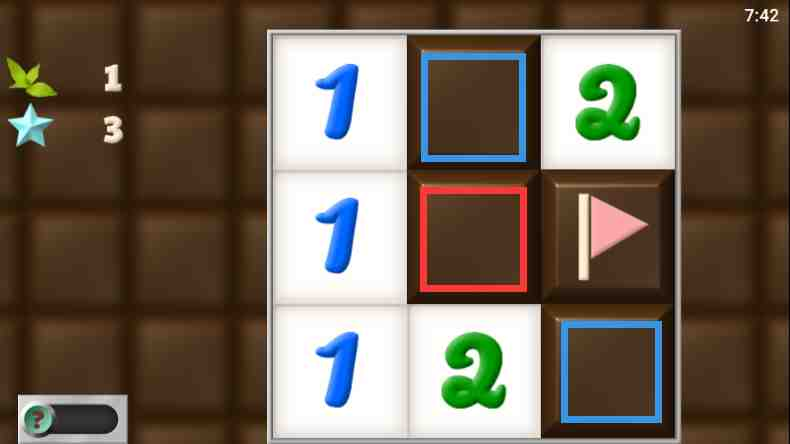
\includegraphics[width=0.7\textwidth]{puzzlelow/10-3.jpg}
\end{center}
数数,红框为雷,蓝框安全。

\subsection{} % 11
\begin{center}
    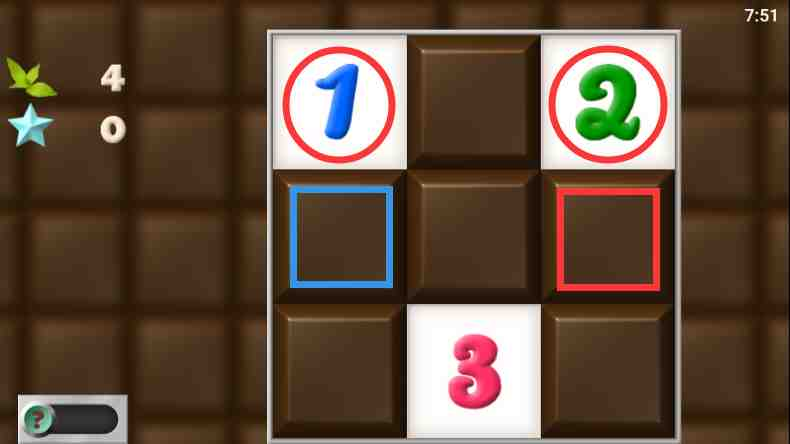
\includegraphics[width=0.7\textwidth]{puzzlelow/11-1.jpg}
\end{center}
红圈12减法,红框为雷,蓝框安全。
\begin{center}
    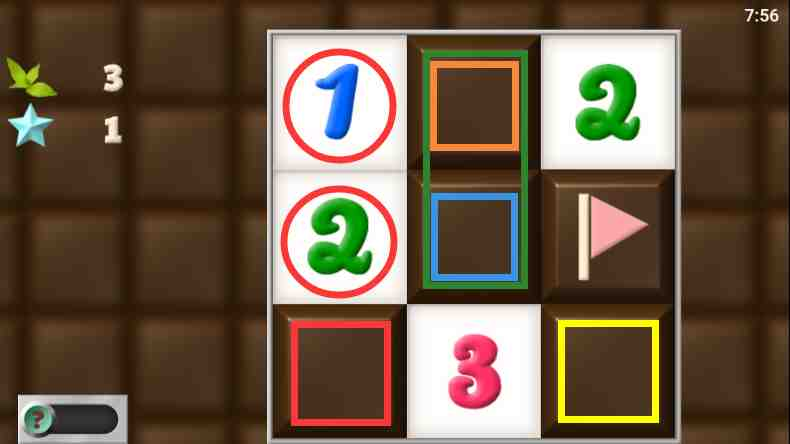
\includegraphics[width=0.7\textwidth]{puzzlelow/11-2.jpg}
\end{center}
红圈12减法,红框为雷,绿框有1雷;再数雷,排除绿框1雷,得黄框为雷。数数,橙框为雷,蓝框安全。

\subsection{} % 12
\begin{center}
    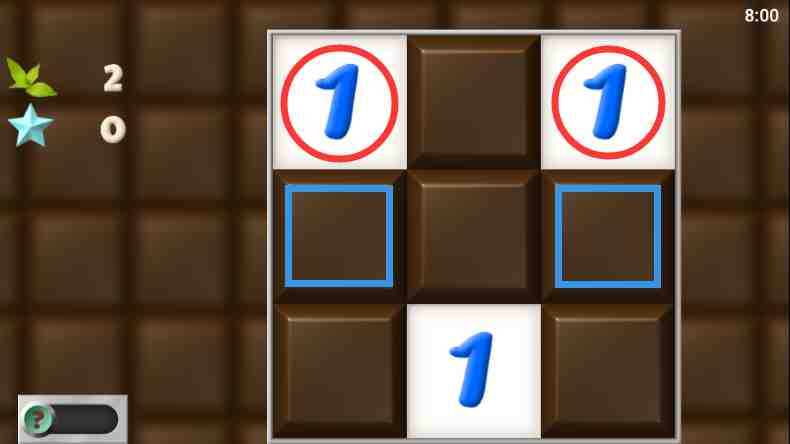
\includegraphics[width=0.7\textwidth]{puzzlelow/12-1.jpg}
\end{center}
红圈11减法得两个蓝框相等,又因为剩下一个1,两个蓝框均安全。
\begin{center}
    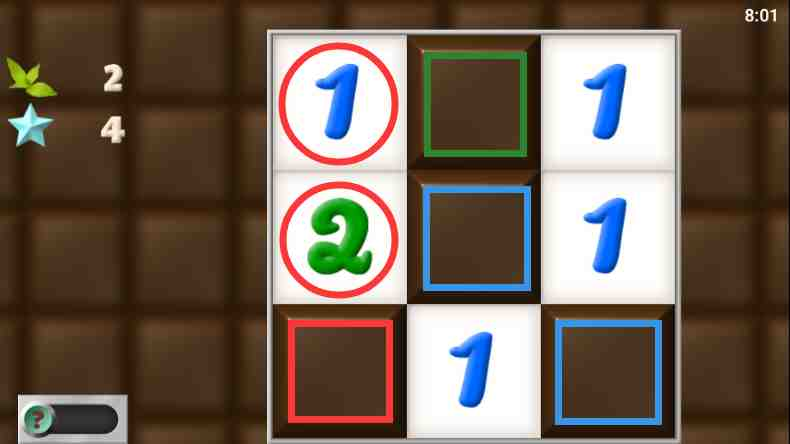
\includegraphics[width=0.7\textwidth]{puzzlelow/12-2.jpg}
\end{center}
红圈12减法,红框为雷。数数,绿框为雷,蓝框安全。

\subsection{} % 13
\begin{center}
    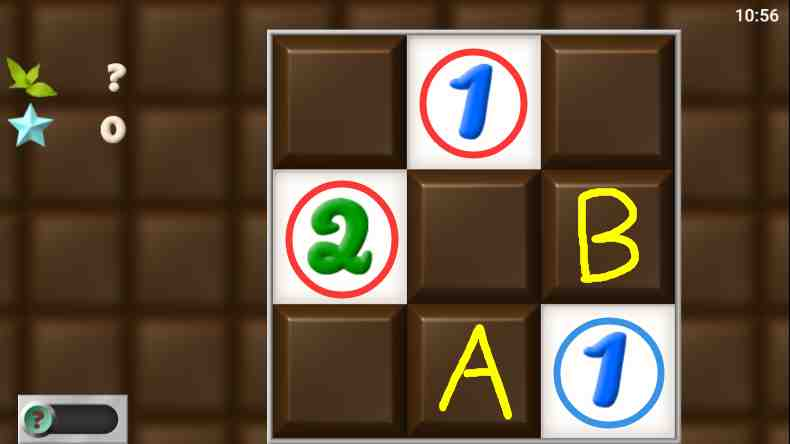
\includegraphics[width=0.7\textwidth]{puzzlelow/13-1.jpg}
\end{center}
红圈12减法得$A\ge B$,又因为蓝圈1,$B$安全。
\begin{center}
    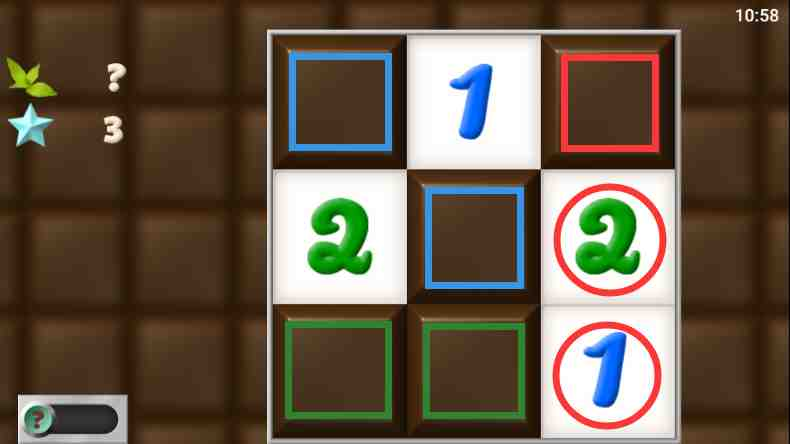
\includegraphics[width=0.7\textwidth]{puzzlelow/13-2.jpg}
\end{center}
红圈12减法,红框为雷。数数,绿框为雷,蓝框安全。

\subsection{} % 14
\begin{center}
    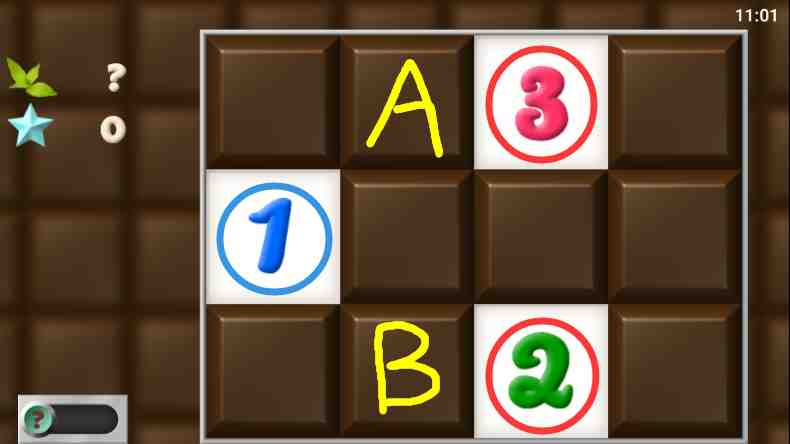
\includegraphics[width=0.7\textwidth]{puzzlelow/14-1.jpg}
\end{center}
红圈23减法得$A\ge B$,又因为蓝圈1,$B$安全。
\begin{center}
    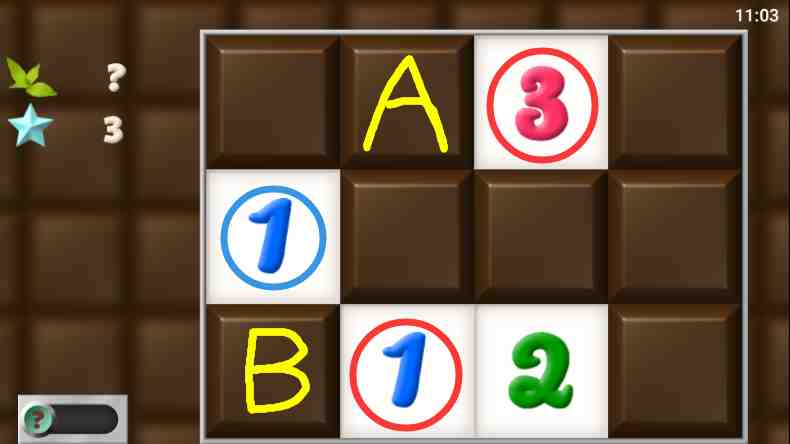
\includegraphics[width=0.7\textwidth]{puzzlelow/14-2.jpg}
\end{center}
红圈13减法得$A\ge B$,又因为蓝圈1,$B$安全。
\begin{center}
    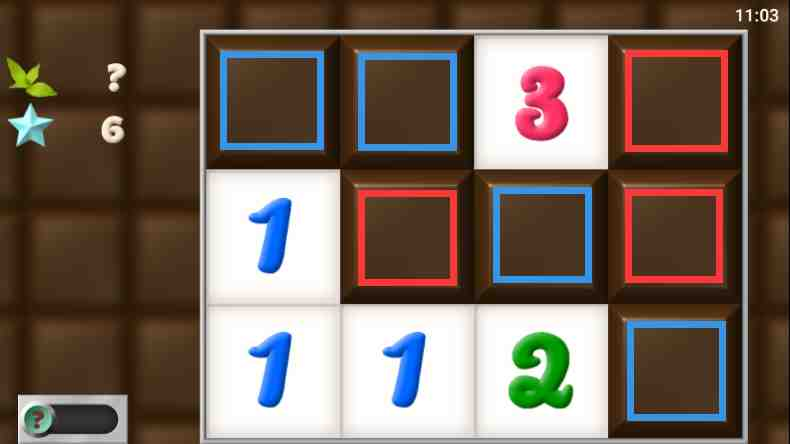
\includegraphics[width=0.7\textwidth]{puzzlelow/14-3.jpg}
\end{center}
数数,红框为雷,蓝框安全。

\subsection{} % 15
\begin{center}
    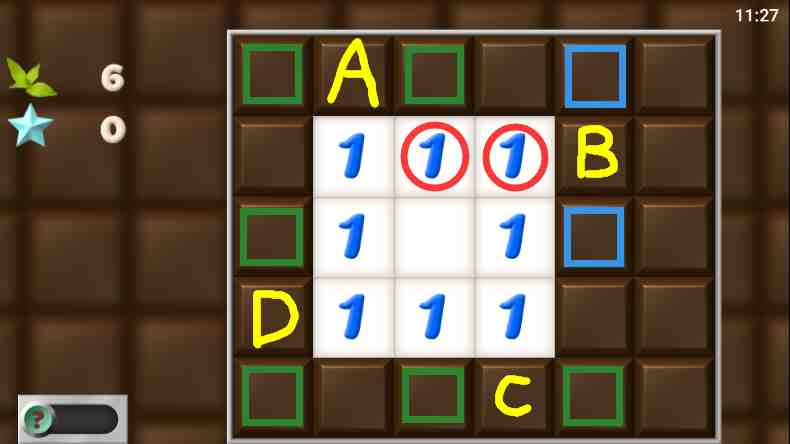
\includegraphics[width=0.7\textwidth]{puzzlelow/15-1.jpg}
\end{center}
红圈11减法得$A\ge B$,同理$B\ge C$,$C\ge D$,$D\ge A$;所以$A=B=C=D$。考虑$A=B$,再用红圈11做减法得到蓝框安全,同理绿框安全。
\begin{center}
    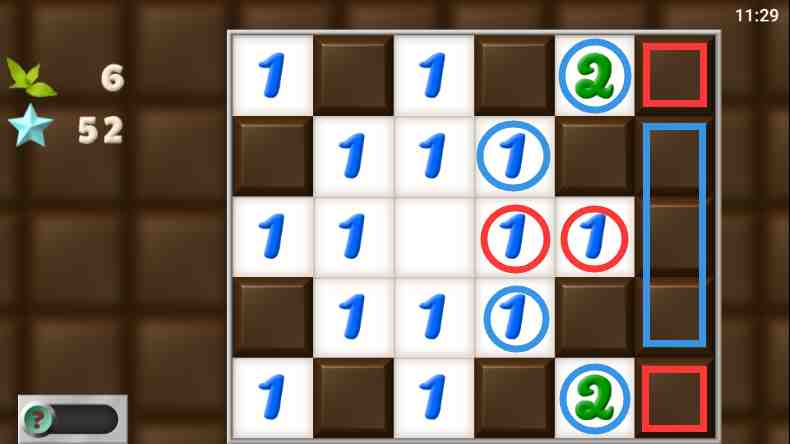
\includegraphics[width=0.7\textwidth]{puzzlelow/15-2.jpg}
\end{center}
红圈11减法得蓝框安全。再分别用两个蓝圈12减法得红框为雷。
\begin{center}
    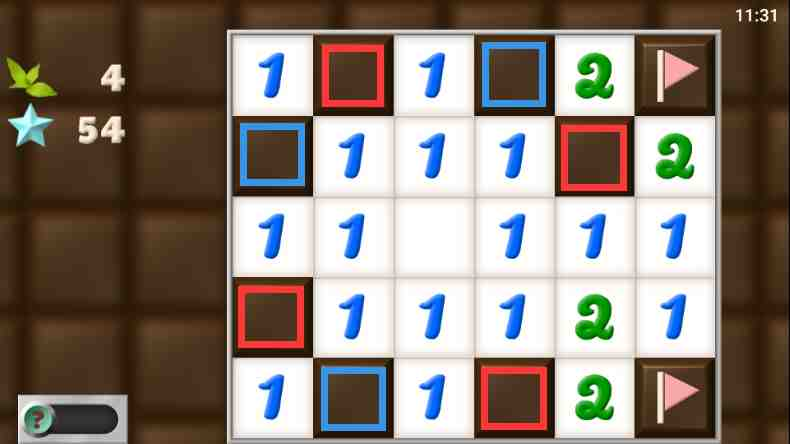
\includegraphics[width=0.7\textwidth]{puzzlelow/15-3.jpg}
\end{center}
数数,红框为雷,蓝框安全。

\subsection{} % 16
\begin{center}
    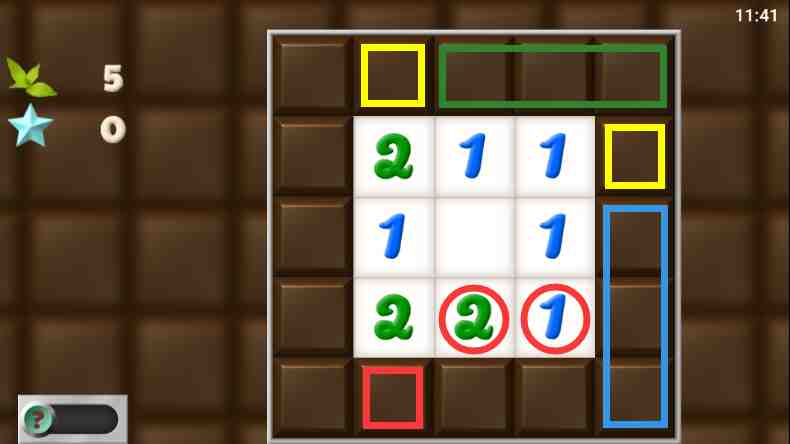
\includegraphics[width=0.7\textwidth]{puzzlelow/16-1.jpg}
\end{center}
红圈12减法得红框为雷,蓝框安全。数数,黄框为雷,绿框安全。
\begin{center}
    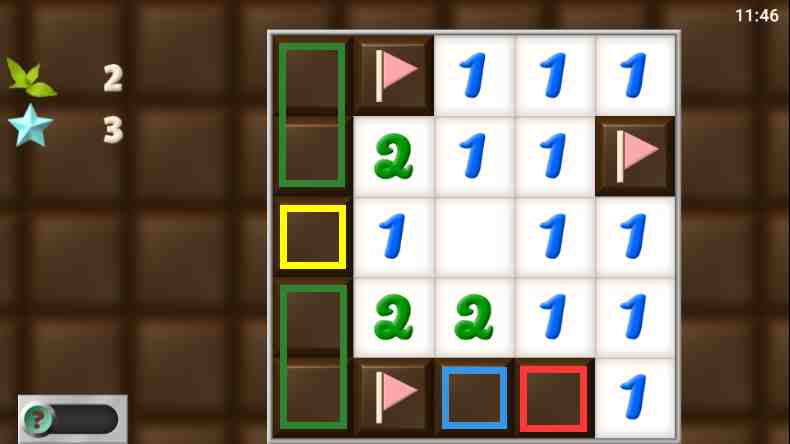
\includegraphics[width=0.7\textwidth]{puzzlelow/16-2.jpg}
\end{center}
数数,红框为雷,蓝框安全。数雷,剩下一个雷必须由左边212共用,所以黄框为雷,绿框安全。

\subsection{} % 17
\begin{center}
    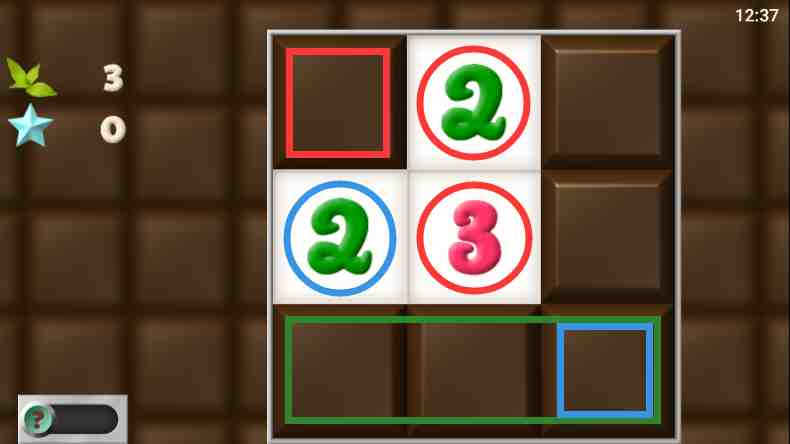
\includegraphics[width=0.7\textwidth]{puzzlelow/17-1.jpg}
\end{center}
红圈23减法得绿框有1雷;绿框再和蓝圈2做减法得红框为雷,蓝框安全。像这种用前一个减法的结论和下一个数字继续做减法的操作,我们称为连续减法。例如这里称为232连续减法。连续减法是可逆的,无论从哪边开始减,得到的结论是相同的。
\begin{center}
    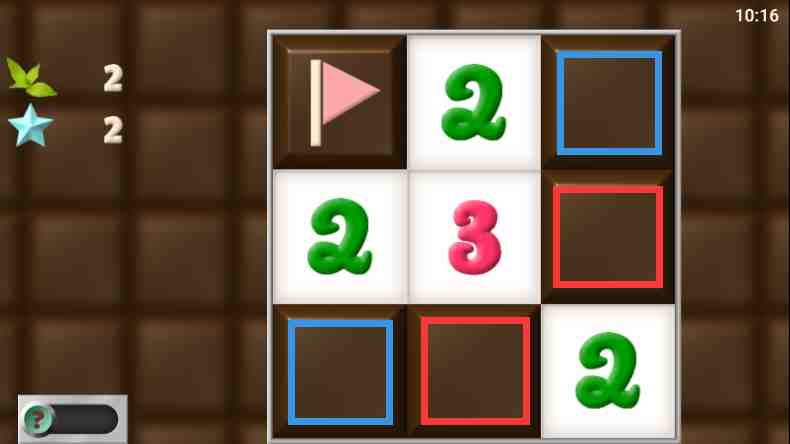
\includegraphics[width=0.7\textwidth]{puzzlelow/17-2.jpg}
\end{center}
数数,红框为雷,蓝框安全。

\subsection{} % 18
\begin{center}
    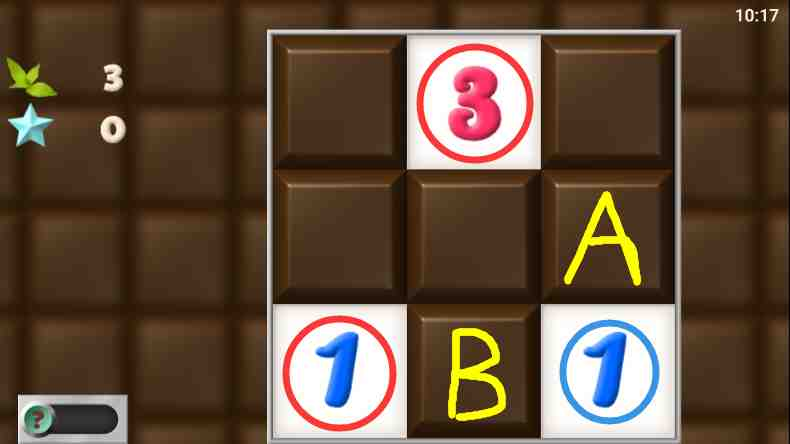
\includegraphics[width=0.7\textwidth]{puzzlelow/18-1.jpg}
\end{center}
红圈13减法得$A\ge B$,又因为蓝圈1,$B$安全。
\begin{center}
    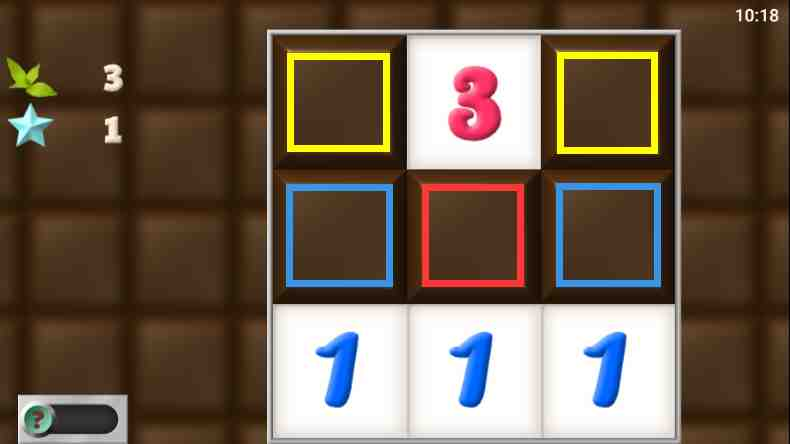
\includegraphics[width=0.7\textwidth]{puzzlelow/18-2.jpg}
\end{center}
111定式,红框为雷,蓝框安全。数数,黄框为雷。

\subsection{} % 19
\begin{center}
    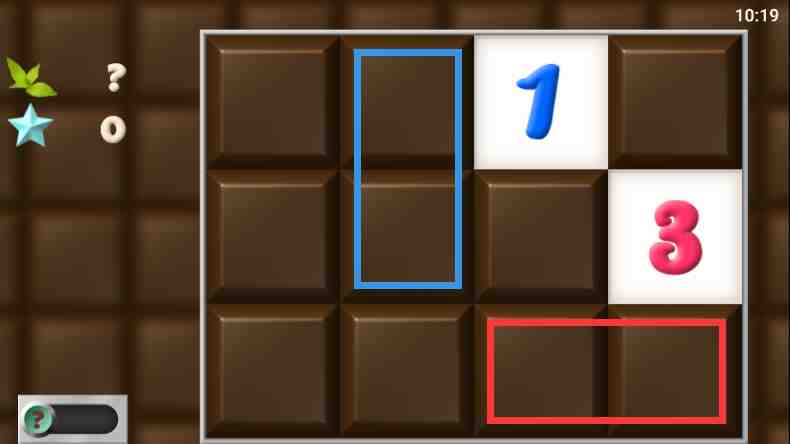
\includegraphics[width=0.7\textwidth]{puzzlelow/19-1.jpg}
\end{center}
红圈13减法得红框为雷,蓝框安全。
\begin{center}
    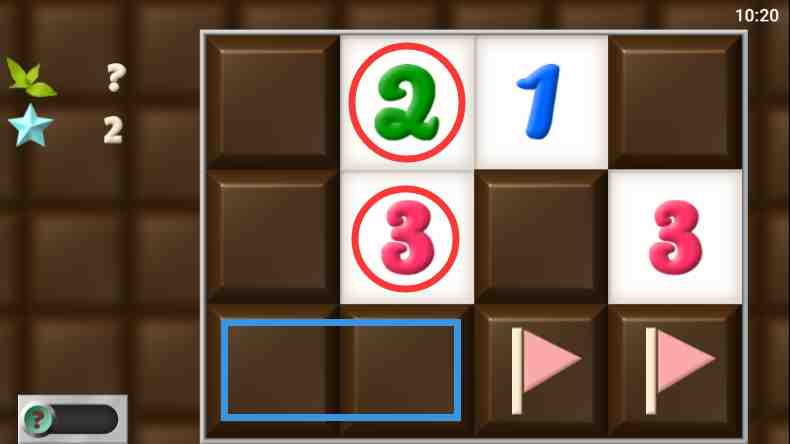
\includegraphics[width=0.7\textwidth]{puzzlelow/19-2.jpg}
\end{center}
红圈23减法得蓝框安全。
\begin{center}
    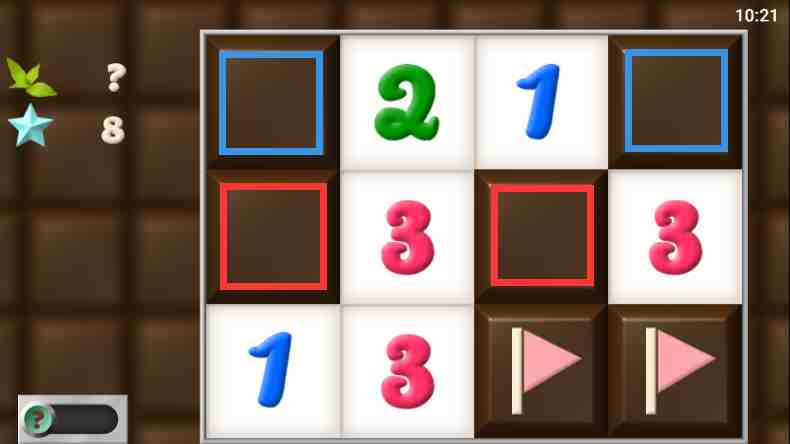
\includegraphics[width=0.7\textwidth]{puzzlelow/19-3.jpg}
\end{center}
数数,红框为雷,蓝框安全。

\subsection{} % 20
\begin{center}
    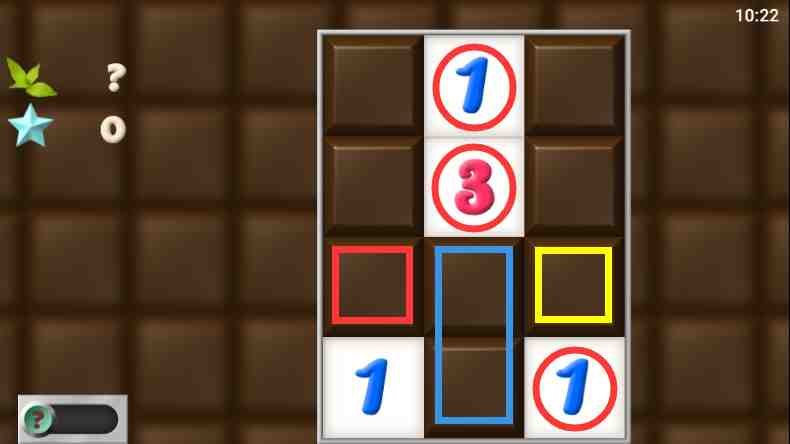
\includegraphics[width=0.7\textwidth]{puzzlelow/20-1.jpg}
\end{center}
红圈131连续减法得红框为雷,同理黄框为雷。数数,蓝框安全。

\subsection{} % 21
\begin{center}
    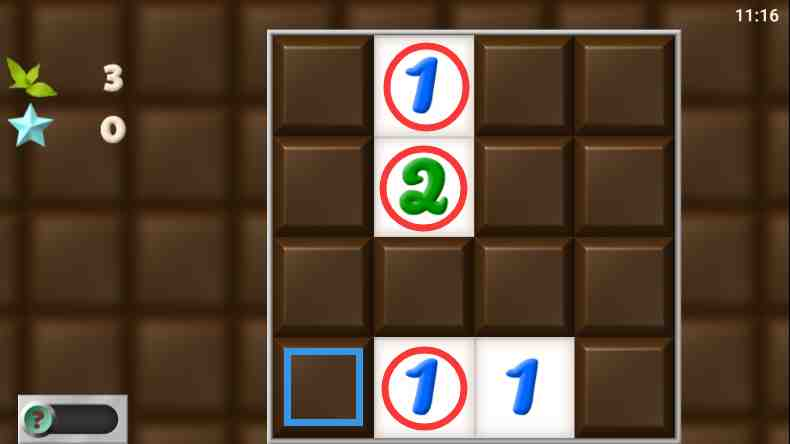
\includegraphics[width=0.7\textwidth]{puzzlelow/21-1.jpg}
\end{center}
红圈121连续减法得蓝框安全。
\begin{center}
    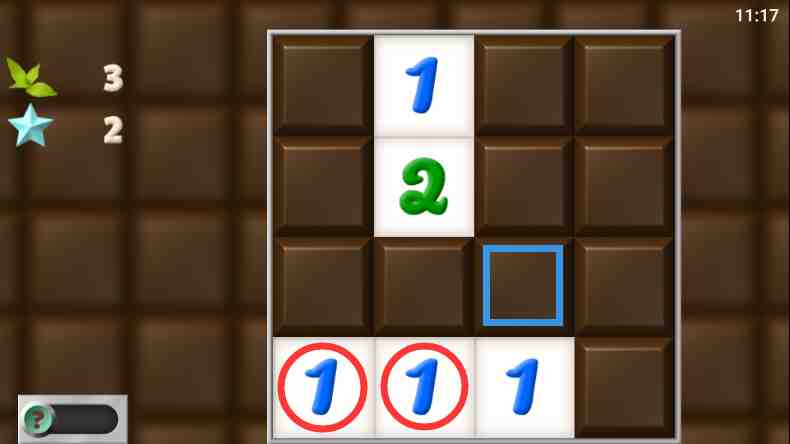
\includegraphics[width=0.7\textwidth]{puzzlelow/21-2.jpg}
\end{center}
红圈11减法得蓝框安全。
\begin{center}
    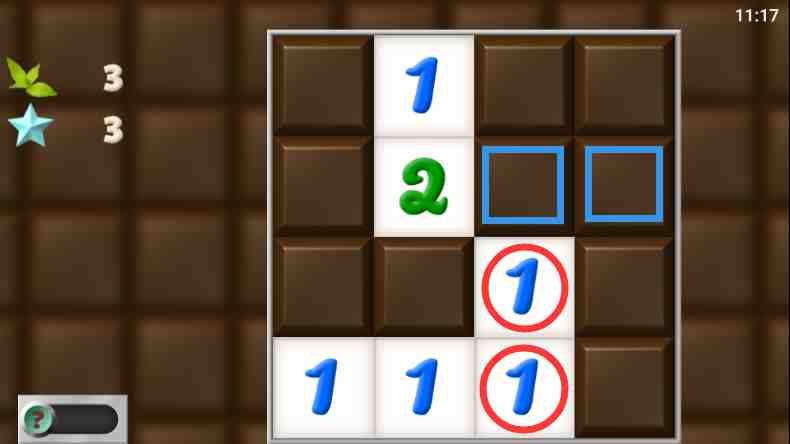
\includegraphics[width=0.7\textwidth]{puzzlelow/21-3.jpg}
\end{center}
红圈11减法得蓝框安全。
\begin{center}
    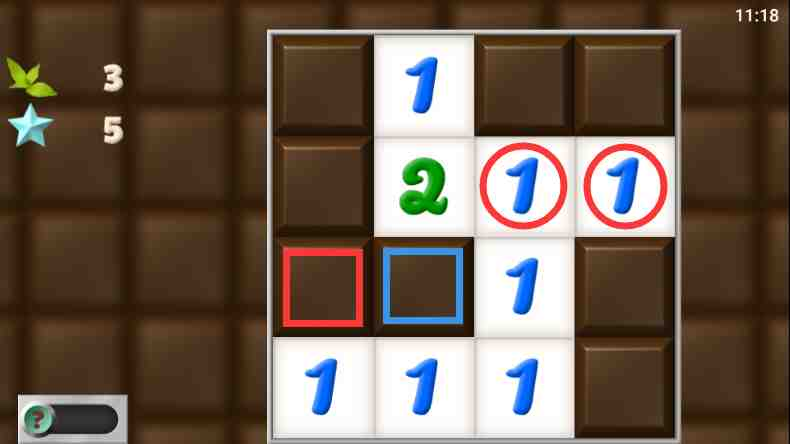
\includegraphics[width=0.7\textwidth]{puzzlelow/21-4.jpg}
\end{center}
红圈11减法得蓝框安全。数数,红框为雷。
\begin{center}
    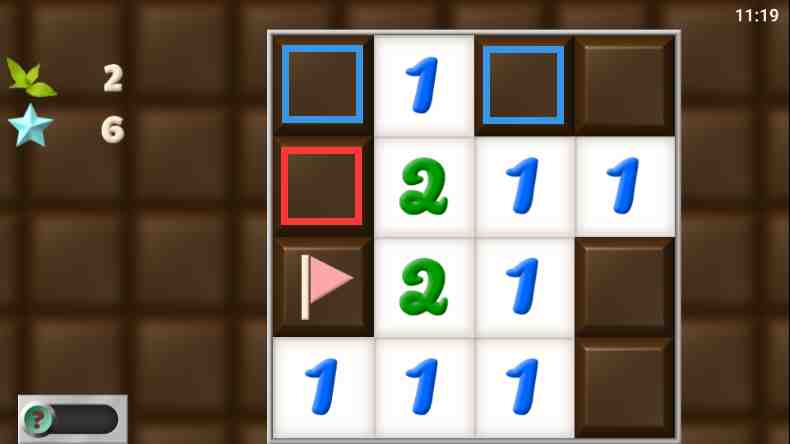
\includegraphics[width=0.7\textwidth]{puzzlelow/21-5.jpg}
\end{center}
数数,红框为雷,蓝框安全。
\begin{center}
    \includegraphics[width=0.7\textwidth]{puzzlelow/21-6.jpg}
\end{center}
数数,红框为雷,蓝框安全。

\subsection{} % 22
\begin{center}
    \includegraphics[width=0.7\textwidth]{puzzlelow/22-1.jpg}
\end{center}
红圈22减法得蓝框安全。
\begin{center}
    \includegraphics[width=0.7\textwidth]{puzzlelow/22-2.jpg}
\end{center}
红圈2321连续减法得红框为雷,蓝框安全。
\begin{center}
    \includegraphics[width=0.7\textwidth]{puzzlelow/22-3.jpg}
\end{center}
数数,红框为雷。数雷,两个绿框各有1雷,蓝框安全。
\begin{center}
    \includegraphics[width=0.7\textwidth]{puzzlelow/22-4.jpg}
\end{center}
数数,红框为雷,蓝框安全。

\subsection{} % 23
\begin{center}
    \includegraphics[width=0.7\textwidth]{puzzlelow/23-1.jpg}
\end{center}
红圈13减法得红框为雷。再用蓝圈1231连续减法得蓝框安全。
\begin{center}
    \includegraphics[width=0.7\textwidth]{puzzlelow/23-2.jpg}
\end{center}
数数,红框为雷,蓝框安全。
\begin{center}
    \includegraphics[width=0.7\textwidth]{puzzlelow/23-3.jpg}
\end{center}
数数,红框为雷,蓝框安全。

\subsection{} % 24
\begin{center}
    \includegraphics[width=0.7\textwidth]{puzzlelow/24-1.jpg}
\end{center}
两绿框各有1雷,再用红圈32减法得红框为雷,蓝框安全。
\begin{center}
    \includegraphics[width=0.7\textwidth]{puzzlelow/24-2.jpg}
\end{center}
数数,红框为雷,蓝框安全。

\subsection{} % 25
\begin{center}
    \includegraphics[width=0.7\textwidth]{puzzlelow/25-1.jpg}
\end{center}
红圈1221连续减法得蓝框安全。
\begin{center}
    \includegraphics[width=0.7\textwidth]{puzzlelow/25-2.jpg}
\end{center}
红圈121连续减法得$A=B$,又因为蓝圈1,$AB$均安全。数数,红框为雷,蓝框安全。

\subsection{} % 26
\begin{center}
    \includegraphics[width=0.7\textwidth]{puzzlelow/26-1.jpg}
\end{center}
红圈为角131定式,红框为雷,蓝框安全。数数,黄框为雷。
\begin{center}
    \includegraphics[width=0.7\textwidth]{puzzlelow/26-2.jpg}
\end{center}
数数,红框为雷,蓝框安全。

\subsection{} % 27
\begin{center}
    \includegraphics[width=0.7\textwidth]{puzzlelow/27-1.jpg}
\end{center}
红圈12减法得红框为雷,蓝框安全。
\begin{center}
    \includegraphics[width=0.7\textwidth]{puzzlelow/27-2.jpg}
\end{center}
红圈为角131定式,红框为雷。数数,蓝框安全。
\begin{center}
    \includegraphics[width=0.7\textwidth]{puzzlelow/27-3.jpg}
\end{center}
数数,红框为雷,蓝框安全。数雷,黄框为雷,绿框安全。

\subsection{} % 28
\begin{center}
    \includegraphics[width=0.7\textwidth]{puzzlelow/28-1.jpg}
\end{center}
红圈343连续减法得红框为雷。再用蓝圈232连续减法得蓝框安全。
\begin{center}
    \includegraphics[width=0.7\textwidth]{puzzlelow/28-2.jpg}
\end{center}
数数,红框为雷,蓝框安全。

\subsection{} % 29
\begin{center}
    \includegraphics[width=0.7\textwidth]{puzzlelow/29-1.jpg}
\end{center}
红圈11减法得蓝框安全。
\begin{center}
    \includegraphics[width=0.7\textwidth]{puzzlelow/29-2.jpg}
\end{center}
红圈2321连续减法得红框为雷,蓝框安全。
\begin{center}
    \includegraphics[width=0.7\textwidth]{puzzlelow/29-3.jpg}
\end{center}
红圈51减法得红框为雷。数数,蓝框安全。
\begin{center}
    \includegraphics[width=0.7\textwidth]{puzzlelow/29-4.jpg}
\end{center}
数数,红框为雷。数雷,黄框为雷,蓝框安全。

\subsection{} % 30
\begin{center}
    \includegraphics[width=0.7\textwidth]{puzzlelow/30-1.jpg}
\end{center}
红圈444连续减法得红框为雷。数数,蓝框安全。
\begin{center}
    \includegraphics[width=0.7\textwidth]{puzzlelow/30-2.jpg}
\end{center}
数数,红框为雷,蓝框安全。

\subsection{} % 31
\begin{center}
    \includegraphics[width=0.7\textwidth]{puzzlelow/31-1.jpg}
\end{center}
122连续减法得红框为雷,蓝框安全。
\begin{center}
    \includegraphics[width=0.7\textwidth]{puzzlelow/31-2.jpg}
\end{center}
红圈52减法得红框为雷,蓝框安全。数数,黄框为雷。数雷,橙框为雷,绿框安全。

\subsection{} % 32
\begin{center}
    \includegraphics[width=0.7\textwidth]{puzzlelow/32-1.jpg}
\end{center}
红圈11减法得蓝框安全。
\begin{center}
    \includegraphics[width=0.7\textwidth]{puzzlelow/32-2.jpg}
\end{center}
红圈241连续减法得红框为雷,蓝框安全。
\begin{center}
    \includegraphics[width=0.7\textwidth]{puzzlelow/32-3.jpg}
\end{center}
数数,红框为雷,蓝框安全。
\begin{center}
    \includegraphics[width=0.7\textwidth]{puzzlelow/32-4.jpg}
\end{center}
红圈24减法得红框为雷。数雷,黄框为雷,蓝框安全。

\subsection{} % 33
\begin{center}
    \includegraphics[width=0.7\textwidth]{puzzlelow/33-1.jpg}
\end{center}
红圈11减法得蓝框安全。
\begin{center}
    \includegraphics[width=0.7\textwidth]{puzzlelow/33-2.jpg}
\end{center}
红圈121连续减法得蓝框安全。再用蓝圈12减法得红框为雷。
\begin{center}
    \includegraphics[width=0.7\textwidth]{puzzlelow/33-3.jpg}
\end{center}
红圈23减法得红框为雷。数数,蓝框安全。数雷,排除掉红圈2周围的1雷,剩下的黄框全是雷。数数,绿框安全。

\subsection{} % 34
\begin{center}
    \includegraphics[width=0.7\textwidth]{puzzlelow/34-1.jpg}
\end{center}
151连续减法得红框为雷,蓝框安全。
\begin{center}
    \includegraphics[width=0.7\textwidth]{puzzlelow/34-2.jpg}
\end{center}
红圈11减法得蓝框安全。再用蓝圈12减法得红框为雷。数数,黄框为雷,绿框安全。
\begin{center}
    \includegraphics[width=0.7\textwidth]{puzzlelow/34-3.jpg}
\end{center}
数数,红框为雷,蓝框安全。

\subsection{} % 35
\begin{center}
    \includegraphics[width=0.7\textwidth]{puzzlelow/35-1.jpg}
\end{center}
红圈11减法得蓝框安全。
\begin{center}
    \includegraphics[width=0.7\textwidth]{puzzlelow/35-2.jpg}
\end{center}
红圈11减法得蓝框安全。
\begin{center}
    \includegraphics[width=0.7\textwidth]{puzzlelow/35-3.jpg}
\end{center}
红圈1231连续减法得红框为雷,蓝框安全。
\begin{center}
    \includegraphics[width=0.7\textwidth]{puzzlelow/35-4.jpg}
\end{center}
数数,红框为雷,蓝框安全。

\subsection{} % 36
\begin{center}
    \includegraphics[width=0.7\textwidth]{puzzlelow/36-1.jpg}
\end{center}
红圈1232连续减法得蓝框安全。数数,红框为雷。
\begin{center}
    \includegraphics[width=0.7\textwidth]{puzzlelow/36-2.jpg}
\end{center}
数数,红框为雷,蓝框安全。

\subsection{} % 37
\begin{center}
    \includegraphics[width=0.7\textwidth]{puzzlelow/37-1.jpg}
\end{center}
红圈3441连续减法得红框为雷,黄框有1雷。黄框再和蓝圈33做连续减法得橙框为雷,蓝框安全。数数,粉框为雷。
\begin{center}
    \includegraphics[width=0.7\textwidth]{puzzlelow/37-2.jpg}
\end{center}
数数,红框为雷,蓝框安全。

\subsection{} % 38
\begin{center}
    \includegraphics[width=0.7\textwidth]{puzzlelow/38-1.jpg}
\end{center}
红圈22减法得$A=B$,蓝圈41减法得$A+B\ge 1$,所以$AB$都为雷。再由绿圈34减法得蓝框安全。数数,红框为雷。

\subsection{} % 39
\begin{center}
    \includegraphics[width=0.7\textwidth]{puzzlelow/39-1.jpg}
\end{center}
红圈11减法得蓝框安全。
\begin{center}
    \includegraphics[width=0.7\textwidth]{puzzlelow/39-2.jpg}
\end{center}
数雷,排除掉红圈1和2周围共3雷,剩下的绿框共1雷。蓝圈12减法得黄框共1雷。绿框和黄框做减法得$A\ge B$,又因为绿圈1,$B$安全。
\begin{center}
    \includegraphics[width=0.7\textwidth]{puzzlelow/39-3.jpg}
\end{center}
数数,红框为雷,蓝框安全。

\subsection{} % 40
\begin{center}
    \includegraphics[width=0.7\textwidth]{puzzlelow/40-1.jpg}
\end{center}
红圈32减法得$A\ge B$;蓝圈121做连续减法得$A\ge C$;又因为左下角1,$B$和$C$必有一个为雷,所以$A$为雷。数数,蓝框安全。
\begin{center}
    \includegraphics[width=0.7\textwidth]{puzzlelow/40-2.jpg}
\end{center}
数数,红框为雷,蓝框安全。

\subsection{} % 41
\begin{center}
    \includegraphics[width=0.7\textwidth]{puzzlelow/41-1.jpg}
\end{center}
红圈21减法得红框为雷,蓝框安全。
\begin{center}
    \includegraphics[width=0.7\textwidth]{puzzlelow/41-2.jpg}
\end{center}
红圈121连续减法得蓝框安全。
\begin{center}
    \includegraphics[width=0.7\textwidth]{puzzlelow/41-3.jpg}
\end{center}
数雷,排除两个红圈2周围共3雷后得红框为雷。数数,蓝框安全。然后蓝圈21减法得黄框为雷。
\begin{center}
    \includegraphics[width=0.7\textwidth]{puzzlelow/41-4.jpg}
\end{center}
数数,红框为雷,蓝框安全。

\subsection{} % 42
\begin{center}
    \includegraphics[width=0.7\textwidth]{puzzlelow/42-1.jpg}
\end{center}
红圈41减法得红框为雷,蓝框安全。
\begin{center}
    \includegraphics[width=0.7\textwidth]{puzzlelow/42-2.jpg}
\end{center}
红圈131连续减法得蓝框安全。数雷,排除红圈3周围2雷后得红框为雷。数数,绿框安全。
\begin{center}
    \includegraphics[width=0.7\textwidth]{puzzlelow/42-3.jpg}
\end{center}
数数,红框为雷,蓝框安全。

\subsection{} % 43
\begin{center}
    \includegraphics[width=0.7\textwidth]{puzzlelow/43-1.jpg}
\end{center}
红圈21减法得红框为雷,蓝框安全。然后蓝圈231连续减法得绿框安全。
\begin{center}
    \includegraphics[width=0.7\textwidth]{puzzlelow/43-2.jpg}
\end{center}
红圈21减法得红框为雷。数雷,排除两个蓝圈2周围共3雷后得蓝框安全。
\begin{center}
    \includegraphics[width=0.7\textwidth]{puzzlelow/43-3.jpg}
\end{center}
数数,红框为雷,蓝框安全。

\subsection{} % 44
\begin{center}
    \includegraphics[width=0.7\textwidth]{puzzlelow/44-1.jpg}
\end{center}
红圈233连续减法得红框为雷。数数,蓝框安全。
\begin{center}
    \includegraphics[width=0.7\textwidth]{puzzlelow/44-2.jpg}
\end{center}
红圈22减法得红框为雷。蓝圈23减法得黄框为雷。数数,蓝框安全。
\begin{center}
    \includegraphics[width=0.7\textwidth]{puzzlelow/44-3.jpg}
\end{center}
数数,红框为雷,蓝框安全。

\subsection{} % 45
\begin{center}
    \includegraphics[width=0.7\textwidth]{puzzlelow/45-1.jpg}
\end{center}
两个绿框各1雷,然后32减法得红框为雷,蓝框安全。
\begin{center}
    \includegraphics[width=0.7\textwidth]{puzzlelow/45-2.jpg}
\end{center}
红圈221连续减法得蓝框安全。数数,红框为雷。
\begin{center}
    \includegraphics[width=0.7\textwidth]{puzzlelow/45-3.jpg}
\end{center}
数数,红框为雷,蓝框安全。

\subsection{} % 46
\begin{center}
    \includegraphics[width=0.7\textwidth]{puzzlelow/46-1.jpg}
\end{center}
1321连续减法得红框为雷,蓝框安全。
\begin{center}
    \includegraphics[width=0.7\textwidth]{puzzlelow/46-2.jpg}
\end{center}
红圈232连续减法得红框为雷。再用蓝圈13减法得蓝框安全。
\begin{center}
    \includegraphics[width=0.7\textwidth]{puzzlelow/46-3.jpg}
\end{center}
红圈34减法得红框为雷。数数,蓝框安全。
\begin{center}
    \includegraphics[width=0.7\textwidth]{puzzlelow/46-4.jpg}
\end{center}
数数,红框为雷,蓝框安全。

\subsection{} % 47
\begin{center}
    \includegraphics[width=0.7\textwidth]{puzzlelow/47-1.jpg}
\end{center}
四个角分别用角222定式得红框为雷。数数,蓝框安全。

\subsection{} % 48
\begin{center}
    \includegraphics[width=0.7\textwidth]{puzzlelow/48-1.jpg}
\end{center}
红圈22减法得$A\ge B$,另一边同理得$B\ge A$,所以$A=B$。回顾红圈22减法得蓝框安全,同理绿框安全。数数,红框为雷。

\subsection{} % 49
\begin{center}
    \includegraphics[width=0.7\textwidth]{puzzlelow/49-1.jpg}
\end{center}
数雷,排除4个2周围共8雷后得蓝框安全。
\begin{center}
    \includegraphics[width=0.7\textwidth]{puzzlelow/49-2.jpg}
\end{center}
数数,红框为雷,蓝框安全。

\subsection{} % 50
\begin{center}
    \includegraphics[width=0.7\textwidth]{puzzlelow/50-1.jpg}
\end{center}
红圈123连续减法得红框为雷,蓝框安全。再用蓝圈32减法得黄框为雷。
\begin{center}
    \includegraphics[width=0.7\textwidth]{puzzlelow/50-2.jpg}
\end{center}
红圈223连续减法得红框为雷,蓝框安全。
\begin{center}
    \includegraphics[width=0.7\textwidth]{puzzlelow/50-3.jpg}
\end{center}
数数,红框为雷,蓝框安全。

\subsection{} % 51
\begin{center}
    \includegraphics[width=0.7\textwidth]{puzzlelow/51-1.jpg}
\end{center}
红圈1221连续减法得蓝框安全。
\begin{center}
    \includegraphics[width=0.7\textwidth]{puzzlelow/51-2.jpg}
\end{center}
红圈121连续减法得蓝框安全。数数,红框为雷。
\begin{center}
    \includegraphics[width=0.7\textwidth]{puzzlelow/51-3.jpg}
\end{center}
数数,红框为雷,蓝框安全。

\subsection{} % 52
\begin{center}
    \includegraphics[width=0.7\textwidth]{puzzlelow/52-1.jpg}
\end{center}
红圈22减法得$A\ge B$,$A\ge C$;蓝圈22减法得$C\ge D$;所以$A\ge D$。又因为绿圈4,$A+B+D\ge 1$,所以$A$为雷,同理红框为雷。再用橙圈222连续减法得橙框为雷,同理$C$为雷。
\begin{center}
    \includegraphics[width=0.7\textwidth]{puzzlelow/52-2.jpg}
\end{center}
数数,红框为雷,蓝框安全。

\subsection{} % 53
\begin{center}
    \includegraphics[width=0.7\textwidth]{puzzlelow/53-1.jpg}
\end{center}
数数,红框为雷。再用红圈242连续减法得黄框为雷。再用蓝圈32减法得橙框为雷,蓝框安全。
\begin{center}
    \includegraphics[width=0.7\textwidth]{puzzlelow/53-2.jpg}
\end{center}
数数,红框为雷,蓝框安全。

\subsection{} % 54
\begin{center}
    \includegraphics[width=0.7\textwidth]{puzzlelow/54-1.jpg}
\end{center}
红圈22减法得$A=B$。再用蓝圈43减法得红框为雷,蓝框安全。
\begin{center}
    \includegraphics[width=0.7\textwidth]{puzzlelow/54-2.jpg}
\end{center}
数数,红框为雷。再用红圈42减法得黄框为雷。再用蓝圈22减法得橙框为雷,蓝框安全。再用绿圈23减法得绿框安全。
\begin{center}
    \includegraphics[width=0.7\textwidth]{puzzlelow/54-3.jpg}
\end{center}
数数,红框为雷,蓝框安全。数雷,黄框为雷,绿框安全。

\subsection{} % 55
\begin{center}
    \includegraphics[width=0.7\textwidth]{puzzlelow/55-1.jpg}
\end{center}
红圈122连续减法得红框为雷。再用蓝圈243连续减法得蓝框安全。
\begin{center}
    \includegraphics[width=0.7\textwidth]{puzzlelow/55-2.jpg}
\end{center}
红圈13减法得红框为雷。数数,蓝框安全。
\begin{center}
    \includegraphics[width=0.7\textwidth]{puzzlelow/55-3.jpg}
\end{center}
数数,红框为雷,蓝框安全。
\begin{center}
    \includegraphics[width=0.7\textwidth]{puzzlelow/55-4.jpg}
\end{center}
数数,红框为雷,蓝框安全。

\subsection{} % 56
\begin{center}
    \includegraphics[width=0.7\textwidth]{puzzlelow/56-1.jpg}
\end{center}
红圈122连续减法得红框为雷。再用蓝圈122连续减法得蓝框安全。
\begin{center}
    \includegraphics[width=0.7\textwidth]{puzzlelow/56-2.jpg}
\end{center}
红圈12减法得蓝框安全。数数,红框为雷。
\begin{center}
    \includegraphics[width=0.7\textwidth]{puzzlelow/56-3.jpg}
\end{center}
数数,红框为雷,蓝框安全。

\subsection{} % 57
\begin{center}
    \includegraphics[width=0.7\textwidth]{puzzlelow/57-1.jpg}
\end{center}
红圈122连续减法得红框为雷。再用蓝圈122连续减法得蓝框安全。数数,黄框为雷。

\subsection{} % 58
\begin{center}
    \includegraphics[width=0.7\textwidth]{puzzlelow/58-1.jpg}
\end{center}
红圈22减法得$A=B$。再用蓝圈52减法得红框为雷。数数,蓝框安全。
\begin{center}
    \includegraphics[width=0.7\textwidth]{puzzlelow/58-2.jpg}
\end{center}
数雷,排除掉5周围共2雷后得红框为雷。数数,黄框为雷,蓝框安全。

\subsection{} % 59
\begin{center}
    \includegraphics[width=0.7\textwidth]{puzzlelow/59-1.jpg}
\end{center}
红圈122连续减法得$A\ge B$。又因为蓝圈1,$B$安全。
\begin{center}
    \includegraphics[width=0.7\textwidth]{puzzlelow/59-2.jpg}
\end{center}
红圈12减法得红框为雷。数数,黄框为雷,蓝框安全。

\subsection{} % 60
\begin{center}
    \includegraphics[width=0.7\textwidth]{puzzlelow/60-1.jpg}
\end{center}
红圈22减法得$A=B$,又因为绿圈3,$A+B\ge 1$,所以$AB$都是雷。蓝圈23减法得$C\ge D$,又因为绿圈3,$C+D=1$,所以$C$为雷,$D$安全。数数,红框为雷,蓝框安全。

\subsection{} % 61
\begin{center}
    \includegraphics[width=0.7\textwidth]{puzzlelow/61-1.jpg}
\end{center}
红圈11减法得$A\ge B$,又因为蓝圈1,$A+B\le 1$,所以$B$安全。
\begin{center}
    \includegraphics[width=0.7\textwidth]{puzzlelow/61-2.jpg}
\end{center}
红圈21减法得红框为雷。数数,黄框为雷,蓝框安全。

\subsection{} % 62
\begin{center}
    \includegraphics[width=0.7\textwidth]{puzzlelow/62-1.jpg}
\end{center}
红圈21减法得红框为雷,蓝框安全。数数,黄框为雷。蓝圈232形成角131定式,橙框为雷,绿框安全。

\subsection{} % 63
\begin{center}
    \includegraphics[width=0.7\textwidth]{puzzlelow/63-1.jpg}
\end{center}
红圈22减法得$A\ge B$,蓝圈21减法得$B\ge C$,所以$A\ge C$。又因为绿圈23减法得$A+C=1$,所以$A$为雷,$C$安全。
\begin{center}
    \includegraphics[width=0.7\textwidth]{puzzlelow/63-2.jpg}
\end{center}
红圈11减法得蓝框安全。数数,红框为雷,绿框安全。

\subsection{} % 64
\begin{center}
    \includegraphics[width=0.7\textwidth]{puzzlelow/64-1.jpg}
\end{center}
数雷,排除掉红圈12周围共3雷后得红框为雷。数数,蓝框安全。再用蓝圈322连续减法得黄框为雷。数数,绿框安全。
\begin{center}
    \includegraphics[width=0.7\textwidth]{puzzlelow/64-2.jpg}
\end{center}
数数,红框为雷,蓝框安全。

\subsection{} % 65
\begin{center}
    \includegraphics[width=0.7\textwidth]{puzzlelow/65-1.jpg}
\end{center}
红圈1231连续减法得红框为雷,蓝框安全。
\begin{center}
    \includegraphics[width=0.7\textwidth]{puzzlelow/65-2.jpg}
\end{center}
数雷,排除掉红圈13周围共3雷后得红框为雷。数数,黄框为雷,蓝框安全。

\subsection{} % 66
\begin{center}
    \includegraphics[width=0.7\textwidth]{puzzlelow/66-1.jpg}
\end{center}
红圈21减法得红框为雷,蓝框安全。
\begin{center}
    \includegraphics[width=0.7\textwidth]{puzzlelow/66-2.jpg}
\end{center}
数雷,排除红圈12周围共3雷后得绿框共1雷。绿框再和蓝圈1做减法得$A=B$。又因为绿圈2,$A+B\le 1$,所以$AB$均安全。数数,红框为雷。
\begin{center}
    \includegraphics[width=0.7\textwidth]{puzzlelow/66-3.jpg}
\end{center}
数数,红框为雷。红圈12减法得蓝框安全。数数,黄框为雷。

\subsection{} % 67
\begin{center}
    \includegraphics[width=0.7\textwidth]{puzzlelow/67-1.jpg}
\end{center}
红圈11减法得$A\ge B$,蓝圈22减法得$B\ge C$,所以$A\ge C$。又由于绿圈12减法得$A+C\le 1$,所以$C$安全。再用红圈11减法得$A\ge E$,橙圈22减法得$D\ge E$,绿圈12减法得$A+D=1$,所以$E$安全。
\begin{center}
    \includegraphics[width=0.7\textwidth]{puzzlelow/67-2.jpg}
\end{center}
数数,红框为雷,蓝框安全。

\subsection{} % 68
\begin{center}
    \includegraphics[width=0.7\textwidth]{puzzlelow/68-1.jpg}
\end{center}
红圈1232连续减法得蓝框安全。
\begin{center}
    \includegraphics[width=0.7\textwidth]{puzzlelow/68-2.jpg}
\end{center}
红圈11减法得$A=B$,蓝圈13减法得$A+B\ge 1$,所以$AB$均为雷。数数,红框为雷,蓝框安全。

\subsection{} % 69
\begin{center}
    \includegraphics[width=0.7\textwidth]{puzzlelow/69-1.jpg}
\end{center}
红圈11减法得$A\ge B$,蓝圈12减法得$A+B\le 1$,所以$B$安全。
\begin{center}
    \includegraphics[width=0.7\textwidth]{puzzlelow/69-2.jpg}
\end{center}
红圈22减法得蓝框安全。数数,红框为雷。蓝圈11减法得绿框安全。

\subsection{} % 70
\begin{center}
    \includegraphics[width=0.7\textwidth]{puzzlelow/70-1.jpg}
\end{center}
红圈22减法得$A=B$,再用蓝圈33减法得$C=D$,又因为绿圈2,$C+D\ge 1$,所以$CD$为雷。数数,红框为雷,$AB$为雷,蓝框安全。

\subsection{} % 71
\begin{center}
    \includegraphics[width=0.7\textwidth]{puzzlelow/71-1.jpg}
\end{center}
红圈2321连续减法得蓝框安全。
\begin{center}
    \includegraphics[width=0.7\textwidth]{puzzlelow/71-2.jpg}
\end{center}
数数,红框为雷,蓝框安全。

\subsection{} % 72
\begin{center}
    \includegraphics[width=0.7\textwidth]{puzzlelow/72-1.jpg}
\end{center}
红圈12减法得$A\ge B$,又因为蓝圈1,$A+B\le 1$,所以$B$安全。
\begin{center}
    \includegraphics[width=0.7\textwidth]{puzzlelow/72-2.jpg}
\end{center}
红圈11减法得$A\ge B$,蓝圈12减法得$B\ge C$,所以$A\ge C$。又因为绿圈1,$A+C\le 1$,所以$C$安全。
\begin{center}
    \includegraphics[width=0.7\textwidth]{puzzlelow/72-3.jpg}
\end{center}
红圈11减法得蓝框安全。
\begin{center}
    \includegraphics[width=0.7\textwidth]{puzzlelow/72-4.jpg}
\end{center}
数数,红框为雷,蓝框安全。
\begin{center}
    \includegraphics[width=0.7\textwidth]{puzzlelow/72-5.jpg}
\end{center}
数数,红框为雷,蓝框安全。

\subsection{} % 73
\begin{center}
    \includegraphics[width=0.7\textwidth]{puzzlelow/73-1.jpg}
\end{center}
红圈121连续减法得蓝框安全。
\begin{center}
    \includegraphics[width=0.7\textwidth]{puzzlelow/73-2.jpg}
\end{center}
红圈122连续减法得绿框有1雷。数雷,排除掉绿框和蓝圈2共3雷后得红框为雷。绿圈12减法得蓝框安全。
\begin{center}
    \includegraphics[width=0.7\textwidth]{puzzlelow/73-3.jpg}
\end{center}
红圈23减法得红框为雷。数数,黄框为雷,蓝框安全。

\subsection{} % 74
\begin{center}
    \includegraphics[width=0.7\textwidth]{puzzlelow/74-1.jpg}
\end{center}
红圈131连续减法得$A\ge B$,又因为蓝圈1,$A+B\le 1$,所以$B$安全。
\begin{center}
    \includegraphics[width=0.7\textwidth]{puzzlelow/74-2.jpg}
\end{center}
红圈121定式得红框为雷,蓝框安全。蓝圈21减法得$A\ge B$,又因为绿圈3,$A+B\le 1$,所以$B$安全。
\begin{center}
    \includegraphics[width=0.7\textwidth]{puzzlelow/74-3.jpg}
\end{center}
红圈132定式得红框为雷,蓝框安全。

\subsection{} % 75
\begin{center}
    \includegraphics[width=0.7\textwidth]{puzzlelow/75-1.jpg}
\end{center}
红圈13定式得红框为雷。蓝圈12减法得$A\ge B$,又由绿圈13减法得$A+B\le 1$,所以$B$安全。
\begin{center}
    \includegraphics[width=0.7\textwidth]{puzzlelow/75-2.jpg}
\end{center}
数数,红框为雷,蓝框安全。

\subsection{} % 76
\begin{center}
    \includegraphics[width=0.7\textwidth]{puzzlelow/76-1.jpg}
\end{center}
红圈14减法得$A\ge B+C$,蓝圈22减法得$D=A$,所以$D\ge B+C$。又因为红圈1,$B+C+D\le 1$,所以$BC$均安全。数数,红框为雷,$AD$为雷,蓝框安全。
\begin{center}
    \includegraphics[width=0.7\textwidth]{puzzlelow/76-2.jpg}
\end{center}
数数,红框为雷,蓝框安全。

\subsection{} % 77
\begin{center}
    \includegraphics[width=0.7\textwidth]{puzzlelow/77-1.jpg}
\end{center}
红圈12减法得$A\ge D$,$B\ge D$,蓝圈13减法得$C\ge D$,又因为绿圈2,$A+B+C\le 2$,所以$D$安全。
\begin{center}
    \includegraphics[width=0.7\textwidth]{puzzlelow/77-2.jpg}
\end{center}
红圈11减法得蓝框安全。
\begin{center}
    \includegraphics[width=0.7\textwidth]{puzzlelow/77-3.jpg}
\end{center}
红圈23减法得红框为雷,蓝框安全。
\begin{center}
    \includegraphics[width=0.7\textwidth]{puzzlelow/77-4.jpg}
\end{center}
数数,红框为雷,蓝框安全。

\subsection{} % 78
\begin{center}
    \includegraphics[width=0.7\textwidth]{puzzlelow/78-1.jpg}
\end{center}
红圈12减法得$A\ge B$,蓝圈12减法得$C\ge B$,又因为绿圈1,$A+C\le 1$,所以$B$安全。再用红圈12和橙圈1做连续减法得$A\ge D$,蓝圈12减法得$C\ge D$,回顾$A+C\le 1$,$D$安全。
\begin{center}
    \includegraphics[width=0.7\textwidth]{puzzlelow/78-2.jpg}
\end{center}
红圈22减法得蓝框安全。再用蓝圈21减法得红框为雷,绿框安全。数数,橙框为雷,黄框安全。

\subsection{} % 79
\begin{center}
    \includegraphics[width=0.7\textwidth]{puzzlelow/79-1.jpg}
\end{center}
1241连续减法得红框为雷,蓝框安全。
\begin{center}
    \includegraphics[width=0.7\textwidth]{puzzlelow/79-2.jpg}
\end{center}
红圈222连续减法得蓝框安全。
\begin{center}
    \includegraphics[width=0.7\textwidth]{puzzlelow/79-3.jpg}
\end{center}
数数,红框为雷,蓝框安全。

\subsection{} % 80
\begin{center}
    \includegraphics[width=0.7\textwidth]{puzzlelow/80-1.jpg}
\end{center}
红圈121定式得蓝框安全。
\begin{center}
    \includegraphics[width=0.7\textwidth]{puzzlelow/80-2.jpg}
\end{center}
红圈11减法得$A=B$,又由蓝圈122减法得$A+B\le 1$,所以$AB$均安全。再用蓝圈122减法得红框为雷。数数,蓝框安全。
\begin{center}
    \includegraphics[width=0.7\textwidth]{puzzlelow/80-3.jpg}
\end{center}
数数,红框为雷,蓝框安全。

\subsection{} % 81
\begin{center}
    \includegraphics[width=0.7\textwidth]{puzzlelow/81-1.jpg}
\end{center}
红圈13减法得$A+B+C\ge D+1$,蓝圈1得$C\le 1-D$,所以$A+B\ge 2D$。又因为绿圈1,$A+B\le 1$,所以$D$安全。
\begin{center}
    \includegraphics[width=0.7\textwidth]{puzzlelow/81-2.jpg}
\end{center}
红圈11减法得$A=B$,再用蓝圈131连续减法得红框为雷,蓝框安全。
\begin{center}
    \includegraphics[width=0.7\textwidth]{puzzlelow/81-3.jpg}
\end{center}
红圈12减法得蓝框安全。
\begin{center}
    \includegraphics[width=0.7\textwidth]{puzzlelow/81-4.jpg}
\end{center}
数数,红框为雷,蓝框安全。

\subsection{} % 82
\begin{center}
    \includegraphics[width=0.7\textwidth]{puzzlelow/82-1.jpg}
\end{center}
红圈11减法得$A=B$,又由蓝圈122减法得$A+B\le 1$,所以$AB$均安全。
\begin{center}
    \includegraphics[width=0.7\textwidth]{puzzlelow/82-2.jpg}
\end{center}
红圈11减法得蓝框安全。数数,红框为雷,绿框安全。

\subsection{} % 83
\begin{center}
    \includegraphics[width=0.7\textwidth]{puzzlelow/83-1.jpg}
\end{center}
红圈222连续减法得红框为雷,蓝框安全。
\begin{center}
    \includegraphics[width=0.7\textwidth]{puzzlelow/83-2.jpg}
\end{center}
红圈35减法得红框为雷。数数,蓝框安全。数雷,黄框为雷,绿框安全。

\subsection{} % 84
\begin{center}
    \includegraphics[width=0.7\textwidth]{puzzlelow/84-1.jpg}
\end{center}
红圈22减法得$A\ge B$,蓝圈21减法得$B\ge C$,绿圈22减法得$A=D$,所以$D\ge C$。又因为蓝圈1,$D+C\le 1$,所以$C$安全。
\begin{center}
    \includegraphics[width=0.7\textwidth]{puzzlelow/84-2.jpg}
\end{center}
红圈12减法得红框为雷。再用蓝圈222连续减法得黄框为雷。再用绿圈122连续减法得蓝框安全。
\begin{center}
    \includegraphics[width=0.7\textwidth]{puzzlelow/84-3.jpg}
\end{center}
数数,红框为雷,蓝框安全。

\subsection{} % 85
\begin{center}
    \includegraphics[width=0.7\textwidth]{puzzlelow/85-1.jpg}
\end{center}
红圈12减法得$A\ge B$,又由蓝圈12减法得$A+B\le 1$,所以$B$安全。
\begin{center}
    \includegraphics[width=0.7\textwidth]{puzzlelow/85-2.jpg}
\end{center}
红圈12减法得$A\ge B$,蓝圈121连续减法得$C\ge A$,所以$C\ge B$。又因为红圈1,$B+C\le 1$,所以$B$安全。
\begin{center}
    \includegraphics[width=0.7\textwidth]{puzzlelow/85-3.jpg}
\end{center}
红圈11减法得蓝框安全。
\begin{center}
    \includegraphics[width=0.7\textwidth]{puzzlelow/85-4.jpg}
\end{center}
红圈11减法得蓝框安全。数数,红框为雷。蓝圈12减法得黄框为雷。
\begin{center}
    \includegraphics[width=0.7\textwidth]{puzzlelow/85-5.jpg}
\end{center}
数数,红框为雷,蓝框安全。

\subsection{} % 86
\begin{center}
    \includegraphics[width=0.7\textwidth]{puzzlelow/86-1.jpg}
\end{center}
红圈121连续减法得蓝框安全。
\begin{center}
    \includegraphics[width=0.7\textwidth]{puzzlelow/86-2.jpg}
\end{center}
红圈532连续减法得红框为雷,蓝框安全。数数,绿框安全。数雷,橙框为雷,黄框安全。

\subsection{} % 87
\begin{center}
    \includegraphics[width=0.7\textwidth]{puzzlelow/87-1.jpg}
\end{center}
红圈11减法得蓝框安全。
\begin{center}
    \includegraphics[width=0.7\textwidth]{puzzlelow/87-2.jpg}
\end{center}
红圈11减法得$A\ge B$,又由蓝圈12减法得$A+B\le 1$,所以$B$安全。再用绿圈12减法得红框为雷。数数,蓝框安全。再用橙圈11减法得绿框安全。
\begin{center}
    \includegraphics[width=0.7\textwidth]{puzzlelow/87-3.jpg}
\end{center}
数数,红框为雷,蓝框安全。

\subsection{} % 88
\begin{center}
    \includegraphics[width=0.7\textwidth]{puzzlelow/88-1.jpg}
\end{center}
红圈121连续减法得蓝框安全。再用蓝圈22减法得$A=B$,又由绿圈15减法得$A+B\ge 1$,所以$AB$均为雷。数数,绿框安全。
\begin{center}
    \includegraphics[width=0.7\textwidth]{puzzlelow/88-2.jpg}
\end{center}
数数,红框为雷,蓝框安全。
\begin{center}
    \includegraphics[width=0.7\textwidth]{puzzlelow/88-3.jpg}
\end{center}
数数,红框为雷,蓝框安全。

\subsection{} % 89
\begin{center}
    \includegraphics[width=0.7\textwidth]{puzzlelow/89-1.jpg}
\end{center}
红圈13减法得$A+B\ge C+1$,蓝圈12减法得$A+B\le D+1$,所以$D\ge C$。又由红圈13减法得$A\ge C$,由绿圈2得$A+C+D\le 2$,所以$C$安全。
\begin{center}
    \includegraphics[width=0.7\textwidth]{puzzlelow/89-2.jpg}
\end{center}
红圈12减法得红框为雷。数雷,排除掉蓝圈13周围共3雷后知黄框为雷。数数,橙框为雷,蓝框安全。

\subsection{} % 90
\begin{center}
    \includegraphics[width=0.7\textwidth]{puzzlelow/90-1.jpg}
\end{center}
红圈22减法得$A=B$,蓝圈14减法得$A+B\ge 1$,所以$AB$均为雷。再用绿圈34减法得蓝框安全。
\begin{center}
    \includegraphics[width=0.7\textwidth]{puzzlelow/90-2.jpg}
\end{center}
红圈24减法得红框为雷。数雷,排除掉蓝圈21周围共2雷后得蓝框安全。
\begin{center}
    \includegraphics[width=0.7\textwidth]{puzzlelow/90-3.jpg}
\end{center}
数数,红框为雷,蓝框安全。

\subsection{} % 91
\begin{center}
    \includegraphics[width=0.7\textwidth]{puzzlelow/91-1.jpg}
\end{center}
红圈223连续减法得$A\ge B$,蓝圈22减法得$A+B\le 1$,所以$B$安全。
\begin{center}
    \includegraphics[width=0.7\textwidth]{puzzlelow/91-2.jpg}
\end{center}
数雷,排除掉红圈23周围共5雷后知红框为雷。再用蓝圈23减法得蓝框安全,绿圈22减法得黄框为雷。再用橙圈23减法得绿框安全。数数,橙框为雷,粉框安全。

\subsection{} % 92
\begin{center}
    \includegraphics[width=0.7\textwidth]{puzzlelow/92-1.jpg}
\end{center}
红圈11减法得$A\ge B$,蓝圈12减法得$C\ge B$,又因为绿圈2,$A+B+C\le 2$,所以$B$安全。
\begin{center}
    \includegraphics[width=0.7\textwidth]{puzzlelow/92-2.jpg}
\end{center}
红圈23减法得红框为雷。数数,黄框为雷,蓝框安全。

\subsection{} % 93
\begin{center}
    \includegraphics[width=0.7\textwidth]{puzzlelow/93-1.jpg}
\end{center}
红圈12减法得$A\ge B$,蓝圈11减法得$C\ge A$,又因为绿圈2,$A+B+C\le 2$,所以$B$安全。
\begin{center}
    \includegraphics[width=0.7\textwidth]{puzzlelow/93-2.jpg}
\end{center}
红圈11减法得蓝框安全。再用蓝圈12减法得$A\ge B$,又因为绿圈1,$A+B\le 1$,所以$B$安全。
\begin{center}
    \includegraphics[width=0.7\textwidth]{puzzlelow/93-3.jpg}
\end{center}
红圈12减法得红框为雷。数数,黄框为雷,蓝框安全。

\subsection{} % 94
\begin{center}
    \includegraphics[width=0.7\textwidth]{puzzlelow/94-1.jpg}
\end{center}
红圈21减法得红框为雷,蓝框安全。
\begin{center}
    \includegraphics[width=0.7\textwidth]{puzzlelow/94-2.jpg}
\end{center}
红圈232连续减法得红框为雷。数雷,排除掉红圈3周围3雷后知蓝框安全。数数,黄框为雷,绿框安全。

\subsection{} % 95
\begin{center}
    \includegraphics[width=0.7\textwidth]{puzzlelow/95-1.jpg}
\end{center}
蓝圈22减法得$A\ge B$,红圈24减法得$A+B\ge 1$,所以$A$为雷。再用绿圈34减法得蓝框安全。
\begin{center}
    \includegraphics[width=0.7\textwidth]{puzzlelow/95-2.jpg}
\end{center}
数数,红框为雷,蓝框安全。

\subsection{} % 96
\begin{center}
    \includegraphics[width=0.7\textwidth]{puzzlelow/96-1.jpg}
\end{center}
红圈11减法得$A=B$,蓝圈121连续减法得$B\ge C$,所以$A\ge C$。又因为绿圈1,$A+C\le 1$,所以$C$安全。
\begin{center}
    \includegraphics[width=0.7\textwidth]{puzzlelow/96-2.jpg}
\end{center}
红圈11减法得蓝框安全。再用蓝圈11减法得绿框安全。
\begin{center}
    \includegraphics[width=0.7\textwidth]{puzzlelow/96-3.jpg}
\end{center}
红圈121定式得红框为雷,蓝框安全。数数,黄框为雷,绿框安全。

\subsection{} % 97
\begin{center}
    \includegraphics[width=0.7\textwidth]{puzzlelow/97-1.jpg}
\end{center}
红圈23减法得$A\ge B$,又因为蓝圈4,$A+B\ge 1$,所以$A$为雷。蓝圈134连续减法得$C\ge D$,又因为红圈3,$C+D\ge 1$,所以$C$为雷。红圈3和蓝圈3做减法得$E\ge F$,红圈2和蓝圈4做减法得$F\ge E$,所以$E=F$,回顾等号成立条件得红框为雷,蓝框安全。
\begin{center}
    \includegraphics[width=0.7\textwidth]{puzzlelow/97-2.jpg}
\end{center}
数数,红框为雷,蓝框安全。

\subsection{} % 98
\begin{center}
    \includegraphics[width=0.7\textwidth]{puzzlelow/98-1.jpg}
\end{center}
红圈11减法得$A\ge B$,蓝圈12减法得$B\ge C$,绿圈2得$A+B+C\le 2$,所以$C$安全。
\begin{center}
    \includegraphics[width=0.7\textwidth]{puzzlelow/98-2.jpg}
\end{center}
红圈11减法得蓝框安全。
\begin{center}
    \includegraphics[width=0.7\textwidth]{puzzlelow/98-3.jpg}
\end{center}
红圈12减法得红框为雷。数数,黄框为雷,蓝框安全。

\subsection{} % 99
\begin{center}
    \includegraphics[width=0.7\textwidth]{puzzlelow/99-1.jpg}
\end{center}
红圈13减法得红框为雷。数数,蓝框安全。再用蓝圈12减法得绿框安全。
\begin{center}
    \includegraphics[width=0.7\textwidth]{puzzlelow/99-2.jpg}
\end{center}
红圈22减法得$A=B$,蓝圈3得$A+B\le 1$,所以$AB$均安全。数数,红框为雷。

\subsection{} % 100
\begin{center}
    \includegraphics[width=0.7\textwidth]{puzzlelow/100-1.jpg}
\end{center}
红圈23减法得$A+B\ge C+1$,蓝圈22减法得$A+B\le D+1$,所以$D\ge C$。再用红圈23减法得$B\ge C$,由绿圈2得$B+C+D\le 2$,所以$C$安全。
\begin{center}
    \includegraphics[width=0.7\textwidth]{puzzlelow/100-2.jpg}
\end{center}
红圈22减法得$A=B$,又因为蓝圈3,$A+B\ge 1$,所以$AB$均为雷。蓝圈32减法得$C\ge D$,又因为上方绿圈2,$C+D\le 1$,所以$D$安全。再用蓝圈32减法得$C=E$,再用绿圈22减法得$F$为雷。
\begin{center}
    \includegraphics[width=0.7\textwidth]{puzzlelow/100-3.jpg}
\end{center}
红圈24减法得红框为雷。数数,黄框为雷,蓝框安全。

\subsection{} % 101
\begin{center}
    \includegraphics[width=0.7\textwidth]{puzzlelow/101-1.jpg}
\end{center}
红圈12减法得$A\ge B$,蓝圈11减法得$B\ge C$,所以$A\ge C$。绿圈31减法得$D\ge C$且$E\ge C$。又因为右上2,$A+D+E\le 2$,所以$C$安全。
\begin{center}
    \includegraphics[width=0.7\textwidth]{puzzlelow/101-2.jpg}
\end{center}
数数,红框为雷,蓝框安全。
\begin{center}
    \includegraphics[width=0.7\textwidth]{puzzlelow/101-3.jpg}
\end{center}
红圈23减法得蓝框安全。数数,红框为雷,绿框安全。

\subsection{} % 102
\begin{center}
    \includegraphics[width=0.7\textwidth]{puzzlelow/102-1.jpg}
\end{center}
红圈13减法得$A\ge B$,蓝圈23减法得$A+B=1$,所以$A$为雷,$B$安全。数数,红框为雷,蓝框安全。
\begin{center}
    \includegraphics[width=0.7\textwidth]{puzzlelow/102-2.jpg}
\end{center}
数雷,红框为雷,蓝框安全。

\subsection{} % 103
\begin{center}
    \includegraphics[width=0.7\textwidth]{puzzlelow/103-1.jpg}
\end{center}
红圈23减法得$A\ge B$,蓝圈23减法得$B\ge A$,所以$A=B$,回顾等号成立的条件得红框为雷,蓝框安全。
\begin{center}
    \includegraphics[width=0.7\textwidth]{puzzlelow/103-2.jpg}
\end{center}
数数,红框为雷,蓝框安全。数雷,黄框为雷,绿框安全。

\subsection{} % 104
\begin{center}
    \includegraphics[width=0.7\textwidth]{puzzlelow/104-1.jpg}
\end{center}
红圈11减法得$A\ge B$,又因为蓝圈1,$A+B\le 1$,所以$B$安全。
\begin{center}
    \includegraphics[width=0.7\textwidth]{puzzlelow/104-2.jpg}
\end{center}
红圈11减法得$A=B$,再用蓝圈121连续减法得$C=D$。又因为绿圈1,$C+D\le 1$,所以$CD$均安全。数数,红框为雷,蓝框安全。
\begin{center}
    \includegraphics[width=0.7\textwidth]{puzzlelow/104-3.jpg}
\end{center}
数数,红框为雷,蓝框安全。

\subsection{} % 105
\begin{center}
    \includegraphics[width=0.7\textwidth]{puzzlelow/105-1.jpg}
\end{center}
红圈2332连续减法得$A\ge B$,蓝圈32减法得$C\ge B$,又因为右下角1,$A+C=1$,所以$B$安全。再用蓝圈23和绿圈2做连续减法得红框为雷。
\begin{center}
    \includegraphics[width=0.7\textwidth]{puzzlelow/105-2.jpg}
\end{center}
红圈132定式得红框为雷,蓝框安全。
\begin{center}
    \includegraphics[width=0.7\textwidth]{puzzlelow/105-3.jpg}
\end{center}
数数,红框为雷,蓝框安全。

\subsection{} % 106
\begin{center}
    \includegraphics[width=0.7\textwidth]{puzzlelow/106-1.jpg}
\end{center}
红圈21减法得红框为雷,蓝框安全。
\begin{center}
    \includegraphics[width=0.7\textwidth]{puzzlelow/106-2.jpg}
\end{center}
红圈角131定式得红框为雷。数雷,排除掉两个蓝圈2周围共2雷后得黄框为雷。数数,蓝框安全。
\begin{center}
    \includegraphics[width=0.7\textwidth]{puzzlelow/106-3.jpg}
\end{center}
数数,红框为雷,蓝框安全。

\subsection{} % 107
\begin{center}
    \includegraphics[width=0.7\textwidth]{puzzlelow/107-1.jpg}
\end{center}
橙圈222连续减法得红框为雷。红圈22减法得$A\ge B$,蓝圈22减法得$B\ge C$,绿圈22减法得$A=C$,所以$A=B=C$,回顾等号成立条件得蓝框安全。
\begin{center}
    \includegraphics[width=0.7\textwidth]{puzzlelow/107-2.jpg}
\end{center}
数数,红框为雷,蓝框安全。

\subsection{} % 108
\begin{center}
    \includegraphics[width=0.7\textwidth]{puzzlelow/108-1.jpg}
\end{center}
红圈131连续减法得$A\ge B$,蓝圈33减法得$B\ge C$,所以$A\ge C$。又因为绿圈1,$A+C\le 1$,所以$C$安全。
\begin{center}
    \includegraphics[width=0.7\textwidth]{puzzlelow/108-2.jpg}
\end{center}
数雷,红圈13周围共4雷后知红框为雷。数数,黄框为雷,蓝框安全。蓝圈33减法得绿框安全。绿圈13减法得橙框为雷。数数,粉框安全。
\begin{center}
    \includegraphics[width=0.7\textwidth]{puzzlelow/108-3.jpg}
\end{center}
数数,红框为雷,蓝框安全。

\subsection{} % 109
\begin{center}
    \includegraphics[width=0.7\textwidth]{puzzlelow/109-1.jpg}
\end{center}
红圈34减法得$A\ge B$,蓝圈23减法得$B\ge C$,所以$A\ge C$。又因为绿圈3,$A+C\ge 1$,所以$A$为雷。再用绿圈32减法得$D=E$,因为橙圈2,$D+E\ge 1$,所以$DE$均为雷。数数,红框为雷,$C$安全。数雷,$B$和橙框为雷,蓝框安全。

\subsection{} % 110
\begin{center}
    \includegraphics[width=0.7\textwidth]{puzzlelow/110-1.jpg}
\end{center}
红圈22减法得$A=B$,蓝圈12减法得$A\ge C$,所以$B\ge C$。又因为绿圈23减法得$B+C\le 1$,所以$C$安全。
\begin{center}
    \includegraphics[width=0.7\textwidth]{puzzlelow/110-2.jpg}
\end{center}
红圈12减法得$A\ge B$且$C\ge B$;蓝圈22减法得$A=D$,所以$D\ge B$;绿圈11减法得$E\ge B$;因为橙圈3,$A+C+D+E\le 3$,所以$B$安全。
\begin{center}
    \includegraphics[width=0.7\textwidth]{puzzlelow/110-3.jpg}
\end{center}
红圈11减法得蓝框安全。红圈122连续减法得红框为雷。
\begin{center}
    \includegraphics[width=0.7\textwidth]{puzzlelow/110-4.jpg}
\end{center}
数数,红框为雷。红圈23减法得蓝框安全。数数,黄框为雷,绿框安全。

\subsection{} % 111
\begin{center}
    \includegraphics[width=0.7\textwidth]{puzzlelow/111-1.jpg}
\end{center}
红圈122连续减法得$A\ge C$且$B\ge C$;蓝圈22减法得$B=D$,所以$D\ge C$;因为绿圈3,$A+B+C+D\le 3$,所以$C$安全。
\begin{center}
    \includegraphics[width=0.7\textwidth]{puzzlelow/111-2.jpg}
\end{center}
红圈132定式得红框为雷,蓝框安全。数数,黄框为雷,绿框安全。

\subsection{} % 112
\begin{center}
    \includegraphics[width=0.7\textwidth]{puzzlelow/112-1.jpg}
\end{center}
红圈22减法得$A=B$,蓝圈22减法得$C\ge B$,所以$C\ge A$;因为绿圈2,$A+C\ge 1$,所以$C$为雷。橙圈12减法得蓝框安全。
\begin{center}
    \includegraphics[width=0.7\textwidth]{puzzlelow/112-2.jpg}
\end{center}
数数,红框为雷,蓝框安全。

\subsection{} % 113
\begin{center}
    \includegraphics[width=0.7\textwidth]{puzzlelow/113-1.jpg}
\end{center}
红圈242连续减法得蓝框安全。
\begin{center}
    \includegraphics[width=0.7\textwidth]{puzzlelow/113-2.jpg}
\end{center}
红圈12减法得红框为雷。蓝圈22减法得$A=B$;因为绿圈2,$A+B\le 1$,所以$AB$均安全。数数,黄框为雷。
\begin{center}
    \includegraphics[width=0.7\textwidth]{puzzlelow/113-3.jpg}
\end{center}
数数,红框为雷,蓝框安全。

\subsection{} % 114
\begin{center}
    \includegraphics[width=0.7\textwidth]{puzzlelow/114-1.jpg}
\end{center}
红圈1332连续减法得$A\ge B$,蓝圈232连续减法得$A+B=1$,所以$A$为雷,$B$安全。
\begin{center}
    \includegraphics[width=0.7\textwidth]{puzzlelow/114-2.jpg}
\end{center}
红圈13减法得红框为雷。数数,黄框为雷,蓝框安全。

\subsection{} % 115
\begin{center}
    \includegraphics[width=0.7\textwidth]{puzzlelow/115-1.jpg}
\end{center}
红圈13减法得红框为雷。蓝圈11减法得$A=B$,再用绿圈22减法得橙框为雷。数数,蓝框安全。
\begin{center}
    \includegraphics[width=0.7\textwidth]{puzzlelow/115-2.jpg}
\end{center}
红圈242定式得红框为雷,蓝框安全。数数,绿框安全。

\subsection{} % 116
\begin{center}
    \includegraphics[width=0.7\textwidth]{puzzlelow/116-1.jpg}
\end{center}
红圈11减法得$A=B$,蓝圈33减法得$A+B=C+D$,所以$A=B=C=D$(为什么?),采用$A=C$;分别因为左上角1和右上角1,$A+E=C+F=1$,所以$E=F$;绿圈33减法得蓝框安全。
\begin{center}
    \includegraphics[width=0.7\textwidth]{puzzlelow/116-2.jpg}
\end{center}
回忆$A=B=C=D$,又因为红圈2,$C+D\ge 1$,所以$ABCD$均为雷。数数,红框为雷,蓝框安全。

\subsection{} % 117
\begin{center}
    \includegraphics[width=0.7\textwidth]{puzzlelow/117-1.jpg}
\end{center}
红圈22减法得$A\ge B$,蓝圈23减法得$C\ge A$,所以$C\ge B$;绿圈23减法得$B+C=1$,所以$C$为雷,$B$安全。
\begin{center}
    \includegraphics[width=0.7\textwidth]{puzzlelow/117-2.jpg}
\end{center}
红圈13减法得红框为雷,蓝框安全。数数,黄框为雷,绿框安全。

\subsection{} % 118
\begin{center}
    \includegraphics[width=0.7\textwidth]{puzzlelow/118-1.jpg}
\end{center}
红圈11减法得蓝框安全。
\begin{center}
    \includegraphics[width=0.7\textwidth]{puzzlelow/118-2.jpg}
\end{center}
数雷,排除掉红圈22周围共4雷后得蓝框安全。数数,红框为雷。
\begin{center}
    \includegraphics[width=0.7\textwidth]{puzzlelow/118-3.jpg}
\end{center}
红圈12减法得红框为雷。数数,黄框为雷,蓝框安全。

\subsection{} % 119
\begin{center}
    \includegraphics[width=0.7\textwidth]{puzzlelow/119-1.jpg}
\end{center}
红圈22减法得$A\ge B$;因为蓝圈2,$A+B\ge 1$,所以$A$为雷。绿圈22减法得红框为雷。橙圈222连续减法得蓝框安全。
\begin{center}
    \includegraphics[width=0.7\textwidth]{puzzlelow/119-2.jpg}
\end{center}
数数,红框为雷,蓝框安全。

\subsection{} % 120
\begin{center}
    \includegraphics[width=0.7\textwidth]{puzzlelow/120-1.jpg}
\end{center}
红圈22减法得$A=B$;蓝圈22减法得$C=D$,再用绿圈42减法得$A+B\ge 1$,所以$AB$均为雷;再用绿圈42减法得蓝框安全。数数,红框为雷。
\begin{center}
    \includegraphics[width=0.7\textwidth]{puzzlelow/120-2.jpg}
\end{center}
数数,红框为雷,蓝框安全。

\subsection{} % 121
\begin{center}
    \includegraphics[width=0.7\textwidth]{puzzlelow/121-1.jpg}
\end{center}
红圈21减法得红框为雷,蓝框安全。
\begin{center}
    \includegraphics[width=0.7\textwidth]{puzzlelow/121-2.jpg}
\end{center}
红圈21减法得红框为雷。数雷,排除蓝圈12周围共2雷后知黄框为雷。数数,蓝框安全。

\subsection{} % 122
\begin{center}
    \includegraphics[width=0.7\textwidth]{puzzlelow/122-1.jpg}
\end{center}
红圈234连续减法得红框为雷,蓝框安全。
\begin{center}
    \includegraphics[width=0.7\textwidth]{puzzlelow/122-2.jpg}
\end{center}
红圈232连续减法得红框为雷,蓝框安全。
\begin{center}
    \includegraphics[width=0.7\textwidth]{puzzlelow/122-3.jpg}
\end{center}
数数,红框为雷,蓝框安全。

\subsection{} % 123
\begin{center}
    \includegraphics[width=0.7\textwidth]{puzzlelow/123-1.jpg}
\end{center}
红圈141连续减法得红框为雷,蓝框安全。
\begin{center}
    \includegraphics[width=0.7\textwidth]{puzzlelow/123-2.jpg}
\end{center}
红圈12减法得蓝框安全。
\begin{center}
    \includegraphics[width=0.7\textwidth]{puzzlelow/123-3.jpg}
\end{center}
红圈22减法得$A=B$,又因为蓝圈3,$A+B\le 1$,所以$AB$均安全。数数,红框为雷。
\begin{center}
    \includegraphics[width=0.7\textwidth]{puzzlelow/123-4.jpg}
\end{center}
数数,红框为雷,蓝框安全。

\subsection{} % 124
\begin{center}
    \includegraphics[width=0.7\textwidth]{puzzlelow/124-1.jpg}
\end{center}
红圈233连续减法得红框为雷,蓝框安全。
\begin{center}
    \includegraphics[width=0.7\textwidth]{puzzlelow/124-2.jpg}
\end{center}
红圈232连续减法得红框为雷,蓝框安全。
\begin{center}
    \includegraphics[width=0.7\textwidth]{puzzlelow/124-3.jpg}
\end{center}
数数,红框为雷,蓝框安全。

\subsection{} % 125
\begin{center}
    \includegraphics[width=0.7\textwidth]{puzzlelow/125-1.jpg}
\end{center}
红圈11减法得蓝框安全
\begin{center}
    \includegraphics[width=0.7\textwidth]{puzzlelow/125-2.jpg}
\end{center}
红圈131连续减法得$A\ge B$,蓝圈232连续减法得$A+B\le 1$,所以$B$安全。数数,红框为雷。再用绿框23减法得蓝框安全。
\begin{center}
    \includegraphics[width=0.7\textwidth]{puzzlelow/125-3.jpg}
\end{center}
数数,红框为雷。数雷,排除掉红圈12周围共2雷后得蓝框安全。
\begin{center}
    \includegraphics[width=0.7\textwidth]{puzzlelow/125-4.jpg}
\end{center}
数数,红框为雷,蓝框安全。

\subsection{} % 126
\begin{center}
    \includegraphics[width=0.7\textwidth]{puzzlelow/126-1.jpg}
\end{center}
红圈122连续减法得红框为雷,蓝框安全。再用蓝圈22减法得黄框为雷,绿框安全。
\begin{center}
    \includegraphics[width=0.7\textwidth]{puzzlelow/126-2.jpg}
\end{center}
数雷,排除掉红圈2周围2雷后知红框为雷。数数,黄框为雷,蓝框安全。

\subsection{} % 127
\begin{center}
    \includegraphics[width=0.7\textwidth]{puzzlelow/127-1.jpg}
\end{center}
红圈231连续减法得$A=B$,又因为蓝圈1,$A+B\le 1$,所以$AB$均安全。再用绿圈13减法得红框为雷。数数,蓝框安全。
\begin{center}
    \includegraphics[width=0.7\textwidth]{puzzlelow/127-2.jpg}
\end{center}
红圈12减法得蓝框安全。
\begin{center}
    \includegraphics[width=0.7\textwidth]{puzzlelow/127-3.jpg}
\end{center}
数雷,排除红圈2周围1雷后得红框为雷。数数,黄框为雷,蓝框安全。

\subsection{} % 128
\begin{center}
    \includegraphics[width=0.7\textwidth]{puzzlelow/128-1.jpg}
\end{center}
红圈32减法得$A\ge B$,蓝圈22减法得$B\ge A$,所以$A=B$,考虑等号成立条件得红框为雷,蓝框安全。
\begin{center}
    \includegraphics[width=0.7\textwidth]{puzzlelow/128-2.jpg}
\end{center}
红圈123连续减法得红框为雷。数雷,排除蓝圈22周围共3雷后得黄框为雷。数数,橙框为雷,蓝框安全。

\subsection{} % 129
\begin{center}
    \includegraphics[width=0.7\textwidth]{puzzlelow/129-1.jpg}
\end{center}
数雷,排除红圈23周围共5雷后得红框为雷。再用蓝圈22减法得黄框为雷,绿框安全。
\begin{center}
    \includegraphics[width=0.7\textwidth]{puzzlelow/129-2.jpg}
\end{center}
红圈22减法得$A=B$,再用蓝圈34减法得红框为雷。再用绿圈22减法得蓝框安全。
\begin{center}
    \includegraphics[width=0.7\textwidth]{puzzlelow/129-3.jpg}
\end{center}
数数,红框为雷,蓝框安全。

\subsection{} % 130
\begin{center}
    \includegraphics[width=0.7\textwidth]{puzzlelow/130-1.jpg}
\end{center}
数雷,排除红圈3周围3雷后得绿框共4雷,再用绿框和蓝圈1做减法得红框为雷,蓝框安全。绿圈53减法得$A\ge B$,橙圈13减法得$B\ge A$,所以$A=B$,考虑等号成立条件得橙框为雷,粉框安全。
\begin{center}
    \includegraphics[width=0.7\textwidth]{puzzlelow/130-2.jpg}
\end{center}
数数,红框为雷,蓝框安全。

\subsection{} % 131
\begin{center}
    \includegraphics[width=0.7\textwidth]{puzzlelow/131-1.jpg}
\end{center}
红圈62减法得$A\ge B$,又因为蓝圈2,$A+B\ge 1$,所以$A$为雷。数数,红框为雷,蓝框和$B$安全。
\begin{center}
    \includegraphics[width=0.7\textwidth]{puzzlelow/131-2.jpg}
\end{center}
数雷,红框为雷,蓝框安全。

\subsection{} % 132
\begin{center}
    \includegraphics[width=0.7\textwidth]{puzzlelow/132-1.jpg}
\end{center}
红圈223连续减法得红框为雷。数数,黄框为雷,蓝框安全。
\begin{center}
    \includegraphics[width=0.7\textwidth]{puzzlelow/132-2.jpg}
\end{center}
数数,红框为雷,蓝框安全。

\subsection{} % 133
\begin{center}
    \includegraphics[width=0.7\textwidth]{puzzlelow/133-1.jpg}
\end{center}
红圈11减法得$A\ge B$,蓝圈12减法得$A+B\le 1$,所以$B$安全。
\begin{center}
    \includegraphics[width=0.7\textwidth]{puzzlelow/133-2.jpg}
\end{center}
红圈121定式得蓝框安全。
\begin{center}
    \includegraphics[width=0.7\textwidth]{puzzlelow/133-3.jpg}
\end{center}
数数,红框为雷,蓝框安全。

\subsection{} % 134
\begin{center}
    \includegraphics[width=0.7\textwidth]{puzzlelow/134-1.jpg}
\end{center}
红圈12减法得红框为雷。蓝圈11减法得$A=B$,又因为绿圈2,$A+B\le 1$,所以$AB$均安全。
\begin{center}
    \includegraphics[width=0.7\textwidth]{puzzlelow/134-2.jpg}
\end{center}
数数,红框为雷,蓝框安全。
\begin{center}
    \includegraphics[width=0.7\textwidth]{puzzlelow/134-3.jpg}
\end{center}
数数,红框为雷,蓝框安全。

\subsection{} % 135
\begin{center}
    \includegraphics[width=0.7\textwidth]{puzzlelow/135-1.jpg}
\end{center}
红圈23减法得$A\ge B$,蓝圈32减法得$B\ge A$,所以$A=B$,检查等号成立条件得红框为雷,蓝框安全。
\begin{center}
    \includegraphics[width=0.7\textwidth]{puzzlelow/135-2.jpg}
\end{center}
数数,红框为雷,蓝框安全。
\begin{center}
    \includegraphics[width=0.7\textwidth]{puzzlelow/135-3.jpg}
\end{center}
数数,红框为雷,蓝框安全。

\subsection{} % 136
\begin{center}
    \includegraphics[width=0.7\textwidth]{puzzlelow/136-1.jpg}
\end{center}
22减法得蓝框安全。
\begin{center}
    \includegraphics[width=0.7\textwidth]{puzzlelow/136-2.jpg}
\end{center}
数雷,排除红圈4后得绿框有1雷,绿框再和蓝圈2做减法得红框为雷,蓝框安全。再用绿圈12减法得粉框安全。
\begin{center}
    \includegraphics[width=0.7\textwidth]{puzzlelow/136-3.jpg}
\end{center}
数数,红框为雷,蓝框安全。

\subsection{} % 137
\begin{center}
    \includegraphics[width=0.7\textwidth]{puzzlelow/137-1.jpg}
\end{center}
红圈23减法得$A\ge B$,蓝圈12减法得$B\ge A$,所以$A=B$,检查等号成立条件得红框为雷,蓝框安全。
\begin{center}
    \includegraphics[width=0.7\textwidth]{puzzlelow/137-2.jpg}
\end{center}
红圈11减法得蓝框安全。
\begin{center}
    \includegraphics[width=0.7\textwidth]{puzzlelow/137-3.jpg}
\end{center}
数数,红框为雷,蓝框安全。

\subsection{} % 138
\begin{center}
    \includegraphics[width=0.7\textwidth]{puzzlelow/138-1.jpg}
\end{center}
红圈13减法得$A\ge B+1$,蓝圈22减法得$B+1\ge A$,所以$A=B+1$,检查等号成立条件得红框为雷,蓝框安全。
\begin{center}
    \includegraphics[width=0.7\textwidth]{puzzlelow/138-2.jpg}
\end{center}
红圈131减法得红框为雷,蓝框安全。蓝圈121连续减法得绿框安全。
\begin{center}
    \includegraphics[width=0.7\textwidth]{puzzlelow/138-3.jpg}
\end{center}
数数,红框为雷,蓝框安全。

\subsection{} % 139
\begin{center}
    \includegraphics[width=0.7\textwidth]{puzzlelow/139-1.jpg}
\end{center}
红圈11减法得$A=B$,蓝圈24减法得$E,F,G\ge B$,绿圈24减法得$C,D\ge A$,所以$C,D,E,F,G\ge A,B$,又因为4,$C+D+E+F+G\le 4$,所以$AB$均安全。
\begin{center}
    \includegraphics[width=0.7\textwidth]{puzzlelow/139-2.jpg}
\end{center}
红圈22减法得蓝框安全。蓝圈24减法得红框为雷,绿框安全。绿圈12减法得黄框为雷。
\begin{center}
    \includegraphics[width=0.7\textwidth]{puzzlelow/139-3.jpg}
\end{center}
数数,红框为雷,蓝框安全。

\subsection{} % 140
\begin{center}
    \includegraphics[width=0.7\textwidth]{puzzlelow/140-1.jpg}
\end{center}
红圈1221连续减法得蓝框安全。
\begin{center}
    \includegraphics[width=0.7\textwidth]{puzzlelow/140-2.jpg}
\end{center}
红圈22减法得$A\ge B$,蓝圈22减法得$B=C$,所以$A\ge C$;又因为左上1,$A+C\le 1$,所以$C$安全。数数,红框为雷。
\begin{center}
    \includegraphics[width=0.7\textwidth]{puzzlelow/140-3.jpg}
\end{center}
数数,红框为雷,蓝框安全。

\subsection{} % 141
\begin{center}
    \includegraphics[width=0.7\textwidth]{puzzlelow/141-1.jpg}
\end{center}
红圈12减法得红框为雷。再用蓝圈12减法得蓝框安全。
\begin{center}
    \includegraphics[width=0.7\textwidth]{puzzlelow/141-2.jpg}
\end{center}
红圈22减法得$A=B$,蓝圈11减法得$B\ge C$,所以$A\ge C$;又因为绿圈1,$A+C\le 1$,所以$C$安全。
\begin{center}
    \includegraphics[width=0.7\textwidth]{puzzlelow/141-3.jpg}
\end{center}
红圈11减法得蓝框安全。数数,红框为雷,绿框安全。

\subsection{} % 142
\begin{center}
    \includegraphics[width=0.7\textwidth]{puzzlelow/142-1.jpg}
\end{center}
红圈11减法得$A\ge B$,蓝圈12减法得$A+B\le 1$,所以$B$安全。
\begin{center}
    \includegraphics[width=0.7\textwidth]{puzzlelow/142-2.jpg}
\end{center}
红圈13减法得红框为雷。数数,蓝框安全。再用蓝圈12减法得绿框安全。
\begin{center}
    \includegraphics[width=0.7\textwidth]{puzzlelow/142-3.jpg}
\end{center}
数数,红框为雷。数雷,黄框为雷,蓝框安全。

\subsection{} % 143
\begin{center}
    \includegraphics[width=0.7\textwidth]{puzzlelow/143-1.jpg}
\end{center}
红圈12减法得$A\ge B$,蓝圈12减法得$B\ge A$,所以$A=B$,检查等号成立条件得红框为雷,蓝框安全。
\begin{center}
    \includegraphics[width=0.7\textwidth]{puzzlelow/143-2.jpg}
\end{center}
数雷,排除红圈22周围共2雷后得绿框共1雷;绿框再和蓝圈2做减法得$A\ge B$,绿圈12减法得$B=C$,所以$A\ge C$;又因为橙圈2,$A+C\le 1$,所以$C$安全;回忆$B=C$,$B$安全。
\begin{center}
    \includegraphics[width=0.7\textwidth]{puzzlelow/143-3.jpg}
\end{center}
红圈23减法得红框为雷。数数,黄框为雷,蓝框安全。

\subsection{} % 144
\begin{center}
    \includegraphics[width=0.7\textwidth]{puzzlelow/144-1.jpg}
\end{center}
红圈12减法得$A\ge B$,又因为蓝圈1,$A+B\le 1$,所以$B$安全。
\begin{center}
    \includegraphics[width=0.7\textwidth]{puzzlelow/144-2.jpg}
\end{center}
红圈12减法得$A\ge B$,蓝圈12减法得$B\ge C$,所以$A\ge C$;又因为蓝圈1,$A+C\le 1$,所以$C$安全。
\begin{center}
    \includegraphics[width=0.7\textwidth]{puzzlelow/144-3.jpg}
\end{center}
数数,红框为雷,蓝框安全。

\subsection{} % 145
\begin{center}
    \includegraphics[width=0.7\textwidth]{puzzlelow/145-1.jpg}
\end{center}
红圈232连续减法得红框为雷,蓝框安全。
\begin{center}
    \includegraphics[width=0.7\textwidth]{puzzlelow/145-2.jpg}
\end{center}
红圈12减法得蓝框安全。数数,红框为雷。
\begin{center}
    \includegraphics[width=0.7\textwidth]{puzzlelow/145-3.jpg}
\end{center}
红圈23减法得$A=B$,再用蓝圈31减法得红框为雷,蓝框安全。
\begin{center}
    \includegraphics[width=0.7\textwidth]{puzzlelow/145-4.jpg}
\end{center}
数数,红框为雷,蓝框安全。

\subsection{} % 146
\begin{center}
    \includegraphics[width=0.7\textwidth]{puzzlelow/146-1.jpg}
\end{center}
红圈1222连续减法得红框为雷,蓝框安全。数数,黄框为雷。
\begin{center}
    \includegraphics[width=0.7\textwidth]{puzzlelow/146-2.jpg}
\end{center}
红圈23减法得红框为雷。数数,黄框为雷,蓝框安全。

\subsection{} % 147
\begin{center}
    \includegraphics[width=0.7\textwidth]{puzzlelow/147-1.jpg}
\end{center}
红圈124连续减法得红框为雷,蓝框安全。
\begin{center}
    \includegraphics[width=0.7\textwidth]{puzzlelow/147-2.jpg}
\end{center}
红圈231连续减法得$A=B$,又因为蓝圈2,$A+B\le 1$,所以$ABCD$均为雷。数数,红框为雷,蓝框安全。

\subsection{} % 148
\begin{center}
    \includegraphics[width=0.7\textwidth]{puzzlelow/148-1.jpg}
\end{center}
11减法得蓝框安全。
\begin{center}
    \includegraphics[width=0.7\textwidth]{puzzlelow/148-2.jpg}
\end{center}
红圈11减法得蓝框安全。
\begin{center}
    \includegraphics[width=0.7\textwidth]{puzzlelow/148-3.jpg}
\end{center}
红圈1231连续减法得红框为雷,蓝框安全。
\begin{center}
    \includegraphics[width=0.7\textwidth]{puzzlelow/148-4.jpg}
\end{center}
数数,红框为雷,蓝框安全。

\subsection{} % 149
\begin{center}
    \includegraphics[width=0.7\textwidth]{puzzlelow/149-1.jpg}
\end{center}
11减法得蓝框安全。
\begin{center}
    \includegraphics[width=0.7\textwidth]{puzzlelow/149-2.jpg}
\end{center}
数雷,排除红圈3周围3雷后得绿框共3雷,绿框再和蓝圈1做减法得红框为雷,蓝框安全。再用绿圈23减法得黄框为雷。
\begin{center}
    \includegraphics[width=0.7\textwidth]{puzzlelow/149-3.jpg}
\end{center}
红圈13减法得$A\ge B$,蓝圈33减法得$B\ge A$,所以$A=B$,检查等号成立条件得蓝框安全。
\begin{center}
    \includegraphics[width=0.7\textwidth]{puzzlelow/149-4.jpg}
\end{center}
数数,红框为雷,蓝框安全。

\subsection{} % 150
\begin{center}
    \includegraphics[width=0.7\textwidth]{puzzlelow/150-1.jpg}
\end{center}
红圈11减法得$A\ge B$,蓝圈11减法得$B\ge C$,又因为2,$A+B+C\le 2$,所以$C$安全。
\begin{center}
    \includegraphics[width=0.7\textwidth]{puzzlelow/150-2.jpg}
\end{center}
红圈11减法得$A=B$,蓝圈22减法得$A\ge C$,所以$B\ge C$;又因为下方绿圈1,$B+C\le 1$,所以$C$安全。再用绿圈11减法得蓝框安全。
\begin{center}
    \includegraphics[width=0.7\textwidth]{puzzlelow/150-3.jpg}
\end{center}
红圈11减法得蓝框安全。数数,红框为雷,绿框安全。

\subsection{} % 151
\begin{center}
    \includegraphics[width=0.7\textwidth]{puzzlelow/151-1.jpg}
\end{center}
红圈21减法得$A+B=C+1$,蓝圈22减法得$D+E\ge A+B$,所以$D+E\ge C+1$,所以$D\ge C$;回忆红圈12减法得$A\ge C$;因为绿圈2,$A+C+D\le 2$,所以$C$安全。
\begin{center}
    \includegraphics[width=0.7\textwidth]{puzzlelow/151-2.jpg}
\end{center}
数雷,排除红圈12周围共3雷后得红框为雷。数数,蓝框安全。
\begin{center}
    \includegraphics[width=0.7\textwidth]{puzzlelow/151-3.jpg}
\end{center}
红圈22减法得蓝框安全。蓝圈12减法得红框为雷。数数,绿框安全。
\begin{center}
    \includegraphics[width=0.7\textwidth]{puzzlelow/151-4.jpg}
\end{center}
数数,红框为雷,蓝框安全。

\subsection{} % 152
\begin{center}
    \includegraphics[width=0.7\textwidth]{puzzlelow/152-1.jpg}
\end{center}
红圈12减法得$A\ge B$且$C\ge B$,蓝圈22减法得$D\ge B$,又因为绿圈2,$A+C+D\le 2$,所以$B$安全。
\begin{center}
    \includegraphics[width=0.7\textwidth]{puzzlelow/152-2.jpg}
\end{center}
红圈12减法得红框为雷。蓝圈1222连续减法得蓝框安全。数雷,排除绿圈22周围共3雷后得黄框为雷。数数,橙框为雷,绿框安全。

\subsection{} % 153
\begin{center}
    \includegraphics[width=0.7\textwidth]{puzzlelow/153-1.jpg}
\end{center}
红圈24减法得$A\ge B$,蓝圈22减法得$B\ge A$,所以$A=B$,检查等号成立条件得红框为雷,蓝框安全。
\begin{center}
    \includegraphics[width=0.7\textwidth]{puzzlelow/153-2.jpg}
\end{center}
红圈12减法得红框为雷。数数,蓝框安全。
\begin{center}
    \includegraphics[width=0.7\textwidth]{puzzlelow/153-3.jpg}
\end{center}
数数,红框为雷,蓝框安全。

\subsection{} % 154
\begin{center}
    \includegraphics[width=0.7\textwidth]{puzzlelow/154-1.jpg}
\end{center}
红圈23减法得$A\ge B+C$;蓝圈23减法得$D\ge E+F$;三个绿圈1得$D=1-C$,$E=1-B$,$F=1-A$,代入$D\ge E+F$得$A+B\ge 1+C$;这个不等式再和$A\ge B+C$相加得$2A\ge 1+2C$,所以$A>C$,所以$A$为雷,$C$安全。同理$D$为雷,$F$安全。再用橙圈1和红圈2做减法得红框为雷。
\begin{center}
    \includegraphics[width=0.7\textwidth]{puzzlelow/154-2.jpg}
\end{center}
数数,红框为雷,蓝框安全。

\subsection{} % 155
\begin{center}
    \includegraphics[width=0.7\textwidth]{puzzlelow/155-1.jpg}
\end{center}
红圈11减法得$A\ge B$,蓝圈22减法得$C\ge D$,绿圈11减法得$B=D$,所以$A,C\ge B,D$;又因为右上角1,$A+C\le 1$,所以$BD$均安全。
\begin{center}
    \includegraphics[width=0.7\textwidth]{puzzlelow/155-2.jpg}
\end{center}
数数,红框为雷,蓝框安全。

\subsection{} % 156
\begin{center}
    \includegraphics[width=0.7\textwidth]{puzzlelow/156-1.jpg}
\end{center}
红圈12减法得$A\ge B$,蓝圈23减法得$B\ge C$,所以$A\ge C$;又因为绿圈1,$A+C\le 1$,所以$C$安全。
\begin{center}
    \includegraphics[width=0.7\textwidth]{puzzlelow/156-2.jpg}
\end{center}
数数,红框为雷,蓝框安全。
\begin{center}
    \includegraphics[width=0.7\textwidth]{puzzlelow/156-3.jpg}
\end{center}
红圈23减法得红框为雷。数数,黄框为雷,蓝框安全。

\subsection{} % 157
\begin{center}
    \includegraphics[width=0.7\textwidth]{puzzlelow/157-1.jpg}
\end{center}
红圈131连续减法得$A\ge B$,蓝圈234连续减法得$A+B\ge 1$,所以$A$为雷。再用绿圈12减法得蓝框安全。
\begin{center}
    \includegraphics[width=0.7\textwidth]{puzzlelow/157-2.jpg}
\end{center}
红圈132连续减法得蓝框安全。
\begin{center}
    \includegraphics[width=0.7\textwidth]{puzzlelow/157-3.jpg}
\end{center}
数数,红框为雷,蓝框安全。

\subsection{} % 158
\begin{center}
    \includegraphics[width=0.7\textwidth]{puzzlelow/158-1.jpg}
\end{center}
红圈13减法得$A\ge B+1$,蓝圈33减法得$A\le B+1$,所以$A=B+1$,检查等号成立条件得红框为雷,蓝框安全。
\begin{center}
    \includegraphics[width=0.7\textwidth]{puzzlelow/158-2.jpg}
\end{center}
数数,红框为雷,蓝框安全。

\subsection{} % 159
\begin{center}
    \includegraphics[width=0.7\textwidth]{puzzlelow/159-1.jpg}
\end{center}
红圈11减法得蓝框安全。
\begin{center}
    \includegraphics[width=0.7\textwidth]{puzzlelow/159-2.jpg}
\end{center}
数雷,排除红圈13周围共4雷后得绿框共2雷,绿框再和蓝圈1做减法得红框为雷,蓝框安全。
\begin{center}
    \includegraphics[width=0.7\textwidth]{puzzlelow/159-3.jpg}
\end{center}
红圈23减法得$A=B$,蓝圈121连续减法得$A=C$,所以$B=C$;又因为绿圈3,$B+C\ge 1$,所以$BC$均为雷,$A$也为雷。数数,红框为雷,蓝框安全。
\begin{center}
    \includegraphics[width=0.7\textwidth]{puzzlelow/159-4.jpg}
\end{center}
数数,红框为雷,蓝框安全。

\subsection{} % 160
\begin{center}
    \includegraphics[width=0.7\textwidth]{puzzlelow/160-1.jpg}
\end{center}
数数,红框为雷。红圈35减法得$A\ge B$,蓝圈142连续减法得$C=B$,所以$A\ge C$;又因为红圈5,$A+C\ge 1$,所以$A$为雷。数数,蓝框安全。
\begin{center}
    \includegraphics[width=0.7\textwidth]{puzzlelow/160-2.jpg}
\end{center}
红圈22减法得红框为雷。蓝圈35减法得蓝框安全。绿圈24减法得黄框为雷。
\begin{center}
    \includegraphics[width=0.7\textwidth]{puzzlelow/160-3.jpg}
\end{center}
数数,红框为雷,蓝框安全。

\subsection{} % 161
\begin{center}
    \includegraphics[width=0.7\textwidth]{puzzlelow/161-1.jpg}
\end{center}
红圈122连续减法得$A+B=1$,蓝圈33减法得$B\ge A$,所以$B$为雷,$A$安全。数数,蓝框安全。
\begin{center}
    \includegraphics[width=0.7\textwidth]{puzzlelow/161-2.jpg}
\end{center}
数数,红框为雷,蓝框安全。

\subsection{} % 162
\begin{center}
    \includegraphics[width=0.7\textwidth]{puzzlelow/162-1.jpg}
\end{center}
红圈1231连续减法得$A\ge B$,又因为蓝圈1,$A+B\le 1$,所以$B$安全。
\begin{center}
    \includegraphics[width=0.7\textwidth]{puzzlelow/162-2.jpg}
\end{center}
红圈12减法得红框为雷。数数,蓝框安全。
\begin{center}
    \includegraphics[width=0.7\textwidth]{puzzlelow/162-3.jpg}
\end{center}
红圈13减法得红框为雷。数数,黄框为雷,蓝框安全。

\subsection{} % 163
\begin{center}
    \includegraphics[width=0.7\textwidth]{puzzlelow/163-1.jpg}
\end{center}
红圈13和绿圈2连续减法得$A=C$,蓝圈13和绿圈2连续减法得$A=B$,所以$B=C$;又因为绿圈2,$B+C\ge 1$,所以$BC$均为雷,$A$也为雷。数数,蓝框安全。
\begin{center}
    \includegraphics[width=0.7\textwidth]{puzzlelow/163-2.jpg}
\end{center}
数数,红框为雷,蓝框安全。

\subsection{} % 164
\begin{center}
    \includegraphics[width=0.7\textwidth]{puzzlelow/164-1.jpg}
\end{center}
红圈133连续减法得红框为雷。蓝圈22减法得$A=B$,绿圈233连续减法得$A+B\ge 1$,所以$AB$均为雷。再用绿圈233连续减法得蓝框安全。
\begin{center}
    \includegraphics[width=0.7\textwidth]{puzzlelow/164-2.jpg}
\end{center}
数数,红框为雷,蓝框安全。

\subsection{} % 165
\begin{center}
    \includegraphics[width=0.7\textwidth]{puzzlelow/165-1.jpg}
\end{center}
红圈131连续减法得$A\ge B$,又因为蓝圈1,$A+B\le 1$,所以$B$安全。
\begin{center}
    \includegraphics[width=0.7\textwidth]{puzzlelow/165-2.jpg}
\end{center}
红圈131连续减法得$A\ge B$,又因为蓝圈1,$A+B\le 1$,所以$B$安全。
\begin{center}
    \includegraphics[width=0.7\textwidth]{puzzlelow/165-3.jpg}
\end{center}
红圈11减法得蓝框安全。再用蓝圈131连续减法得红框为雷,绿框安全。
\begin{center}
    \includegraphics[width=0.7\textwidth]{puzzlelow/165-4.jpg}
\end{center}
数数,红框为雷,蓝框安全。红圈11减法得绿框安全。数数,黄框为雷,粉框安全。

\subsection{} % 166
\begin{center}
    \includegraphics[width=0.7\textwidth]{puzzlelow/166-1.jpg}
\end{center}
红圈23减法得红框为雷。蓝圈12减法得蓝框安全。
\begin{center}
    \includegraphics[width=0.7\textwidth]{puzzlelow/166-2.jpg}
\end{center}
数雷,排除红圈13周围共3雷后得红框为雷。数数,蓝框安全。
\begin{center}
    \includegraphics[width=0.7\textwidth]{puzzlelow/166-3.jpg}
\end{center}
数数,红框为雷,蓝框安全。

\subsection{} % 167
\begin{center}
    \includegraphics[width=0.7\textwidth]{puzzlelow/167-1.jpg}
\end{center}
红圈12和蓝圈21做连续减法得$B=C$,红圈21减法得$A\ge B$,又因为绿圈2,$A+B+C\le 2$,所以$BC$均安全。
\begin{center}
    \includegraphics[width=0.7\textwidth]{puzzlelow/167-2.jpg}
\end{center}
红圈11减法得蓝框安全。蓝圈12减法得红框为雷。
\begin{center}
    \includegraphics[width=0.7\textwidth]{puzzlelow/167-3.jpg}
\end{center}
红圈22减法得蓝框安全。数数,红框为雷。
\begin{center}
    \includegraphics[width=0.7\textwidth]{puzzlelow/165-4.jpg}
\end{center}
数数,红框为雷,蓝框安全。

\subsection{} % 168
\begin{center}
    \includegraphics[width=0.7\textwidth]{puzzlelow/168-1.jpg}
\end{center}
红圈23减法得$A\ge C$且$B\ge C$,蓝圈131连续减法得$D\ge C$,又因为绿圈2,$A+B+D\le 2$,所以$C$安全。
\begin{center}
    \includegraphics[width=0.7\textwidth]{puzzlelow/168-2.jpg}
\end{center}
红圈22减法得蓝框安全。蓝圈13减法得红框为雷。数数,绿框安全。
\begin{center}
    \includegraphics[width=0.7\textwidth]{puzzlelow/168-3.jpg}
\end{center}
数数,红框为雷,蓝框安全。
\begin{center}
    \includegraphics[width=0.7\textwidth]{puzzlelow/168-4.jpg}
\end{center}
数数,红框为雷,蓝框安全。

\subsection{} % 169
\begin{center}
    \includegraphics[width=0.7\textwidth]{puzzlelow/169-1.jpg}
\end{center}
红圈13减法得红框为雷。蓝圈143连续减法得黄框为雷,蓝框安全。
\begin{center}
    \includegraphics[width=0.7\textwidth]{puzzlelow/169-2.jpg}
\end{center}
数数,红框为雷,蓝框安全。

\subsection{} % 170
\begin{center}
    \includegraphics[width=0.7\textwidth]{puzzlelow/170-1.jpg}
\end{center}
红圈22减法得$A\ge B$,蓝圈143连续减法得$B\ge A$,所以$A=B$,检查等号成立条件得蓝框安全。
\begin{center}
    \includegraphics[width=0.7\textwidth]{puzzlelow/170-2.jpg}
\end{center}
红圈121连续减法得蓝框安全。数数,红框为雷,绿框安全。
\begin{center}
    \includegraphics[width=0.7\textwidth]{puzzlelow/170-3.jpg}
\end{center}
数数,红框为雷,蓝框安全。

\subsection{} % 171
\begin{center}
    \includegraphics[width=0.7\textwidth]{puzzlelow/171-1.jpg}
\end{center}
红圈22减法得$A\ge B$,蓝圈12减法得$C\ge B$,又因为绿圈2,$A+B+C\le 2$,所以$B$安全。
\begin{center}
    \includegraphics[width=0.7\textwidth]{puzzlelow/171-2.jpg}
\end{center}
红圈12减法得红框为雷。蓝圈22减法得$A\ge B,C$,绿圈22减法得$A\ge D$,又因为橙圈2,$B+C+D\ge 1$,所以$A$为雷。数数,蓝框安全。
\begin{center}
    \includegraphics[width=0.7\textwidth]{puzzlelow/171-3.jpg}
\end{center}
数数,红框为雷,蓝框安全。

\subsection{} % 172
\begin{center}
    \includegraphics[width=0.7\textwidth]{puzzlelow/172-1.jpg}
\end{center}
红圈12和绿圈1做连续减法得$A\ge B$,蓝圈12和绿圈1做连续减法得$C\ge B$,又因为绿圈1,$A+C\le 1$,所以$B$安全。
\begin{center}
    \includegraphics[width=0.7\textwidth]{puzzlelow/172-2.jpg}
\end{center}
红圈121连续减法得$A=B$,再用蓝圈24减法得红框为雷,蓝框安全。数数,黄框为雷,绿框安全。
\begin{center}
    \includegraphics[width=0.7\textwidth]{puzzlelow/172-3.jpg}
\end{center}
红圈22减法得蓝框安全。蓝圈22减法得绿框安全。数数,红框为雷,粉框安全。

\subsection{} % 173
\begin{center}
    \includegraphics[width=0.7\textwidth]{puzzlelow/173-1.jpg}
\end{center}
红圈13减法得$A,C\ge B$,蓝圈12减法得$D\ge B$,又因为右2,$A+C+D\le 2$,所以$B$安全。
\begin{center}
    \includegraphics[width=0.7\textwidth]{puzzlelow/173-2.jpg}
\end{center}
红圈22减法得$A+B\ge C$;蓝圈34减法得$D=1-B$;蓝圈4和绿圈2做减法得$C+D\ge E+1$,回忆$D=1-B$,得$C\ge E+B$;绿圈21减法得$E\ge A$,所以$E+B\ge A+B$;所以$A+B=C=E+B$,检查等号成立条件得红框为雷,蓝框安全。
\begin{center}
    \includegraphics[width=0.7\textwidth]{puzzlelow/173-3.jpg}
\end{center}
红圈12减法得红框为雷。数数,蓝框安全。
\begin{center}
    \includegraphics[width=0.7\textwidth]{puzzlelow/173-4.jpg}
\end{center}
红圈23减法得红框为雷。数数,黄框为雷,蓝框安全。

\subsection{} % 174
\begin{center}
    \includegraphics[width=0.7\textwidth]{puzzlelow/174-1.jpg}
\end{center}
红圈12减法得$A\ge B$,蓝圈12减法得$A+B\le 1$,所以$B$安全。
\begin{center}
    \includegraphics[width=0.7\textwidth]{puzzlelow/174-2.jpg}
\end{center}
红圈12减法得$A\ge B$,蓝圈23减法得$B\ge C$,所以$A\ge C$;绿圈12减法得$A+C\le 1$,所以$C$安全。
\begin{center}
    \includegraphics[width=0.7\textwidth]{puzzlelow/174-3.jpg}
\end{center}
红圈23减法得$A\ge B$,蓝圈12减法得$C,D\ge A$,所以$C,D\ge B$;绿圈2得$B+C+D\le 2$,所以$B$安全。数数,红框为雷。
\begin{center}
    \includegraphics[width=0.7\textwidth]{puzzlelow/174-4.jpg}
\end{center}
数数,红框为雷,蓝框安全。

\subsection{} % 175
\begin{center}
    \includegraphics[width=0.7\textwidth]{puzzlelow/175-1.jpg}
\end{center}
红圈132连续减法得$A=B$,蓝圈4得$A+B\ge 1$,所以$AB$均为雷。绿圈23减法得蓝框安全。数数,红框为雷。
\begin{center}
    \includegraphics[width=0.7\textwidth]{puzzlelow/175-2.jpg}
\end{center}
红圈134连续减法得红框为雷。数雷,排除红圈3周围2雷后得蓝框安全。数数,黄框为雷,绿框安全。

\subsection{} % 176
\begin{center}
    \includegraphics[width=0.7\textwidth]{puzzlelow/176-1.jpg}
\end{center}
红圈13减法得红框为雷。蓝圈122连续减法得蓝框安全。
\begin{center}
    \includegraphics[width=0.7\textwidth]{puzzlelow/176-2.jpg}
\end{center}
数雷,排除红圈22周围共3雷后得红框为雷。数数,黄框为雷,蓝框安全。
\begin{center}
    \includegraphics[width=0.7\textwidth]{puzzlelow/176-3.jpg}
\end{center}
红圈23减法得蓝框安全。数数,红框为雷。
\begin{center}
    \includegraphics[width=0.7\textwidth]{puzzlelow/176-4.jpg}
\end{center}
数数,红框为雷,蓝框安全。

\subsection{} % 177
\begin{center}
    \includegraphics[width=0.7\textwidth]{puzzlelow/177-1.jpg}
\end{center}
红圈142连续减法得红框为雷,蓝框安全。
\begin{center}
    \includegraphics[width=0.7\textwidth]{puzzlelow/177-2.jpg}
\end{center}
红圈12减法得蓝框安全。
\begin{center}
    \includegraphics[width=0.7\textwidth]{puzzlelow/177-3.jpg}
\end{center}
数雷,排除红圈4周围3雷后得绿框共2雷,绿框再和蓝圈2做减法得红框为雷,蓝框安全。

\subsection{} % 178
\begin{center}
    \includegraphics[width=0.7\textwidth]{puzzlelow/178-1.jpg}
\end{center}
红圈131连续减法得$A\ge B$,蓝圈122连续减法得$A+B\le 1$,所以$B$安全。
\begin{center}
    \includegraphics[width=0.7\textwidth]{puzzlelow/178-2.jpg}
\end{center}
红圈1221定式得蓝框安全。
\begin{center}
    \includegraphics[width=0.7\textwidth]{puzzlelow/178-3.jpg}
\end{center}
数数,红框为雷,蓝框安全。红圈12减法得绿框为雷。
\begin{center}
    \includegraphics[width=0.7\textwidth]{puzzlelow/178-4.jpg}
\end{center}
数数,红框为雷,蓝框安全。

\subsection{} % 179
\begin{center}
    \includegraphics[width=0.7\textwidth]{puzzlelow/179-1.jpg}
\end{center}
红圈11减法得$A\ge B$,蓝圈12减法得$C\ge B$,绿圈13减法得$A+B+C\le 2$,所以$B$安全。
\begin{center}
    \includegraphics[width=0.7\textwidth]{puzzlelow/179-2.jpg}
\end{center}
红圈121连续减法得蓝框安全。
\begin{center}
    \includegraphics[width=0.7\textwidth]{puzzlelow/179-3.jpg}
\end{center}
红圈12减法得红框为雷。数数,黄框为雷,蓝框安全。

\subsection{} % 180
\begin{center}
    \includegraphics[width=0.7\textwidth]{puzzlelow/180-1.jpg}
\end{center}
红圈23减法得$A,C\ge B$,蓝圈342连续减法得$D\ge B$,绿圈2得$A+C+D=2$,所以$B$安全。
\begin{center}
    \includegraphics[width=0.7\textwidth]{puzzlelow/180-2.jpg}
\end{center}
红圈23减法得$A\ge B$,蓝圈342连续减法得$B\ge C$,绿圈22减法得$A=C$,所以$A=B=C$;检查等号成立条件得红框为雷,蓝框安全。
\begin{center}
    \includegraphics[width=0.7\textwidth]{puzzlelow/180-3.jpg}
\end{center}
数数,红框为雷,蓝框安全。

\subsection{} % 181
\begin{center}
    \includegraphics[width=0.7\textwidth]{puzzlelow/181-1.jpg}
\end{center}
红圈11减法得$A=B$,蓝圈22减法得$A+B=C+D$,所以$A=B=C=D$,再用绿圈11减法得$E=F$,再用蓝圈22减法得蓝框安全。
\begin{center}
    \includegraphics[width=0.7\textwidth]{puzzlelow/181-2.jpg}
\end{center}
回忆$C=D$,又因为红圈1,$C+D\le 1$,所以$CD$均安全。数数,红框为雷,蓝框安全。

\subsection{} % 182
\begin{center}
    \includegraphics[width=0.7\textwidth]{puzzlelow/182-1.jpg}
\end{center}
红圈121连续减法得$A\ge B$,蓝圈1得$A+B\le 1$,所以$B$安全。
\begin{center}
    \includegraphics[width=0.7\textwidth]{puzzlelow/182-2.jpg}
\end{center}
红圈11减法得蓝框安全。蓝圈121连续减法得绿框安全。
\begin{center}
    \includegraphics[width=0.7\textwidth]{puzzlelow/182-3.jpg}
\end{center}
数数,红框为雷,蓝框安全。红圈11减法得绿框安全。
\begin{center}
    \includegraphics[width=0.7\textwidth]{puzzlelow/182-4.jpg}
\end{center}
红圈12减法得蓝框安全。
\begin{center}
    \includegraphics[width=0.7\textwidth]{puzzlelow/182-5.jpg}
\end{center}
红圈22减法得红框为雷,蓝框安全。
\begin{center}
    \includegraphics[width=0.7\textwidth]{puzzlelow/182-6.jpg}
\end{center}
红圈243连续减法得红框为雷,蓝框安全。
\begin{center}
    \includegraphics[width=0.7\textwidth]{puzzlelow/182-7.jpg}
\end{center}
数数,红框为雷,蓝框安全。
\begin{center}
    \includegraphics[width=0.7\textwidth]{puzzlelow/182-8.jpg}
\end{center}
数数,红框为雷,蓝框安全。

\subsection{} % 183
\begin{center}
    \includegraphics[width=0.7\textwidth]{puzzlelow/183-1.jpg}
\end{center}
红圈13减法得$A\ge B$;蓝圈23减法得$C\ge A+B$,绿圈22减法得$D+E\ge C$,所以$D+E\ge A+B$,回忆$A\ge B$,$D+E\ge 2B$,所以$D\ge B$;因为蓝圈2,$A+B+D\le 2$,所以$B$安全。
\begin{center}
    \includegraphics[width=0.7\textwidth]{puzzlelow/183-2.jpg}
\end{center}
红圈11减法得蓝框安全。
\begin{center}
    \includegraphics[width=0.7\textwidth]{puzzlelow/183-3.jpg}
\end{center}
红圈122连续减法得红框为雷。蓝圈23减法得黄框为雷,蓝框安全。数数,橙框为雷,绿框安全。
\begin{center}
    \includegraphics[width=0.7\textwidth]{puzzlelow/183-4.jpg}
\end{center}
数数,红框为雷,蓝框安全。

\subsection{} % 184
\begin{center}
    \includegraphics[width=0.7\textwidth]{puzzlelow/184-1.jpg}
\end{center}
红圈231连续减法得$A\ge B$,蓝圈1得$A+B\le 1$,所以$B$安全。
\begin{center}
    \includegraphics[width=0.7\textwidth]{puzzlelow/184-2.jpg}
\end{center}
红圈11减法得$A=B$,再用蓝圈132连续减法得蓝框安全。
\begin{center}
    \includegraphics[width=0.7\textwidth]{puzzlelow/184-3.jpg}
\end{center}
红圈121定式得红框为雷,蓝框安全。
\begin{center}
    \includegraphics[width=0.7\textwidth]{puzzlelow/184-4.jpg}
\end{center}
数数,红框为雷,蓝框安全。

\subsection{} % 185
\begin{center}
    \includegraphics[width=0.7\textwidth]{puzzlelow/185-1.jpg}
\end{center}
红圈23减法得$A\ge B$,蓝圈22减法得$C\ge A$,所以$C\ge B$;绿圈12减法得$B+C\le 1$,所以$B$安全。
\begin{center}
    \includegraphics[width=0.7\textwidth]{puzzlelow/185-2.jpg}
\end{center}
红圈122连续减法得$A\ge B$,蓝圈1232连续减法得$B\ge A$,所以$A=B$,检查等号成立条件得红框为雷,蓝框安全。数数,$AB$为雷,黄框为雷,绿框安全。

\subsection{} % 186
\begin{center}
    \includegraphics[width=0.7\textwidth]{puzzlelow/186-1.jpg}
\end{center}
红圈1322减法得红框为雷,蓝框安全。数数,黄框为雷。
\begin{center}
    \includegraphics[width=0.7\textwidth]{puzzlelow/186-2.jpg}
\end{center}
数数,红框为雷,蓝框安全。

\subsection{} % 187
\begin{center}
    \includegraphics[width=0.7\textwidth]{puzzlelow/187-1.jpg}
\end{center}
红圈12减法得$A\ge B$,蓝圈12减法得$B\ge A$,所以$A=B$,检查等号成立条件得红框为雷,蓝框安全。
\begin{center}
    \includegraphics[width=0.7\textwidth]{puzzlelow/187-2.jpg}
\end{center}
数雷,排除红圈22周围共2雷后得红框为雷。数数,黄框为雷,蓝框安全。

\subsection{} % 188
\begin{center}
    \includegraphics[width=0.7\textwidth]{puzzlelow/188-1.jpg}
\end{center}
红圈22减法得$A\ge B$,蓝圈13减法得$A+B\ge 1$,所以$A$为雷。再用红圈22减法得$B+D\le 1$,蓝圈13减法得$B+C=1$,所以$C\ge D$;绿圈232连续减法得$C+D\le 1$,所以$D$安全。
\begin{center}
    \includegraphics[width=0.7\textwidth]{puzzlelow/188-2.jpg}
\end{center}
红圈222连续减法得红框为雷。蓝圈32减法得黄框为雷,蓝框安全。数数,橙框为雷,绿框安全。

\subsection{} % 189
\begin{center}
    \includegraphics[width=0.7\textwidth]{puzzlelow/189-1.jpg}
\end{center}
红圈12减法得红框为雷。蓝圈123连续减法得黄框为雷。数数,蓝框安全。
\begin{center}
    \includegraphics[width=0.7\textwidth]{puzzlelow/189-2.jpg}
\end{center}
数数,红框为雷,蓝框安全。

\subsection{} % 190
\begin{center}
    \includegraphics[width=0.7\textwidth]{puzzlelow/190-1.jpg}
\end{center}
红圈22减法得$A=B+C$,蓝圈32减法得$B+C\ge D$,所以$A\ge D$;再用红圈22减法得$A\ge C$;绿圈4得$A+C+D\ge 1$,所以$A$为雷。数数,蓝框安全。
\begin{center}
    \includegraphics[width=0.7\textwidth]{puzzlelow/190-2.jpg}
\end{center}
红圈24减法得红框为雷。数数,蓝框安全。蓝圈22减法得黄框为雷。
\begin{center}
    \includegraphics[width=0.7\textwidth]{puzzlelow/190-3.jpg}
\end{center}
数数,红框为雷,蓝框安全。

\subsection{} % 191
\begin{center}
    \includegraphics[width=0.7\textwidth]{puzzlelow/191-1.jpg}
\end{center}
红圈12减法得$A\ge B+1$,蓝圈23减法得$A\le B+1$,所以$A=B+1$,检查等号成立条件得红框为雷,蓝框安全。
\begin{center}
    \includegraphics[width=0.7\textwidth]{puzzlelow/191-2.jpg}
\end{center}
红圈123连续减法得蓝框安全。
\begin{center}
    \includegraphics[width=0.7\textwidth]{puzzlelow/191-3.jpg}
\end{center}
红圈24减法得红框为雷。数数,蓝框安全。

\subsection{} % 192
\begin{center}
    \includegraphics[width=0.7\textwidth]{puzzlelow/192-1.jpg}
\end{center}
红圈12减法得$A,C\ge B$,蓝圈44减法得$D\ge B$,右下2得$A+C+D\le 2$,所以$B$安全。
\begin{center}
    \includegraphics[width=0.7\textwidth]{puzzlelow/192-2.jpg}
\end{center}
红圈12减法得红框为雷。蓝圈44减法得黄框为雷,蓝框安全。绿圈122连续减法得绿框安全。
\begin{center}
    \includegraphics[width=0.7\textwidth]{puzzlelow/192-3.jpg}
\end{center}
数数,红框为雷,蓝框安全。

\subsection{} % 193
\begin{center}
    \includegraphics[width=0.7\textwidth]{puzzlelow/193-1.jpg}
\end{center}
红圈11减法得$A=B$,蓝圈23减法得$C\ge A$,所以$C\ge B$;绿圈1得$C+B\le 1$,所以$B$安全。
\begin{center}
    \includegraphics[width=0.7\textwidth]{puzzlelow/193-2.jpg}
\end{center}
红圈12减法得红框为雷。蓝圈23减法得黄框为雷,蓝框安全。数数,绿框安全。
\begin{center}
    \includegraphics[width=0.7\textwidth]{puzzlelow/193-3.jpg}
\end{center}
数数,红框为雷,蓝框安全。

\subsection{} % 194
\begin{center}
    \includegraphics[width=0.7\textwidth]{puzzlelow/194-1.jpg}
\end{center}
红圈11减法得$A\ge B$,蓝圈21减法得$C\ge B$,绿圈1得$A+C\le 1$,所以$B$安全。
\begin{center}
    \includegraphics[width=0.7\textwidth]{puzzlelow/194-2.jpg}
\end{center}
红圈121定式得蓝框安全。
\begin{center}
    \includegraphics[width=0.7\textwidth]{puzzlelow/194-3.jpg}
\end{center}
数数,红框为雷,蓝框安全。红圈11减法得绿框安全。数数,黄框为雷,粉框安全。

\subsection{} % 195
\begin{center}
    \includegraphics[width=0.7\textwidth]{puzzlelow/195-1.jpg}
\end{center}
红圈22减法得$A\ge B$,蓝圈31减法得$C,D\ge B$,绿圈2得$A+C+D\le 2$,所以$B$安全。
\begin{center}
    \includegraphics[width=0.7\textwidth]{puzzlelow/195-2.jpg}
\end{center}
红圈22减法得$B\le A+1$,蓝圈123连续减法得$B\ge A+1$,所以$B=A+1$,检查等号成立条件得红框为雷,蓝框安全。
\begin{center}
    \includegraphics[width=0.7\textwidth]{puzzlelow/195-3.jpg}
\end{center}
红圈12减法得蓝框安全。蓝圈12减法得红框为雷。数数,黄框为雷,绿框安全。

\subsection{} % 196
\begin{center}
    \includegraphics[width=0.7\textwidth]{puzzlelow/196-1.jpg}
\end{center}
红圈11减法得$A\ge B$,蓝圈13减法得$C,D\ge B$,绿圈13减法得$A+C+D\le 2$,所以$B$安全。
\begin{center}
    \includegraphics[width=0.7\textwidth]{puzzlelow/196-2.jpg}
\end{center}
红圈123连续减法得红框为雷。蓝圈1321连续减法得蓝框安全。数数,黄框为雷,绿框安全。
\begin{center}
    \includegraphics[width=0.7\textwidth]{puzzlelow/196-3.jpg}
\end{center}
数数,红框为雷,蓝框安全。

\subsection{} % 197
\begin{center}
    \includegraphics[width=0.7\textwidth]{puzzlelow/197-1.jpg}
\end{center}
红圈142连续减法得$A\ge B$,蓝圈23减法得$C,D\ge A$,所以$C,D\ge B$;绿圈2得$B+C+D\le 2$,所以$B$安全。
\begin{center}
    \includegraphics[width=0.7\textwidth]{puzzlelow/197-2.jpg}
\end{center}
红圈1421连续减法得红框为雷。数数,黄框为雷,蓝框安全。蓝圈14减法得绿框安全。
\begin{center}
    \includegraphics[width=0.7\textwidth]{puzzlelow/197-3.jpg}
\end{center}
数数,红框为雷,蓝框安全。

\subsection{} % 198
\begin{center}
    \includegraphics[width=0.7\textwidth]{puzzlelow/198-1.jpg}
\end{center}
红圈2得$A+B\ge 1$,蓝圈12减法得$C+D\ge 1$,绿圈131连续减法得$B+C\ge 1$,所以$(A+B+C)+(B+C+D)\ge 3$,即$A+B+C$和$B+C+D$必有一个至少为2,由橙圈22,蓝框安全。
\begin{center}
    \includegraphics[width=0.7\textwidth]{puzzlelow/198-2.jpg}
\end{center}
红圈13121连续减法得蓝框安全。
\begin{center}
    \includegraphics[width=0.7\textwidth]{puzzlelow/198-3.jpg}
\end{center}
红圈11减法得蓝框安全。数数,红框为雷,绿框安全。
\begin{center}
    \includegraphics[width=0.7\textwidth]{puzzlelow/198-4.jpg}
\end{center}
数数,红框为雷,蓝框安全。

\subsection{} % 199
\begin{center}
    \includegraphics[width=0.7\textwidth]{puzzlelow/199-1.jpg}
\end{center}
红圈12减法得$A,B\ge C$,蓝圈23减法得$D\ge C$,绿圈2得$A+B+D\le 2$,所以$C$安全。
\begin{center}
    \includegraphics[width=0.7\textwidth]{puzzlelow/199-2.jpg}
\end{center}
红圈22减法得蓝框安全。蓝圈12减法得红框为雷。
\begin{center}
    \includegraphics[width=0.7\textwidth]{puzzlelow/199-3.jpg}
\end{center}
红圈23减法得红框为雷。蓝圈13减法得黄框为雷,蓝框安全。数数,橙框为雷,绿框安全。
\begin{center}
    \includegraphics[width=0.7\textwidth]{puzzlelow/199-4.jpg}
\end{center}
数数,红框为雷,蓝框安全。

\subsection{} % 200
\begin{center}
    \includegraphics[width=0.7\textwidth]{puzzlelow/200-1.jpg}
\end{center}
红圈13减法得红框为雷。蓝圈242连续减法得黄框为雷,蓝框安全。
\begin{center}
    \includegraphics[width=0.7\textwidth]{puzzlelow/200-2.jpg}
\end{center}
红圈13减法得红框为雷。数数,蓝框安全。
\begin{center}
    \includegraphics[width=0.7\textwidth]{puzzlelow/200-3.jpg}
\end{center}
数数,红框为雷,蓝框安全。
\begin{center}
    \includegraphics[width=0.7\textwidth]{puzzlelow/200-4.jpg}
\end{center}
数数,红框为雷,蓝框安全。

\subsection{} % 201
\begin{center}
    \includegraphics[width=0.7\textwidth]{puzzlelow/201-1.jpg}
\end{center}
红圈22减法得$A\ge B$;蓝圈12减法得$B\ge C$;绿圈22减法得$C+D\ge F$,橙圈22减法得$F\ge D+E$,所以$C\ge E$;所以$A\ge E$,又因为粉圈1,$A+E\le 1$,所以$E$安全。
\begin{center}
    \includegraphics[width=0.7\textwidth]{puzzlelow/201-2.jpg}
\end{center}
回忆$A\ge C$;回忆$C+D\ge F$,红圈22减法得$F\ge D+E$,所以$C\ge E$;所以$A\ge E$,又因为蓝圈1,$A+E\le 1$,所以$E$安全。绿圈11减法得右$F$安全。
\begin{center}
    \includegraphics[width=0.7\textwidth]{puzzlelow/201-3.jpg}
\end{center}
红圈12减法得红框为雷。蓝圈12减法得蓝框安全。绿圈12减法得$B\ge A$,回忆$A\ge C$,所以$B\ge C$;绿圈1得$B+C\le 1$,所以$C$安全。橙圈22减法得绿框安全。数数,黄框为雷,粉框安全。
\begin{center}
    \includegraphics[width=0.7\textwidth]{puzzlelow/201-4.jpg}
\end{center}
数数,红框为雷,蓝框安全。

\subsection{} % 202
\begin{center}
    \includegraphics[width=0.7\textwidth]{puzzlelow/202-1.jpg}
\end{center}
红圈22减法得$A\ge B+C$,蓝圈12减法得$C\ge D$,所以$A\ge B+D$;绿圈22减法得$B+D\ge A$,所以$A=B+D$,检查等号成立条件得红框为雷,蓝框安全。
\begin{center}
    \includegraphics[width=0.7\textwidth]{puzzlelow/202-2.jpg}
\end{center}
数数,红框为雷。红圈22减法得蓝框安全。蓝圈11减法得绿框安全。绿圈22减法得黄框为雷。橙圈22减法得粉框安全。粉圈22减法得灰框安全。

\subsection{} % 203
\begin{center}
    \includegraphics[width=0.7\textwidth]{puzzlelow/203-1.jpg}
\end{center}
红圈22减法得$A\ge B$,蓝圈12减法得$A+B\ge C$,所以$A\ge C$;绿圈1得$A+C\le 1$,所以$C$安全。
\begin{center}
    \includegraphics[width=0.7\textwidth]{puzzlelow/203-2.jpg}
\end{center}
绿圈23减法得$D\ge C$,$C\le 1$;红圈22减法得$A\ge B$,蓝圈12减法得$A+B\ge C$,所以$A\ge C$;由下1,$A+D\le 1$,所以$C$安全。
\begin{center}
    \includegraphics[width=0.7\textwidth]{puzzlelow/203-3.jpg}
\end{center}
数数,红框为雷,蓝框安全。

\subsection{} % 204
\begin{center}
    \includegraphics[width=0.7\textwidth]{puzzlelow/204-1.jpg}
\end{center}
红圈132连续减法得$A\ge B$,蓝圈22减法得$C\ge B$,绿圈1得$A+C\le 1$,所以$B$安全。
\begin{center}
    \includegraphics[width=0.7\textwidth]{puzzlelow/204-2.jpg}
\end{center}
红圈132连续减法得$A\ge B$,蓝圈22减法得$C\ge D$,又因为绿圈11,$A+C=B+D$,检查等号成立条件得蓝框安全、
\begin{center}
    \includegraphics[width=0.7\textwidth]{puzzlelow/204-3.jpg}
\end{center}
数数,红框为雷,蓝框安全。

\subsection{} % 205
\begin{center}
    \includegraphics[width=0.7\textwidth]{puzzlelow/205-1.jpg}
\end{center}
红圈21减法得$A+B=C+1$,蓝圈21减法得$A+B\le D+1$,所以$C\ge D$;绿圈33减法得$E\ge D$;橙圈1得$C+E\le 1$,所以$D$安全。
\begin{center}
    \includegraphics[width=0.7\textwidth]{puzzlelow/205-2.jpg}
\end{center}
红圈11减法得蓝框安全。
\begin{center}
    \includegraphics[width=0.7\textwidth]{puzzlelow/205-3.jpg}
\end{center}
红圈13减法得红框为雷。数数,蓝框安全。
\begin{center}
    \includegraphics[width=0.7\textwidth]{puzzlelow/205-4.jpg}
\end{center}
红圈23减法得红框为雷。数数,黄框为雷,蓝框安全。

\subsection{} % 206
\begin{center}
    \includegraphics[width=0.7\textwidth]{puzzlelow/206-1.jpg}
\end{center}
红圈11减法得$A\ge B$,蓝圈11减法得$C\ge B$,红蓝相交1得$A+C\le 1$,所以$B$安全。
\begin{center}
    \includegraphics[width=0.7\textwidth]{puzzlelow/206-2.jpg}
\end{center}
红圈11减法得$A=B$,再用蓝圈21减法得$C\ge D$;绿圈31减法得$E,F\ge D$;橙圈2得$C+E+F\le 2$,所以$D$安全。
\begin{center}
    \includegraphics[width=0.7\textwidth]{puzzlelow/206-3.jpg}
\end{center}
数数,红框为雷,蓝框安全。
\begin{center}
    \includegraphics[width=0.7\textwidth]{puzzlelow/206-4.jpg}
\end{center}
数数,红框为雷,蓝框安全。
\begin{center}
    \includegraphics[width=0.7\textwidth]{puzzlelow/206-5.jpg}
\end{center}
数数,红框为雷,蓝框安全。

\subsection{} % 207
\begin{center}
    \includegraphics[width=0.7\textwidth]{puzzlelow/207-1.jpg}
\end{center}
数雷,排除红圈13周围共4雷后得绿框共4雷,绿框再和蓝圈1做减法得红框为雷,蓝框安全。数数,粉框安全。绿圈123连续减法得黄框为雷。数数,灰框安全。
\begin{center}
    \includegraphics[width=0.7\textwidth]{puzzlelow/207-2.jpg}
\end{center}
数数,红框为雷,蓝框安全。

\subsection{} % 208
\begin{center}
    \includegraphics[width=0.7\textwidth]{puzzlelow/208-1.jpg}
\end{center}
红圈32减法得$A\ge B$,再用蓝圈33减法得$C\ge D$;绿圈33减法得$E\ge D$;橙圈1得$C+E\le 1$,所以$D$安全。
\begin{center}
    \includegraphics[width=0.7\textwidth]{puzzlelow/208-2.jpg}
\end{center}
红圈13减法得$A\ge B$,蓝圈33减法得$C\ge B$,绿圈1得$A+C\le 1$,所以$B$安全。
\begin{center}
    \includegraphics[width=0.7\textwidth]{puzzlelow/208-3.jpg}
\end{center}
红圈13减法得红框为雷。数数,蓝框安全。绿圈33减法得绿框安全。橙圈33减法得$A=B$,再用粉圈32减法得黄框为雷,粉框安全。灰圈13减法得橙框为雷。
\begin{center}
    \includegraphics[width=0.7\textwidth]{puzzlelow/208-4.jpg}
\end{center}
数数,红框为雷,蓝框安全。

\subsection{} % 209
\begin{center}
    \includegraphics[width=0.7\textwidth]{puzzlelow/209-1.jpg}
\end{center}
红圈31减法得$A,B\ge C$,蓝圈21减法得$D\ge C$,绿圈3得$A+B+C+D\le 3$,所以$C$安全。
\begin{center}
    \includegraphics[width=0.7\textwidth]{puzzlelow/209-2.jpg}
\end{center}
红圈13减法得$A\ge B$,蓝圈1得$A+B\le 1$,所以$B$安全。
\begin{center}
    \includegraphics[width=0.7\textwidth]{puzzlelow/209-3.jpg}
\end{center}
红圈13减法得$A,C\ge B$;蓝圈21减法得$D\ge B$;数雷,排除掉红圈3和蓝圈12周围至多6雷后得绿框至少1雷,绿框再和红圈1做减法得$E\ge B$;绿圈3得$A+C+D+E\le 3$,所以$B$安全。
\begin{center}
    \includegraphics[width=0.7\textwidth]{puzzlelow/209-4.jpg}
\end{center}
红圈11减法得蓝框安全。
\begin{center}
    \includegraphics[width=0.7\textwidth]{puzzlelow/209-5.jpg}
\end{center}
红圈13减法得红框为雷,蓝框安全。蓝圈11减法得$A\ge B$,绿圈11减法得$C\ge D$,橙圈11减法得$A+C=B+D$,检查等号成立条件得绿框安全。
\begin{center}
    \includegraphics[width=0.7\textwidth]{puzzlelow/209-6.jpg}
\end{center}
数数,红框为雷,蓝框安全。

\subsection{} % 210
\begin{center}
    \includegraphics[width=0.7\textwidth]{puzzlelow/210-1.jpg}
\end{center}
红圈123连续减法得红框为雷,蓝框安全。
\begin{center}
    \includegraphics[width=0.7\textwidth]{puzzlelow/210-2.jpg}
\end{center}
红圈1222连续减法得$A\ge B$,蓝圈14减法得$A+B\le 1$,所以$B$安全。绿圈123连续减法得红框为雷。绿框12减法得蓝框安全。
\begin{center}
    \includegraphics[width=0.7\textwidth]{puzzlelow/210-3.jpg}
\end{center}
红圈24减法得红框为雷,蓝框安全。数数,黄框为雷,绿框安全。
\begin{center}
    \includegraphics[width=0.7\textwidth]{puzzlelow/210-4.jpg}
\end{center}
数数,红框为雷,蓝框安全。
\begin{center}
    \includegraphics[width=0.7\textwidth]{puzzlelow/210-5.jpg}
\end{center}
数数,红框为雷,蓝框安全。

\subsection{} % 211
\begin{center}
    \includegraphics[width=0.7\textwidth]{puzzlelow/211-1.jpg}
\end{center}
红圈12减法得$A,E\ge B$;蓝圈23减法得$C,D\ge E$,所以$C,D\ge B$;绿圈42减法得$F\ge D$,所以$F\ge B$;橙圈3得$A+B+C+F\le 3$,所以$B$安全。
\begin{center}
    \includegraphics[width=0.7\textwidth]{puzzlelow/211-2.jpg}
\end{center}
红圈11减法得$A=B$;绿圈32减法得$D,E\ge B$,所以$D,E\ge A$;蓝圈42减法得$C\ge E$,所以$C\ge A$;绿圈32和橙圈23做连续减法得$A+C+D\le 2$,所以$A$安全,回忆$A=B$,$B$安全。
\begin{center}
    \includegraphics[width=0.7\textwidth]{puzzlelow/211-3.jpg}
\end{center}
数数,红框为雷,蓝框安全。红圈23减法得黄框为雷,绿框安全。数数,橙框为雷,粉框安全。
\begin{center}
    \includegraphics[width=0.7\textwidth]{puzzlelow/211-4.jpg}
\end{center}
数数,红框为雷,蓝框安全。

\subsection{} % 212
\begin{center}
    \includegraphics[width=0.7\textwidth]{puzzlelow/212-1.jpg}
\end{center}
红圈24减法得$A\ge B$,$D+E\ge B+1$;蓝圈34减法得$C+1\ge D+E$,所以$C\ge B$;绿圈2得$A+B+C\le 2$,所以$B$安全。
\begin{center}
    \includegraphics[width=0.7\textwidth]{puzzlelow/212-2.jpg}
\end{center}
红圈12减法得$A\ge B$,蓝圈24减法得$E\ge A$且$C+D\ge A+1$,所以$E\ge B$且$C+D\ge B+1$;绿圈34减法得$F+1\ge C+D$,所以$F\ge B$;橙圈2得$B+E+F\le 2$,所以$B$安全。
\begin{center}
    \includegraphics[width=0.7\textwidth]{puzzlelow/212-3.jpg}
\end{center}
红圈124342连续减法得红框为雷,蓝框安全。蓝圈12减法得黄框为雷。
\begin{center}
    \includegraphics[width=0.7\textwidth]{puzzlelow/212-4.jpg}
\end{center}
数数,红框为雷,蓝框安全。红圈34减法得黄框为雷。
\begin{center}
    \includegraphics[width=0.7\textwidth]{puzzlelow/212-5.jpg}
\end{center}
数数,红框为雷,蓝框安全。
\begin{center}
    \includegraphics[width=0.7\textwidth]{puzzlelow/212-6.jpg}
\end{center}
数数,红框为雷,蓝框安全。

\subsection{} % 213
\begin{center}
    \includegraphics[width=0.7\textwidth]{puzzlelow/213-1.jpg}
\end{center}
红圈11减法得$A\ge B$,蓝圈22减法得$B\ge C$,所以$A\ge C$;绿圈22减法得$A\ge D$;橙圈2得$C+D\ge 1$,所以$A\ge 1$,无论哪个$A$是雷,由红圈11都能得到蓝框安全。
\begin{center}
    \includegraphics[width=0.7\textwidth]{puzzlelow/213-2.jpg}
\end{center}
红圈11减法得蓝框安全。
\begin{center}
    \includegraphics[width=0.7\textwidth]{puzzlelow/213-3.jpg}
\end{center}
红圈12减法得红框为雷。蓝圈12减法得蓝框安全。
\begin{center}
    \includegraphics[width=0.7\textwidth]{puzzlelow/213-4.jpg}
\end{center}
数数,红框为雷,蓝框安全。
\begin{center}
    \includegraphics[width=0.7\textwidth]{puzzlelow/213-5.jpg}
\end{center}
红圈242定式得红框为雷,蓝框安全。数数,黄框为雷,绿框安全。

\subsection{} % 214
\begin{center}
    \includegraphics[width=0.7\textwidth]{puzzlelow/214-1.jpg}
\end{center}
红圈12减法得红框为雷。蓝圈11减法得$A=B$,绿圈23减法得$B\ge C$,所以$A\ge C$;橙圈2得$A+C\le 1$,所以$C$安全。
\begin{center}
    \includegraphics[width=0.7\textwidth]{puzzlelow/214-2.jpg}
\end{center}
红圈11减法得蓝框安全。蓝圈12减法得绿框安全。
\begin{center}
    \includegraphics[width=0.7\textwidth]{puzzlelow/214-3.jpg}
\end{center}
红圈12减法得蓝框安全。
\begin{center}
    \includegraphics[width=0.7\textwidth]{puzzlelow/214-4.jpg}
\end{center}
红圈1421连续减法得红框为雷,蓝框安全。
\begin{center}
    \includegraphics[width=0.7\textwidth]{puzzlelow/214-5.jpg}
\end{center}
数数,红框为雷,蓝框安全。

\subsection{} % 215
\begin{center}
    \includegraphics[width=0.7\textwidth]{puzzlelow/215-1.jpg}
\end{center}
红圈12减法得$A\ge B$,蓝圈11减法得$C\ge B$,绿圈22减法得$A+C\le 1$,所以$B$安全。
\begin{center}
    \includegraphics[width=0.7\textwidth]{puzzlelow/215-2.jpg}
\end{center}
红圈12减法得$A\ge B$,蓝圈1得$A+B\le 1$,所以$B$安全。
\begin{center}
    \includegraphics[width=0.7\textwidth]{puzzlelow/215-3.jpg}
\end{center}
红圈11减法得蓝框安全。蓝圈12减法得红框为雷。
\begin{center}
    \includegraphics[width=0.7\textwidth]{puzzlelow/215-4.jpg}
\end{center}
红圈12减法得红框为雷,蓝框安全。蓝圈23减法得$A=B$,绿圈12减法得$B=C$,所以$A=C$,再用橙圈12减法得绿框安全。
\begin{center}
    \includegraphics[width=0.7\textwidth]{puzzlelow/215-5.jpg}
\end{center}
红圈11减法得蓝框安全。
\begin{center}
    \includegraphics[width=0.7\textwidth]{puzzlelow/215-6.jpg}
\end{center}
数数,红框为雷,蓝框安全。

\subsection{} % 216
\begin{center}
    \includegraphics[width=0.7\textwidth]{puzzlelow/216-1.jpg}
\end{center}
红圈53减法得$A,B,C\ge D$,蓝圈2232连续减法得$E\ge D$,绿圈14减法得$A+B+C+E\le 3$,所以$D$安全。
\begin{center}
    \includegraphics[width=0.7\textwidth]{puzzlelow/216-2.jpg}
\end{center}
红圈53减法得$A,B,C\ge D$;绿框2232连续减法得$F\ge E$,蓝圈12减法得$E\ge D$,所以$F\ge D$;橙圈14减法得$A+B+C+F\le 3$,所以$D$安全。
\begin{center}
    \includegraphics[width=0.7\textwidth]{puzzlelow/216-3.jpg}
\end{center}
红圈13减法得红框为雷。蓝框53减法得$A,B,C\ge D$;蓝圈22减法得$E\ge C$,所以$E\ge D$;绿圈14减法得$A+B+C+E\le 3$,所以$D$安全。
\begin{center}
    \includegraphics[width=0.7\textwidth]{puzzlelow/216-4.jpg}
\end{center}
数数,红框为雷,蓝框安全。
\begin{center}
    \includegraphics[width=0.7\textwidth]{puzzlelow/216-5.jpg}
\end{center}
红圈23减法得蓝框安全。
\begin{center}
    \includegraphics[width=0.7\textwidth]{puzzlelow/216-6.jpg}
\end{center}
红圈13减法得蓝框安全。数数,红框为雷。
\begin{center}
    \includegraphics[width=0.7\textwidth]{puzzlelow/216-7.jpg}
\end{center}
红圈23减法得蓝框安全。数数,红框为雷,绿框安全。
\begin{center}
    \includegraphics[width=0.7\textwidth]{puzzlelow/216-8.jpg}
\end{center}
数数,红框为雷,蓝框安全。
\begin{center}
    \includegraphics[width=0.7\textwidth]{puzzlelow/216-9.jpg}
\end{center}
数数,红框为雷,蓝框安全。

\subsection{} % 217
\begin{center}
    \includegraphics[width=0.7\textwidth]{puzzlelow/217-1.jpg}
\end{center}
红圈11减法得$A=B$;蓝圈22减法得$A\ge C$,所以$B\ge C$;绿圈2得$A+B+C\le 2$,所以$C$安全。回忆$A=B$,橙圈22减法得$D\ge B$,所以$D\ge A$;红框2得$A+D\le 1$,所以$D$为雷。
\begin{center}
    \includegraphics[width=0.7\textwidth]{puzzlelow/217-2.jpg}
\end{center}
红圈1222连续减法得蓝框安全。
\begin{center}
    \includegraphics[width=0.7\textwidth]{puzzlelow/217-3.jpg}
\end{center}
红圈2222连续减法得$A\ge B$,蓝圈1221连续减法得$B\ge C$,所以$A\ge C$;绿圈1得$A+C\le 1$,所以$C$安全。
\begin{center}
    \includegraphics[width=0.7\textwidth]{puzzlelow/217-4.jpg}
\end{center}
红圈2221连续减法得蓝框安全。蓝圈1221连续减法得绿框安全。绿圈11减法得$A=B$,橙圈12减法得$A=C$,粉圈11减法得$B=D$,所以$C=D$,再用灰圈22减法得粉框安全。
\begin{center}
    \includegraphics[width=0.7\textwidth]{puzzlelow/217-5.jpg}
\end{center}
数数,红框为雷,蓝框安全。

\subsection{} % 218
\begin{center}
    \includegraphics[width=0.7\textwidth]{puzzlelow/218-1.jpg}
\end{center}
红圈2221连续减法得$A\ge B$,蓝圈12减法得$C\ge A+1$,所以$C\ge B+1$;绿圈2得$B+C\le 2$,所以$B$安全。
\begin{center}
    \includegraphics[width=0.7\textwidth]{puzzlelow/218-2.jpg}
\end{center}
红圈2221连续减法得$A\ge B$,蓝圈12减法得$C\ge A+1$,所以$C\ge B+1$;绿框11减法得$D\ge B$;绿圈2得$D+C\le 2$,所以$B$安全。
\begin{center}
    \includegraphics[width=0.7\textwidth]{puzzlelow/218-3.jpg}
\end{center}
红圈11减法得蓝框安全。
\begin{center}
    \includegraphics[width=0.7\textwidth]{puzzlelow/218-4.jpg}
\end{center}
红圈11减法得蓝框安全。
\begin{center}
    \includegraphics[width=0.7\textwidth]{puzzlelow/218-5.jpg}
\end{center}
数雷,排除红圈222周围共6雷后得蓝框安全。蓝圈11减法得$A=B$,再用红框22减法得绿框安全。
\begin{center}
    \includegraphics[width=0.7\textwidth]{puzzlelow/218-6.jpg}
\end{center}
数数,红框为雷,蓝框安全。

\subsection{} % 219
\begin{center}
    \includegraphics[width=0.7\textwidth]{puzzlelow/219-1.jpg}
\end{center}
红圈522连续减法得$A\ge B$,蓝圈12减法得$A+B\le 1$,所以$B$安全。
\begin{center}
    \includegraphics[width=0.7\textwidth]{puzzlelow/219-2.jpg}
\end{center}
红圈522连续减法得$A\ge B$,橙框32减法得$C\ge B$,蓝圈12减法得$A+B\le 1$,所以$B$安全。
\begin{center}
    \includegraphics[width=0.7\textwidth]{puzzlelow/219-3.jpg}
\end{center}
红圈51减法得红框为雷,蓝框安全。数数,绿框安全。蓝圈12减法得粉框安全。
\begin{center}
    \includegraphics[width=0.7\textwidth]{puzzlelow/219-4.jpg}
\end{center}
红圈23减法得红框为雷,蓝框安全。数数,黄框为雷,绿框安全。

\subsection{} % 220
\begin{center}
    \includegraphics[width=0.7\textwidth]{puzzlelow/220-1.jpg}
\end{center}
红圈12减法得$A\ge B$,再用蓝圈33减法得$C\ge D$;绿圈134连续减法得$D\ge C$;所以$D=C$,检查等号成立条件得红框为雷,蓝框安全。
\begin{center}
    \includegraphics[width=0.7\textwidth]{puzzlelow/220-2.jpg}
\end{center}
红圈13减法得红框为雷,蓝圈11减法得蓝框安全。数数,黄框为雷,绿框安全。

\subsection{} % 221
\begin{center}
    \includegraphics[width=0.7\textwidth]{puzzlelow/221-1.jpg}
\end{center}
红圈22减法得$A\ge B$,蓝圈11减法得$B\ge C$,所以$A\ge C$;绿圈11减法得$A\ge D$;橙圈4得$C+D\ge 1$,所以$A\ge 1$,又因为粉圈1,蓝框安全。
\begin{center}
    \includegraphics[width=0.7\textwidth]{puzzlelow/221-2.jpg}
\end{center}
红圈132连续减法得$A\ge B$,蓝圈11减法得$B\ge C$,所以$A\ge C$;绿圈14减法得$A+C\ge 1$,所以$A$为雷。橙圈1221连续减法得$D\ge E$,粉圈2得$D+E\le 1$,所以$E$安全。红圈13减法得红框为雷。
\begin{center}
    \includegraphics[width=0.7\textwidth]{puzzlelow/221-3.jpg}
\end{center}
红圈33减法得蓝框安全。蓝圈12减法得绿框安全。
\begin{center}
    \includegraphics[width=0.7\textwidth]{puzzlelow/221-4.jpg}
\end{center}
数数,红框为雷,蓝框安全。红圈12减法得绿框安全。蓝圈14减法得黄框为雷,粉框安全。
\begin{center}
    \includegraphics[width=0.7\textwidth]{puzzlelow/221-5.jpg}
\end{center}
数数,红框为雷,蓝框安全。

\subsection{} % 222
\begin{center}
    \includegraphics[width=0.7\textwidth]{puzzlelow/222-1.jpg}
\end{center}
红圈121连续减法得$A\ge B$,蓝圈2323连续减法得$C\ge A$,所以$C\ge B$;绿圈1得$B+C\le 1$,所以$B$安全。红圈121连续减法得$A\ge D$,橙圈23减法得$E+F\ge A+1$,所以$E+F\ge D+1$;橙圈3得$E+F+D\ge 2$,所以$EF$均为雷。
\begin{center}
    \includegraphics[width=0.7\textwidth]{puzzlelow/222-2.jpg}
\end{center}
红圈131连续减法得红框为雷,蓝框安全。蓝圈121连续减法得绿框安全。数数,黄框为雷。
\begin{center}
    \includegraphics[width=0.7\textwidth]{puzzlelow/222-3.jpg}
\end{center}
数数,红框为雷,蓝框安全。红圈23减法得黄框为雷。蓝圈11减法得绿框安全。
\begin{center}
    \includegraphics[width=0.7\textwidth]{puzzlelow/222-4.jpg}
\end{center}
红圈33减法得蓝框安全。
\begin{center}
    \includegraphics[width=0.7\textwidth]{puzzlelow/222-5.jpg}
\end{center}
红圈43减法得红框为雷,蓝框安全。
\begin{center}
    \includegraphics[width=0.7\textwidth]{puzzlelow/222-6.jpg}
\end{center}
数数,红框为雷,蓝框安全。

\subsection{} % 223
\begin{center}
    \includegraphics[width=0.7\textwidth]{puzzlelow/223-1.jpg}
\end{center}
数数,红框为雷。红圈12减法得$A=B+1$,蓝圈24减法得$A=C$,绿圈22减法得$D+1\ge C+E$,所以$D+\ge B+E$;橙圈31减法得$E+F+G\ge B+1$,所以$F+G\ge B-E+1$;两个不等式相加得$D+F+G\ge 2B+1$,因为粉圈2,$D+F+G\le 2$,所以$B$安全。
\begin{center}
    \includegraphics[width=0.7\textwidth]{puzzlelow/223-2.jpg}
\end{center}
数数,红框为雷,蓝框安全。
\begin{center}
    \includegraphics[width=0.7\textwidth]{puzzlelow/223-3.jpg}
\end{center}
红圈23减法得红框为雷。蓝圈33减法得黄框为雷。数数,蓝框安全。
\begin{center}
    \includegraphics[width=0.7\textwidth]{puzzlelow/223-4.jpg}
\end{center}
红圈12减法得蓝框安全。数数,红框为雷,绿框安全。
\begin{center}
    \includegraphics[width=0.7\textwidth]{puzzlelow/222-5.jpg}
\end{center}
数数,红框为雷,蓝框安全。

\subsection{} % 224
\begin{center}
    \includegraphics[width=0.7\textwidth]{puzzlelow/224-1.jpg}
\end{center}
红圈11减法得$A\ge B$,蓝圈11减法得$B\ge C$,所以$A\ge C$;绿圈122连续减法得$A+C\le 1$,所以$C$安全。
\begin{center}
    \includegraphics[width=0.7\textwidth]{puzzlelow/224-2.jpg}
\end{center}
红圈12减法得$A+B\ge C$,蓝圈11减法得$D=A+E$,绿圈11减法得$E\ge B$,所以$D\ge C$;橙圈122连续减法得$C+D\le 1$,所以$C$安全。橙圈122和粉圈1做连续减法得蓝框安全。
\begin{center}
    \includegraphics[width=0.7\textwidth]{puzzlelow/224-3.jpg}
\end{center}
红圈11减法得蓝框安全。
\begin{center}
    \includegraphics[width=0.7\textwidth]{puzzlelow/224-4.jpg}
\end{center}
红圈11减法得蓝框安全。蓝圈12减法得红框为雷。数数,黄框为雷,绿框安全。
\begin{center}
    \includegraphics[width=0.7\textwidth]{puzzlelow/224-5.jpg}
\end{center}
红圈11减法得$A=B$,再用蓝圈11减法得蓝框安全。
\begin{center}
    \includegraphics[width=0.7\textwidth]{puzzlelow/224-6.jpg}
\end{center}
红圈12减法得蓝框安全。蓝圈11减法得绿框安全。
\begin{center}
    \includegraphics[width=0.7\textwidth]{puzzlelow/224-7.jpg}
\end{center}
数数,红框为雷,蓝框安全。

\subsection{} % 225
\begin{center}
    \includegraphics[width=0.7\textwidth]{puzzlelow/225-1.jpg}
\end{center}
红圈24减法得$A\ge B+1$,蓝圈23减法得$A=C+1$,所以$C\ge B$;绿圈44减法得$D\ge B$;橙圈1得$C+D=1$,所以$B$安全。
\begin{center}
    \includegraphics[width=0.7\textwidth]{puzzlelow/225-2.jpg}
\end{center}
红圈24减法得$A\ge B+1$,蓝圈23减法得$A=C+1$,所以$C\ge B$;绿圈44减法得$D\ge E$,橙圈23减法得$E\ge B$,所以$D\ge B$;粉圈1得$C+D=1$,所以$B$安全。
\begin{center}
    \includegraphics[width=0.7\textwidth]{puzzlelow/225-3.jpg}
\end{center}
红圈13减法得红框为雷。数数,蓝框安全。
\begin{center}
    \includegraphics[width=0.7\textwidth]{puzzlelow/225-4.jpg}
\end{center}
数数,红框为雷,蓝框安全。

\subsection{} % 226
\begin{center}
    \includegraphics[width=0.7\textwidth]{puzzlelow/226-1.jpg}
\end{center}
红圈141连续减法得$A\ge B$,蓝圈12减法得$B\ge C$,绿圈2得$A+B+C\le 2$,所以$C$安全。
\begin{center}
    \includegraphics[width=0.7\textwidth]{puzzlelow/226-2.jpg}
\end{center}
红圈21减法得$B\ge C$;回忆$A\ge B$,所以$A\ge C$;蓝圈12减法得$D\ge C$;绿圈2得$A+B+D\le 2$,所以$C$安全。
\begin{center}
    \includegraphics[width=0.7\textwidth]{puzzlelow/226-3.jpg}
\end{center}
红圈11减法得蓝框安全。蓝圈12减法得红框为雷。数数,绿框安全。
\begin{center}
    \includegraphics[width=0.7\textwidth]{puzzlelow/226-4.jpg}
\end{center}
红圈22减法得蓝框安全。蓝圈12减法得红框为雷,绿框安全。数数,黄框为雷。
\begin{center}
    \includegraphics[width=0.7\textwidth]{puzzlelow/226-5.jpg}
\end{center}
红圈142连续减法得蓝框安全。
\begin{center}
    \includegraphics[width=0.7\textwidth]{puzzlelow/226-6.jpg}
\end{center}
红圈12减法得蓝框安全。数数,红框为雷,绿框安全。
\begin{center}
    \includegraphics[width=0.7\textwidth]{puzzlelow/226-7.jpg}
\end{center}
数数,红框为雷,蓝框安全。
\begin{center}
    \includegraphics[width=0.7\textwidth]{puzzlelow/226-8.jpg}
\end{center}
数数,红框为雷,蓝框安全。

\subsection{} % 227
\begin{center}
    \includegraphics[width=0.7\textwidth]{puzzlelow/227-1.jpg}
\end{center}
红圈13减法得$A\ge B+1$,橙圈12减法得$E+1\ge A$,所以$E\ge B$;蓝圈121连续减法得$C\ge B$;绿圈11减法得$D\ge B$;粉圈2得$C+D+E\le 2$,所以$B$安全。
\begin{center}
    \includegraphics[width=0.7\textwidth]{puzzlelow/227-2.jpg}
\end{center}
红圈121连续减法得$A\ge B$,蓝圈12减法得$A+B\le 1$,所以$B$安全。红圈121连续减法得$A=C$,绿圈121连续减法得$A=D$,所以$C=D$,再用橙圈32减法得红框为雷,蓝框安全。
\begin{center}
    \includegraphics[width=0.7\textwidth]{puzzlelow/227-3.jpg}
\end{center}
数数,红框为雷,蓝框安全。

\subsection{} % 228
\begin{center}
    \includegraphics[width=0.7\textwidth]{puzzlelow/228-1.jpg}
\end{center}
红圈23减法得$A\ge B$;蓝圈22减法得$C=D$,再用绿圈22减法得$B\ge A$;所以$A=B$,检查等号成立条件得红框为雷,蓝框安全。
\begin{center}
    \includegraphics[width=0.7\textwidth]{puzzlelow/228-2.jpg}
\end{center}
数数,红框为雷,蓝框安全。红圈122连续减法得绿框安全。
\begin{center}
    \includegraphics[width=0.7\textwidth]{puzzlelow/228-3.jpg}
\end{center}
数数,红框为雷,蓝框安全。红圈23减法得绿框安全。
\begin{center}
    \includegraphics[width=0.7\textwidth]{puzzlelow/228-4.jpg}
\end{center}
数数,红框为雷,蓝框安全。

\subsection{} % 229
\begin{center}
    \includegraphics[width=0.7\textwidth]{puzzlelow/229-1.jpg}
\end{center}
红圈12减法得$B+C\le A+1$,蓝圈23减法得$B+C\ge D+1$,所以$A\ge D$;绿圈42减法得$C+E\ge D$;橙圈1得$A+C+E\le 1$,所以$D$安全。
\begin{center}
    \includegraphics[width=0.7\textwidth]{puzzlelow/229-2.jpg}
\end{center}
回忆$B+C\le A+1$,红圈23减法得$B+C\ge D+1$,蓝圈22减法得$D\ge E$,所以$A\ge E$;绿圈42减法得$C+F\ge E$;橙圈1得$A+C+F\le 1$,所以$E$安全。
\begin{center}
    \includegraphics[width=0.7\textwidth]{puzzlelow/229-3.jpg}
\end{center}
红圈12减法得红框为雷。回忆$B+C\le A+1$,蓝圈23减法得$B+C\ge D+1$,绿圈241连续减法得$E\ge A$,所以$E\ge D$;蓝圈2得$D+E\le 1$,所以$D$安全。数数,黄框为雷,蓝框安全。
\begin{center}
    \includegraphics[width=0.7\textwidth]{puzzlelow/229-4.jpg}
\end{center}
数数,红框为雷,蓝框安全。红圈14减法得绿框安全。数数,黄框为雷。蓝圈23减法得粉框安全。
\begin{center}
    \includegraphics[width=0.7\textwidth]{puzzlelow/229-5.jpg}
\end{center}
红圈22减法得蓝框安全。数数,红框为雷,绿框安全。

\subsection{} % 230
\begin{center}
    \includegraphics[width=0.7\textwidth]{puzzlelow/230-1.jpg}
\end{center}
红圈1341连续减法得$A\ge B+1$,蓝圈23减法得$B+1\ge C$,绿圈32减法得$C\ge A$,所以$A=B+1=C$,检查等号成立条件得红框为雷,蓝框安全。数数,绿框安全。
\begin{center}
    \includegraphics[width=0.7\textwidth]{puzzlelow/230-2.jpg}
\end{center}
数数,红框为雷,蓝框安全。
\begin{center}
    \includegraphics[width=0.7\textwidth]{puzzlelow/230-3.jpg}
\end{center}
数数,红框为雷,蓝框安全。

\subsection{} % 231
\begin{center}
    \includegraphics[width=0.7\textwidth]{puzzlelow/231-1.jpg}
\end{center}
红圈12241连续减法得$A,B,C\ge D$,蓝圈31减法得$E\ge D$,绿圈3得$A+B+C+E\le 3$,所以$D$安全。
\begin{center}
    \includegraphics[width=0.7\textwidth]{puzzlelow/231-2.jpg}
\end{center}
红圈1221连续减法得蓝框安全。蓝圈12减法得红框为雷。数数,绿框安全。
\begin{center}
    \includegraphics[width=0.7\textwidth]{puzzlelow/231-3.jpg}
\end{center}
数数,红框为雷。红圈34减法得黄框为雷。数数,蓝框安全。蓝圈11减法得绿框安全。绿圈23减法得橙框为雷。
\begin{center}
    \includegraphics[width=0.7\textwidth]{puzzlelow/231-4.jpg}
\end{center}
红圈12减法得蓝框安全。数数,红框为雷,绿框安全。
\begin{center}
    \includegraphics[width=0.7\textwidth]{puzzlelow/231-5.jpg}
\end{center}
数数,红框为雷,蓝框安全。

\subsection{} % 232
\begin{center}
    \includegraphics[width=0.7\textwidth]{puzzlelow/232-1.jpg}
\end{center}
红圈22减法得$A\ge B$,蓝圈21减法得$B+C\ge D$,蓝圈1得$1\ge A+D$,绿圈122连续减法得$1\ge C+D$,四式相加得$2\ge 3D$,所以$D$安全。
\begin{center}
    \includegraphics[width=0.7\textwidth]{puzzlelow/232-2.jpg}
\end{center}
数雷,红圈2222周围共$8-A-B$个雷,所以$8-A-B\le 7$,即$A+B\ge 1$;蓝圈12减法得$B\ge A$,所以$B$为雷。绿圈12减法得$C\ge D$,绿框22减法得$E\ge D$,蓝圈1得$C+E\le 1$,所以$D$安全。
\begin{center}
    \includegraphics[width=0.7\textwidth]{puzzlelow/232-3.jpg}
\end{center}
红圈12减法得蓝框安全。蓝圈22减法得红框为雷。数数,黄框为雷,绿框安全。
\begin{center}
    \includegraphics[width=0.7\textwidth]{puzzlelow/232-4.jpg}
\end{center}
数数,红框为雷,蓝框安全。

\subsection{} % 233
\begin{center}
    \includegraphics[width=0.7\textwidth]{puzzlelow/233-1.jpg}
\end{center}
红圈22减法得$A\ge B$,蓝圈21减法得$B+C\ge D$,蓝圈1得$1\ge A+D$,绿圈1得$1\ge C+D$,四式相加得$2\ge 3D$,所以$D$安全。
\begin{center}
    \includegraphics[width=0.7\textwidth]{puzzlelow/233-2.jpg}
\end{center}
回忆$A\ge B$,红圈12减法得$B+C\ge D$,蓝圈23减法得$D\ge E$,绿圈1得$1\ge C+E$,四式相加得$A+1\ge 2E$,所以$A\ge E$;回忆$D\ge E$;红圈1得$A+D\le 1$,所以$E$安全。
\begin{center}
    \includegraphics[width=0.7\textwidth]{puzzlelow/233-3.jpg}
\end{center}
红圈23减法得$A\ge B$,蓝圈31减法得$B\ge C+D$,绿圈11减法得$C+D\ge A$,所以$A=B=C+D$,检查等号成立条件得红框为雷,蓝框安全。数数,黄框为雷,绿框安全。橙圈13减法得粉框安全。粉圈12减法得$C$安全。
\begin{center}
    \includegraphics[width=0.7\textwidth]{puzzlelow/233-4.jpg}
\end{center}
红圈12减法得蓝框安全。数数,红框为雷,绿框安全。

\subsection{} % 234
\begin{center}
    \includegraphics[width=0.7\textwidth]{puzzlelow/234-1.jpg}
\end{center}
红圈22减法得$A\ge B$,蓝圈21减法得$B\ge C$,绿圈11减法得$A=D$,橙圈31减法得$E+F\ge D$,所以$E+F\ge C$;粉圈1得$1\ge F+D$;回忆$A\ge B$,$B\ge C$,$A=D$,得$D\ge C$;三个不等式相加得$E+1\ge 2C$,所以$E\ge C$,又因为灰圈1,$E+C\le 1$,所以$C$安全。
\begin{center}
    \includegraphics[width=0.7\textwidth]{puzzlelow/234-2.jpg}
\end{center}
回忆$A\ge B$,回忆$A=D$,红圈12减法得$B\ge C$,所以$D\ge C$;蓝圈132连续减法得$F+1\ge A+E$,回忆$A\ge B$,红圈12减法得$B+E=C+1$,所以$F\ge C$;绿圈1得$D+F\le 1$,所以$C$安全。
\begin{center}
    \includegraphics[width=0.7\textwidth]{puzzlelow/234-3.jpg}
\end{center}
红圈11减法得蓝框安全。
\begin{center}
    \includegraphics[width=0.7\textwidth]{puzzlelow/234-4.jpg}
\end{center}
红圈11减法得蓝框安全。蓝圈12减法得红框为雷,绿框安全。绿圈12减法得粉框安全。橙圈11减法得$A\ge B$,粉圈13减法得$A+B\ge 1$,所以$A$为雷。数数,黄框为雷,灰框安全。
\begin{center}
    \includegraphics[width=0.7\textwidth]{puzzlelow/234-5.jpg}
\end{center}
数数,红框为雷,蓝框安全。

\subsection{} % 235
\begin{center}
    \includegraphics[width=0.7\textwidth]{puzzlelow/235-1.jpg}
\end{center}
红圈122连续减法得$A\ge B+1$,蓝圈33减法得$D\ge A+C$,绿圈123连续减法得$C+E\ge B$,所以$D+E\ge A+C+E\ge 2B+1$;橙圈2得$D+E\le 2$,所以$B$安全。
\begin{center}
    \includegraphics[width=0.7\textwidth]{puzzlelow/235-2.jpg}
\end{center}
红圈122连续减法得$A=B+1$,回忆$D\ge A+C$,蓝圈2得$2\ge D+E\ge A+C+E\ge B+C+E+1$,所以$B+C+E\le 1$,又因为绿圈123连续减法得$F+C+E\ge 1$,所以$F\ge B$;橙圈12减法得$B\ge G$;粉圈2得$F+B+G\le 2$,所以$G$安全。粉圈2和橙圈2做减法得$H\ge F$,回忆$F\ge B$,所以$H\ge B$;橙圈2得$H+B\ge 1$,所以$H$为雷。数数,蓝框安全。
\begin{center}
    \includegraphics[width=0.7\textwidth]{puzzlelow/235-3.jpg}
\end{center}
红圈22减法得蓝框安全。数数,红框为雷,绿框安全。蓝圈23减法得黄框为雷。
\begin{center}
    \includegraphics[width=0.7\textwidth]{puzzlelow/235-4.jpg}
\end{center}
数数,红框为雷,蓝框安全。红圈323连续减法得黄框为雷,绿框安全。蓝圈23减法得粉框安全。

\subsection{} % 236
\begin{center}
    \includegraphics[width=0.7\textwidth]{puzzlelow/236-1.jpg}
\end{center}
红圈21减法得$A+B=C+1$,蓝圈12减法得$A+B\le D+1$,绿圈52减法得$E,F\ge D$,所以$E,F\ge C$;红圈12减法得$B\ge C$;橙圈3得$A+C+E+F\le 3$,所以$C$安全。
\begin{center}
    \includegraphics[width=0.7\textwidth]{puzzlelow/236-2.jpg}
\end{center}
红圈1221连续减法得$A=B$,再用蓝圈1342连续减法得蓝框安全。
\begin{center}
    \includegraphics[width=0.7\textwidth]{puzzlelow/236-3.jpg}
\end{center}
红圈52减法得红框为雷,蓝框安全。蓝圈13减法得绿框安全。绿圈12减法得黄框为雷。
\begin{center}
    \includegraphics[width=0.7\textwidth]{puzzlelow/236-4.jpg}
\end{center}
红圈34减法得红框为雷,蓝框安全。
\begin{center}
    \includegraphics[width=0.7\textwidth]{puzzlelow/236-5.jpg}
\end{center}
红圈24减法得红框为雷。蓝圈12减法得$A=B$,绿圈23减法得$B=C$,橙圈11减法得$C=D$,所以$A+B+C+D$;数雷,排除粉圈23周围共2雷后得$A+B+C+D\le 3$,所以$ABCD$均安全。数数,橙框为雷。
\begin{center}
    \includegraphics[width=0.7\textwidth]{puzzlelow/236-6.jpg}
\end{center}
红圈11减法得蓝框为雷。数数,红框为雷,绿框安全。

\subsection{} % 237
\begin{center}
    \includegraphics[width=0.7\textwidth]{puzzlelow/237-1.jpg}
\end{center}
红圈12减法得$A\ge B+1$;蓝圈32减法得$C+D\ge E+1$;绿圈13减法得$E+F=2$;橙圈23得$5\ge A+B+C+D+F\ge 2B+2+E+F=2B+4$,所以$2B\le 1$,所以$B$安全。
\begin{center}
    \includegraphics[width=0.7\textwidth]{puzzlelow/237-2.jpg}
\end{center}
回忆$C+D\ge E+1$,$E+F=2$,所以$C+D+F\ge 3$,再用$C+D+F$和绿圈3做减法得$C\ge A+B$;红圈11减法得$A=B$;蓝圈122连续减法得$C\le 1$,所以$AB$均安全。
\begin{center}
    \includegraphics[width=0.7\textwidth]{puzzlelow/237-3.jpg}
\end{center}
红圈23减法得$A\ge B+1$,蓝圈133连续减法得$A=C+1$,所以$C\ge B$;绿圈2332连续减法得$B\ge C$,所以$B=C$,检查等号成立条件得蓝框安全。
\begin{center}
    \includegraphics[width=0.7\textwidth]{puzzlelow/237-4.jpg}
\end{center}
数数,红框为雷。红圈23减法得黄框为雷。蓝圈23减法得蓝框安全。绿圈12减法得橙框为雷。数数,粉框为雷,绿框安全。
\begin{center}
    \includegraphics[width=0.7\textwidth]{puzzlelow/237-5.jpg}
\end{center}
数数,红框为雷,蓝框安全。

\subsection{} % 238
\begin{center}
    \includegraphics[width=0.7\textwidth]{puzzlelow/238-1.jpg}
\end{center}
红圈12减法得$B+C=A+1$,蓝圈23减法得$D+E\ge C+1$,绿圈34减法得$F\ge E$,所以$A+B+D+F\ge A+B+D+E\ge A+B+C+1\ge 2A+2$;橙圈3得$A+B+D+F\le 3$,所以$A$安全。
\begin{center}
    \includegraphics[width=0.7\textwidth]{puzzlelow/238-2.jpg}
\end{center}
红圈11减法得蓝框安全。
\begin{center}
    \includegraphics[width=0.7\textwidth]{puzzlelow/238-3.jpg}
\end{center}
红圈433连续减法得$A+B\ge 2$,蓝圈2得$B+C\le 2$,所以$A\ge C$;绿圈1232连续减法得$A=C$,检查等号成立条件得红框为雷,蓝框安全。
\begin{center}
    \includegraphics[width=0.7\textwidth]{puzzlelow/238-4.jpg}
\end{center}
数数,红框为雷,蓝框安全。红圈13减法得黄框为雷,绿框安全。蓝圈23减法得粉框安全。数数,橙框为雷,灰框安全。
\begin{center}
    \includegraphics[width=0.7\textwidth]{puzzlelow/238-5.jpg}
\end{center}
数数,红框为雷,蓝框安全。

\subsection{} % 239
\begin{center}
    \includegraphics[width=0.7\textwidth]{puzzlelow/239-1.jpg}
\end{center}
红圈14减法得$A\ge B$,蓝圈12减法得$C,D\ge B$,绿圈2得$A+C+D\le 2$,所以$B$安全。
\begin{center}
    \includegraphics[width=0.7\textwidth]{puzzlelow/239-2.jpg}
\end{center}
红圈24减法得$A+B+C\ge D+E+F$,蓝圈12减法得$E+F=C+1$,所以$A+B\ge D+1$;绿圈24减法得$G+J\ge A$,绿框22减法得$F\ge J$,所以$F+G\ge A$;粉圈11减法得$B=H+I$,回忆$A+B\ge D+1$,所以$F+G+H+I\ge D+1$;橙圈1得$F+I=1$,所以$G+H\ge D$;蓝圈12和红圈2做连续减法得$G+H+D\le 1$,所以$D$安全。
\begin{center}
    \includegraphics[width=0.7\textwidth]{puzzlelow/239-3.jpg}
\end{center}
红圈12221连续减法得蓝框安全。
\begin{center}
    \includegraphics[width=0.7\textwidth]{puzzlelow/239-4.jpg}
\end{center}
红圈13减法得红框为雷。数数,黄框为雷,蓝框安全。
\begin{center}
    \includegraphics[width=0.7\textwidth]{puzzlelow/239-5.jpg}
\end{center}
红圈323连续减法得红框为雷,蓝框安全。数数,绿框为雷。蓝圈34减法得黄框为雷。
\begin{center}
    \includegraphics[width=0.7\textwidth]{puzzlelow/239-6.jpg}
\end{center}
数数,红框为雷,蓝框安全。

\subsection{} % 240
\begin{center}
    \includegraphics[width=0.7\textwidth]{puzzlelow/240-1.jpg}
\end{center}
红圈22减法得$A\ge B+C$,蓝圈22减法得$B\ge D$,所以$A\ge C+D$;绿圈42减法得$C+D\ge A$,所以$A=C+D$,检查等号成立条件得红框为雷,蓝框安全。
\begin{center}
    \includegraphics[width=0.7\textwidth]{puzzlelow/240-2.jpg}
\end{center}
数数,红框为雷,蓝框安全。红圈22减法得绿框为雷。数数,黄框为雷,粉框安全。
\begin{center}
    \includegraphics[width=0.7\textwidth]{puzzlelow/240-3.jpg}
\end{center}
数数,红框为雷,蓝框安全。

\subsection{} % 241
\begin{center}
    \includegraphics[width=0.7\textwidth]{puzzlelow/241-1.jpg}
\end{center}
数数,红框为雷。红圈12223连续减法得$A+B\ge 2$,绿圈42减法得$C\ge B$,蓝圈13减法得$A+C\le 2$,所以$A+B=A+C=2$,检查等号成立条件得蓝框安全。绿框12减法得橙框为雷。
\begin{center}
    \includegraphics[width=0.7\textwidth]{puzzlelow/241-2.jpg}
\end{center}
数数,红框为雷,蓝框安全。红圈24减法得黄框为雷。数数,绿框安全。
\begin{center}
    \includegraphics[width=0.7\textwidth]{puzzlelow/241-3.jpg}
\end{center}
数数,红框为雷,蓝框安全。

\subsection{} % 242
\begin{center}
    \includegraphics[width=0.7\textwidth]{puzzlelow/242-1.jpg}
\end{center}
红圈22减法得$A+B\ge C+D$,蓝圈22减法得$C\ge E+F$,橙圈1得$D+E=1$,所以$A+B\ge C+D\ge D+E+F=F+1$,所以$B\ge F$;绿圈11减法得$G\ge F$;粉圈22减法得$B+G\le 1$,所以$F$安全。
\begin{center}
    \includegraphics[width=0.7\textwidth]{puzzlelow/242-2.jpg}
\end{center}
回忆$A+B\ge C+D$,红圈22减法得$C\ge E+F$,回忆$D+E=1$,所以$A+B\ge C+D\ge D+E+F=F+1$,所以$B\ge F$,又因为蓝圈11减法得$F\ge H$,所以$B\ge H$;绿圈11减法得$G\ge H$;回忆$B+G\le 1$,所以$H$安全。
\begin{center}
    \includegraphics[width=0.7\textwidth]{puzzlelow/242-3.jpg}
\end{center}
红圈11减法得蓝框安全。
\begin{center}
    \includegraphics[width=0.7\textwidth]{puzzlelow/242-4.jpg}
\end{center}
红圈12减法得红框为雷。数数,蓝框安全。灰圈22减法得$A+1\ge C$,绿圈22减法得$C\ge D+1$,橙圈11减法得$D=E$,所以$A\ge E$;粉圈221连续减法得$E\ge A$,所以$A=E$,检查等号成立条件得橙框为雷,绿框安全。
\begin{center}
    \includegraphics[width=0.7\textwidth]{puzzlelow/242-5.jpg}
\end{center}
数数,红框为雷,蓝框安全。

\subsection{} % 243
\begin{center}
    \includegraphics[width=0.7\textwidth]{puzzlelow/243-1.jpg}
\end{center}
红圈23减法得$A+1\ge B+C$,蓝圈32减法得$B\ge D+1$,所以$A\ge C+D$,再用绿圈133连续减法得$E,F\ge G$;橙圈2得$E+F+G\le 2$,所以$G$安全。
\begin{center}
    \includegraphics[width=0.7\textwidth]{puzzlelow/243-2.jpg}
\end{center}
回忆$A\ge B$;红圈13322连续减法得$B\ge A$,所以$A=B$,检查等号成立条件得红框为雷,蓝框安全。数数,绿框安全。
\begin{center}
    \includegraphics[width=0.7\textwidth]{puzzlelow/243-3.jpg}
\end{center}
数数,红框为雷,蓝框安全。
\begin{center}
    \includegraphics[width=0.7\textwidth]{puzzlelow/243-4.jpg}
\end{center}
数数,红框为雷,蓝框安全。

\subsection{} % 244
\begin{center}
    \includegraphics[width=0.7\textwidth]{puzzlelow/244-1.jpg}
\end{center}
红圈22减法得$B+1\ge C+D$,蓝圈22减法得$C\ge E$,绿圈23减法得$D+E\ge F+1$,所以$B+1\ge C+D\ge D+E\ge F+1$,所以$B\ge F$;橙圈22减法得$B+F\le 1$,所以$F$安全。
\begin{center}
    \includegraphics[width=0.7\textwidth]{puzzlelow/244-2.jpg}
\end{center}
红圈12减法得红框为雷。蓝圈122连续减法得蓝框安全。绿圈12减法得黄框为雷。数数,橙框为雷。
\begin{center}
    \includegraphics[width=0.7\textwidth]{puzzlelow/244-3.jpg}
\end{center}
数数,红框为雷,蓝框安全。红圈122连续减法得绿框安全。
\begin{center}
    \includegraphics[width=0.7\textwidth]{puzzlelow/244-4.jpg}
\end{center}
数数,红框为雷,蓝框安全。

\subsection{} % 245
\begin{center}
    \includegraphics[width=0.7\textwidth]{puzzlelow/245-1.jpg}
\end{center}
红圈1341连续减法得$A\ge B+1$,蓝圈12减法得$B+1\ge C$,绿圈42减法得$C\ge D+1$,所以$A\ge D+1$;绿圈2得$A+D\le 2$,所以$D$安全。
\begin{center}
    \includegraphics[width=0.7\textwidth]{puzzlelow/245-2.jpg}
\end{center}
红圈12减法得红框为雷,蓝框安全。数数,绿框安全。
\begin{center}
    \includegraphics[width=0.7\textwidth]{puzzlelow/245-3.jpg}
\end{center}
红圈14减法得红框为雷。蓝圈11减法得蓝框安全。
\begin{center}
    \includegraphics[width=0.7\textwidth]{puzzlelow/245-4.jpg}
\end{center}
红圈22减法得蓝框安全。数数,红框为雷。
\begin{center}
    \includegraphics[width=0.7\textwidth]{puzzlelow/245-5.jpg}
\end{center}
数数,红框为雷,蓝框安全。红圈13减法得绿框安全。数数,黄框为雷,粉框安全。
\begin{center}
    \includegraphics[width=0.7\textwidth]{puzzlelow/245-6.jpg}
\end{center}
数数,红框为雷,蓝框安全。

\subsection{} % 246
\begin{center}
    \includegraphics[width=0.7\textwidth]{puzzlelow/246-1.jpg}
\end{center}
红圈23减法得$A\ge B$,蓝圈133连续减法得$C+D\ge A$,所以$C+D\ge B$;绿圈13减法得$B+E\ge F+2$,橙圈1得$1\ge C+F$,所以$E+C+D\ge E+B\ge F+2\ge 2F+C+1$,所以$E+D\ge 2F+1$;粉圈233连续减法得$D+E\le 2$,所以$F$安全。
\begin{center}
    \includegraphics[width=0.7\textwidth]{puzzlelow/246-2.jpg}
\end{center}
红圈13减法得$B+E=F+2$,回忆$C+D\ge B$,蓝圈11减法得$F=C+G$,所以$E+C+D\ge E+B=F+2=C+G+2$,所以$E+D\ge G+2$;回忆$E+D\le 2$,所以$G$安全,$E+D=G+2$,检查等号成立条件得红框为雷,蓝框安全。
\begin{center}
    \includegraphics[width=0.7\textwidth]{puzzlelow/246-3.jpg}
\end{center}
数雷,排除红圈1223周围共8雷后得$A\le 1$,再用蓝圈1231连续减法得$B\ge C$;红圈1得$B+C\le 1$,所以$C$安全。绿圈11减法得蓝框安全。橙圈23减法得红框为雷。粉圈1331连续减法得绿框安全。数数,黄框为雷。
\begin{center}
    \includegraphics[width=0.7\textwidth]{puzzlelow/246-4.jpg}
\end{center}
数数,红框为雷,蓝框安全。
\begin{center}
    \includegraphics[width=0.7\textwidth]{puzzlelow/246-5.jpg}
\end{center}
数数,红框为雷,蓝框安全。

\subsection{} % 247
\begin{center}
    \includegraphics[width=0.7\textwidth]{puzzlelow/247-1.jpg}
\end{center}
红圈34减法得$A\ge B$,蓝圈23减法得$B+C\ge D+1$,所以$A+C\ge D+1$;绿圈23减法得$A+C+D\le 2$,所以$D$安全。
\begin{center}
    \includegraphics[width=0.7\textwidth]{puzzlelow/247-2.jpg}
\end{center}
红圈34减法得$E+F=D+1$,蓝圈2得$A+E+F=2$,所以$A+D=1$;绿圈23减法得$F+G\le 2$,橙圈34减法得$G\ge B+D$,红圈34减法得$F\ge D$,所以$2D+B\le 2$,回忆$A+D=1$,所以$B\le 2A$;粉圈2得$C+D\ge 1$,回忆$A+D=1$,所以$C\ge A$;数雷,排除红框2233周围共10雷后得$A+B+C\le 2$,回忆$C\ge A$,所以$2A+B\le 2$,回忆$A+D=1$,所以$B\le 2D$;结合$B\le 2A$,$B\le 2D$,$A+D=1$得$B$安全。
\begin{center}
    \includegraphics[width=0.7\textwidth]{puzzlelow/247-3.jpg}
\end{center}
红圈23减法得红框为雷。红圈3得$B+C\ge 1$,回忆$A+B=1$,所以$C\ge A$;蓝圈24减法得$D=E+1$,绿圈232连续减法得$D\le A+1$,所以$A\ge E$;数雷,排除橙圈2233周围共10雷后得$A+C+E\le 2$,所以$E$安全。数数,橙框为雷。粉圈233连续减法得蓝框安全。
\begin{center}
    \includegraphics[width=0.7\textwidth]{puzzlelow/247-4.jpg}
\end{center}
红圈13减法得红框为雷。蓝圈23减法得黄框为雷,蓝框安全。
\begin{center}
    \includegraphics[width=0.7\textwidth]{puzzlelow/247-5.jpg}
\end{center}
数数,红框为雷,蓝框安全。红圈34减法得黄框为雷。数数,绿框安全。
\begin{center}
    \includegraphics[width=0.7\textwidth]{puzzlelow/247-6.jpg}
\end{center}
数数,红框为雷,蓝框安全。

\subsection{} % 248
\begin{center}
    \includegraphics[width=0.7\textwidth]{puzzlelow/248-1.jpg}
\end{center}
红圈1221连续减法得$A=B$,蓝圈12减法得$C\le 1$,绿圈32减法得$C+D\ge A+B+E$,所以$1+D\ge 2A+E$;橙圈32减法得$E\ge D$,所以$1\ge 2A$,所以$A$安全,$B$安全。
\begin{center}
    \includegraphics[width=0.7\textwidth]{puzzlelow/248-2.jpg}
\end{center}
红圈123连续减法得$B+G\ge A+1$,蓝框33减法得$B=C$,蓝圈23减法得$F+1\ge C+G$,绿圈22减法得$E\ge F$,所以$E+1\ge F+1\ge C+G=B+G\ge A+1$,所以$E\ge A$;红圈123减法得$B\ge A$,橙圈1和红圈2减法得$D+1\ge A+B\ge 2A$,所以$D\ge A$;粉圈2得$A+D+E\le 2$,所以$A$安全。
\begin{center}
    \includegraphics[width=0.7\textwidth]{puzzlelow/248-3.jpg}
\end{center}
红圈14减法得红框为雷,蓝框安全。数数,黄框为雷,绿框安全。
\begin{center}
    \includegraphics[width=0.7\textwidth]{puzzlelow/248-4.jpg}
\end{center}
数数,红框为雷,蓝框安全。

\subsection{} % 249
\begin{center}
    \includegraphics[width=0.7\textwidth]{puzzlelow/249-1.jpg}
\end{center}
红圈22减法得$B\ge A$,蓝圈23减法得$C\ge B$,绿圈142连续减法得$D\ge C+1$,橙圈33减法得$E=D$,所以$E\ge A+1$;粉圈12减法得$F,G\ge A$;灰圈3得$E+F+G\le 3$,所以$A$安全。
\begin{center}
    \includegraphics[width=0.7\textwidth]{puzzlelow/249-2.jpg}
\end{center}
红圈11减法得蓝框安全。数数,红框为雷,绿框安全。蓝圈223连续减法得黄框为雷,粉框安全。
\begin{center}
    \includegraphics[width=0.7\textwidth]{puzzlelow/249-3.jpg}
\end{center}
红圈34减法得红框为雷,蓝框安全。蓝圈142连续减法得黄框为雷,绿框安全。黑框12减法得粉框安全。数数,橙框为雷,灰框安全。

\subsection{} % 250
\begin{center}
    \includegraphics[width=0.7\textwidth]{puzzlelow/250-1.jpg}
\end{center}
蓝圈24减法得$C+D\ge B+2$,绿圈22减法得$E+F\ge C$,所以$E+F+D\ge B+2$,又因为黑圈2,$D+F+H\le 2$,所以$E\ge B+H$,又因为红圈24减法得$B\ge A$,所以$E\ge A+H$;橙圈12减法得$G+H\ge A+1$,粉圈44减法得$I+1\ge G$,所以$I+H\ge A$;两不等式相加得$I+E\ge 2A$,又因为灰圈1得$I+E\le 1$,所以$A$安全。
\begin{center}
    \includegraphics[width=0.7\textwidth]{puzzlelow/250-2.jpg}
\end{center}
红圈11减法得蓝框安全。蓝圈12减法得红框为雷。
\begin{center}
    \includegraphics[width=0.7\textwidth]{puzzlelow/250-3.jpg}
\end{center}
回忆$E\ge B+H$,所以$E\ge H$;数雷,排除红框122344周围至少15雷后知$A+H\le 1$,绿圈1得$A+C=1$,所以$C\ge H$;蓝圈2和橙圈2做减法得$H\ge D$,回忆前面的结论,得$E\ge D$和$C\ge D$;蓝圈24减法得$F+1\ge C+D\ge 2D$,所以$E+F\ge 3D-1$;最上面的1得$E+F\le 1$,所以$D$安全。
\begin{center}
    \includegraphics[width=0.7\textwidth]{puzzlelow/250-4.jpg}
\end{center}
红圈12减法得红框为雷。蓝圈11减法得蓝框安全。回忆$C\ge H$,绿圈2得$C+H\le 1$,所以$H$安全。红圈2和绿圈2做减法得绿框安全。
\begin{center}
    \includegraphics[width=0.7\textwidth]{puzzlelow/250-5.jpg}
\end{center}
数雷,红圈1123444周围至少15雷,取15雷时红框为雷,蓝框安全。蓝圈24减法得绿框安全。绿圈24减法得黄框为雷,粉框安全。数数,橙框为雷,灰框安全。橙圈24减法得白框为雷。
\begin{center}
    \includegraphics[width=0.7\textwidth]{puzzlelow/250-6.jpg}
\end{center}
数数,红框为雷,蓝框安全。